\documentclass[twoside]{book}

% Packages required by doxygen
\usepackage{fixltx2e}
\usepackage{calc}
\usepackage{doxygen}
\usepackage[export]{adjustbox} % also loads graphicx
\usepackage{graphicx}
\usepackage[utf8]{inputenc}
\usepackage{makeidx}
\usepackage{multicol}
\usepackage{multirow}
\PassOptionsToPackage{warn}{textcomp}
\usepackage{textcomp}
\usepackage[nointegrals]{wasysym}
\usepackage[table]{xcolor}

% Font selection
\usepackage[T1]{fontenc}
\usepackage[scaled=.90]{helvet}
\usepackage{courier}
\usepackage{amssymb}
\usepackage{sectsty}
\renewcommand{\familydefault}{\sfdefault}
\allsectionsfont{%
  \fontseries{bc}\selectfont%
  \color{darkgray}%
}
\renewcommand{\DoxyLabelFont}{%
  \fontseries{bc}\selectfont%
  \color{darkgray}%
}
\newcommand{\+}{\discretionary{\mbox{\scriptsize$\hookleftarrow$}}{}{}}

% Page & text layout
\usepackage{geometry}
\geometry{%
  a4paper,%
  top=2.5cm,%
  bottom=2.5cm,%
  left=2.5cm,%
  right=2.5cm%
}
\tolerance=750
\hfuzz=15pt
\hbadness=750
\setlength{\emergencystretch}{15pt}
\setlength{\parindent}{0cm}
\setlength{\parskip}{3ex plus 2ex minus 2ex}
\makeatletter
\renewcommand{\paragraph}{%
  \@startsection{paragraph}{4}{0ex}{-1.0ex}{1.0ex}{%
    \normalfont\normalsize\bfseries\SS@parafont%
  }%
}
\renewcommand{\subparagraph}{%
  \@startsection{subparagraph}{5}{0ex}{-1.0ex}{1.0ex}{%
    \normalfont\normalsize\bfseries\SS@subparafont%
  }%
}
\makeatother

% Headers & footers
\usepackage{fancyhdr}
\pagestyle{fancyplain}
\fancyhead[LE]{\fancyplain{}{\bfseries\thepage}}
\fancyhead[CE]{\fancyplain{}{}}
\fancyhead[RE]{\fancyplain{}{\bfseries\leftmark}}
\fancyhead[LO]{\fancyplain{}{\bfseries\rightmark}}
\fancyhead[CO]{\fancyplain{}{}}
\fancyhead[RO]{\fancyplain{}{\bfseries\thepage}}
\fancyfoot[LE]{\fancyplain{}{}}
\fancyfoot[CE]{\fancyplain{}{}}
\fancyfoot[RE]{\fancyplain{}{\bfseries\scriptsize Generated by Doxygen }}
\fancyfoot[LO]{\fancyplain{}{\bfseries\scriptsize Generated by Doxygen }}
\fancyfoot[CO]{\fancyplain{}{}}
\fancyfoot[RO]{\fancyplain{}{}}
\renewcommand{\footrulewidth}{0.4pt}
\renewcommand{\chaptermark}[1]{%
  \markboth{#1}{}%
}
\renewcommand{\sectionmark}[1]{%
  \markright{\thesection\ #1}%
}

% Indices & bibliography
\usepackage{natbib}
\usepackage[titles]{tocloft}
\setcounter{tocdepth}{3}
\setcounter{secnumdepth}{5}
\makeindex

% Hyperlinks (required, but should be loaded last)
\usepackage{ifpdf}
\ifpdf
  \usepackage[pdftex,pagebackref=true]{hyperref}
\else
  \usepackage[ps2pdf,pagebackref=true]{hyperref}
\fi
\hypersetup{%
  colorlinks=true,%
  linkcolor=blue,%
  citecolor=blue,%
  unicode%
}

% Custom commands
\newcommand{\clearemptydoublepage}{%
  \newpage{\pagestyle{empty}\cleardoublepage}%
}

\usepackage{caption}
\captionsetup{labelsep=space,justification=centering,font={bf},singlelinecheck=off,skip=4pt,position=top}

%===== C O N T E N T S =====

\begin{document}

% Titlepage & ToC
\hypersetup{pageanchor=false,
             bookmarksnumbered=true,
             pdfencoding=unicode
            }
\pagenumbering{alph}
\begin{titlepage}
\vspace*{7cm}
\begin{center}%
{\Large vending\+\_\+machine }\\
\vspace*{1cm}
{\large Generated by Doxygen 1.8.14}\\
\end{center}
\end{titlepage}
\clearemptydoublepage
\pagenumbering{roman}
\tableofcontents
\clearemptydoublepage
\pagenumbering{arabic}
\hypersetup{pageanchor=true}

%--- Begin generated contents ---
\chapter{Hierarchical Index}
\section{Class Hierarchy}
This inheritance list is sorted roughly, but not completely, alphabetically\+:\begin{DoxyCompactList}
\item \contentsline{section}{C\+Control}{\pageref{class_c_control}}{}
\item \contentsline{section}{C\+Date\+Time}{\pageref{class_c_date_time}}{}
\item \contentsline{section}{C\+Display}{\pageref{class_c_display}}{}
\begin{DoxyCompactList}
\item \contentsline{section}{C\+L\+CD}{\pageref{class_c_l_c_d}}{}
\item \contentsline{section}{C\+L\+CD}{\pageref{class_c_l_c_d}}{}
\end{DoxyCompactList}
\item \contentsline{section}{C\+F\+SM}{\pageref{class_c_f_s_m}}{}
\item \contentsline{section}{C\+IO}{\pageref{class_c_i_o}}{}
\begin{DoxyCompactList}
\item \contentsline{section}{C\+G\+P\+IO}{\pageref{class_c_g_p_i_o}}{}
\item \contentsline{section}{C\+G\+P\+IO}{\pageref{class_c_g_p_i_o}}{}
\end{DoxyCompactList}
\item \contentsline{section}{Cqueue$<$ T $>$}{\pageref{class_cqueue}}{}
\item \contentsline{section}{Cqueue$<$ char $>$}{\pageref{class_cqueue}}{}
\item \contentsline{section}{Cqueue$<$ string $>$}{\pageref{class_cqueue}}{}
\item \contentsline{section}{C\+Terminal}{\pageref{class_c_terminal}}{}
\begin{DoxyCompactList}
\item \contentsline{section}{C\+Console}{\pageref{class_c_console}}{}
\item \contentsline{section}{C\+Console}{\pageref{class_c_console}}{}
\end{DoxyCompactList}
\item \contentsline{section}{Ctime}{\pageref{class_ctime}}{}
\item \contentsline{section}{node}{\pageref{classnode}}{}
\end{DoxyCompactList}

\chapter{Class Index}
\section{Class List}
Here are the classes, structs, unions and interfaces with brief descriptions\+:\begin{DoxyCompactList}
\item\contentsline{section}{\mbox{\hyperlink{class_c_console}{C\+Console}} \\*PC\textquotesingle{}s \mbox{\hyperlink{class_c_console}{C\+Console}} class implementation }{\pageref{class_c_console}}{}
\item\contentsline{section}{\mbox{\hyperlink{class_c_control}{C\+Control}} \\*\mbox{\hyperlink{class_c_control}{C\+Control}} class implementation }{\pageref{class_c_control}}{}
\item\contentsline{section}{\mbox{\hyperlink{class_c_date_time}{C\+Date\+Time}} \\*System\textquotesingle{}s \mbox{\hyperlink{class_c_date_time}{C\+Date\+Time}} class implementation }{\pageref{class_c_date_time}}{}
\item\contentsline{section}{\mbox{\hyperlink{class_c_display}{C\+Display}} \\*System\textquotesingle{}s Display class implementation }{\pageref{class_c_display}}{}
\item\contentsline{section}{\mbox{\hyperlink{class_c_f_s_m}{C\+F\+SM}} \\*System\textquotesingle{}s \mbox{\hyperlink{class_c_f_s_m}{C\+F\+SM}} class implementation }{\pageref{class_c_f_s_m}}{}
\item\contentsline{section}{\mbox{\hyperlink{class_c_g_p_i_o}{C\+G\+P\+IO}} \\*PC\textquotesingle{}s \mbox{\hyperlink{class_c_g_p_i_o}{C\+G\+P\+IO}} class implementation }{\pageref{class_c_g_p_i_o}}{}
\item\contentsline{section}{\mbox{\hyperlink{class_c_i_o}{C\+IO}} \\*System\textquotesingle{}s IO class implementation }{\pageref{class_c_i_o}}{}
\item\contentsline{section}{\mbox{\hyperlink{class_c_l_c_d}{C\+L\+CD}} \\*\mbox{\hyperlink{class_c_l_c_d}{C\+L\+CD}} class implementation }{\pageref{class_c_l_c_d}}{}
\item\contentsline{section}{\mbox{\hyperlink{class_cqueue}{Cqueue$<$ T $>$}} \\*Queue implementation with generic node }{\pageref{class_cqueue}}{}
\item\contentsline{section}{\mbox{\hyperlink{class_c_terminal}{C\+Terminal}} \\*System\textquotesingle{}s Terminal class implementation }{\pageref{class_c_terminal}}{}
\item\contentsline{section}{\mbox{\hyperlink{class_ctime}{Ctime}} \\*UC\textquotesingle{}s \mbox{\hyperlink{class_ctime}{Ctime}} class implementation }{\pageref{class_ctime}}{}
\item\contentsline{section}{\mbox{\hyperlink{classnode}{node}} \\*Template of a generic node }{\pageref{classnode}}{}
\end{DoxyCompactList}

\chapter{File Index}
\section{File List}
Here is a list of all documented files with brief descriptions\+:\begin{DoxyCompactList}
\item\contentsline{section}{C\+:/\+Users/\+User/\+Dropbox/\+U\+F\+S\+C/2018.\+2/\+O\+O/\+Projeto\+\_\+\+Final/fw/\+Project\+\_\+\+C\+C\+S/vending\+\_\+machine/src/{\bfseries tm4c123gh6pm\+\_\+startup\+\_\+ccs.\+c} }{\pageref{tm4c123gh6pm__startup__ccs_8c}}{}
\item\contentsline{section}{C\+:/\+Users/\+User/\+Dropbox/\+U\+F\+S\+C/2018.\+2/\+O\+O/\+Projeto\+\_\+\+Final/fw/src/\mbox{\hyperlink{_c_o_n_s_o_l_e___p_c_8cpp}{C\+O\+N\+S\+O\+L\+E\+\_\+\+P\+C.\+cpp}} \\*Implements the methods of the \mbox{\hyperlink{class_c_console}{C\+Console}} class }{\pageref{_c_o_n_s_o_l_e___p_c_8cpp}}{}
\item\contentsline{section}{C\+:/\+Users/\+User/\+Dropbox/\+U\+F\+S\+C/2018.\+2/\+O\+O/\+Projeto\+\_\+\+Final/fw/src/\mbox{\hyperlink{_c_o_n_s_o_l_e___p_c_8h}{C\+O\+N\+S\+O\+L\+E\+\_\+\+P\+C.\+h}} \\*Define the class \mbox{\hyperlink{class_c_console}{C\+Console}} to send log information and receive commands }{\pageref{_c_o_n_s_o_l_e___p_c_8h}}{}
\item\contentsline{section}{C\+:/\+Users/\+User/\+Dropbox/\+U\+F\+S\+C/2018.\+2/\+O\+O/\+Projeto\+\_\+\+Final/fw/src/\mbox{\hyperlink{_c_o_n_t_r_o_l_8cpp}{C\+O\+N\+T\+R\+O\+L.\+cpp}} \\*Implements the methods of the \mbox{\hyperlink{class_c_control}{C\+Control}} class }{\pageref{_c_o_n_t_r_o_l_8cpp}}{}
\item\contentsline{section}{C\+:/\+Users/\+User/\+Dropbox/\+U\+F\+S\+C/2018.\+2/\+O\+O/\+Projeto\+\_\+\+Final/fw/src/\mbox{\hyperlink{_c_o_n_t_r_o_l_8h}{C\+O\+N\+T\+R\+O\+L.\+h}} \\*Define the class \mbox{\hyperlink{class_c_control}{C\+Control}} that manages the logic to put messages in the display and the console }{\pageref{_c_o_n_t_r_o_l_8h}}{}
\item\contentsline{section}{C\+:/\+Users/\+User/\+Dropbox/\+U\+F\+S\+C/2018.\+2/\+O\+O/\+Projeto\+\_\+\+Final/fw/src/\mbox{\hyperlink{_d_a_t_e___t_i_m_e_8cpp}{D\+A\+T\+E\+\_\+\+T\+I\+M\+E.\+cpp}} \\*Implements the methods of the \mbox{\hyperlink{class_c_date_time}{C\+Date\+Time}} class }{\pageref{_d_a_t_e___t_i_m_e_8cpp}}{}
\item\contentsline{section}{C\+:/\+Users/\+User/\+Dropbox/\+U\+F\+S\+C/2018.\+2/\+O\+O/\+Projeto\+\_\+\+Final/fw/src/\mbox{\hyperlink{_d_a_t_e___t_i_m_e_8h}{D\+A\+T\+E\+\_\+\+T\+I\+M\+E.\+h}} \\*Define the class to model the system time }{\pageref{_d_a_t_e___t_i_m_e_8h}}{}
\item\contentsline{section}{C\+:/\+Users/\+User/\+Dropbox/\+U\+F\+S\+C/2018.\+2/\+O\+O/\+Projeto\+\_\+\+Final/fw/src/{\bfseries D\+I\+S\+P\+L\+A\+Y.\+cpp} }{\pageref{_d_i_s_p_l_a_y_8cpp}}{}
\item\contentsline{section}{C\+:/\+Users/\+User/\+Dropbox/\+U\+F\+S\+C/2018.\+2/\+O\+O/\+Projeto\+\_\+\+Final/fw/src/\mbox{\hyperlink{_d_i_s_p_l_a_y_8h}{D\+I\+S\+P\+L\+A\+Y.\+h}} \\*Define the class to model the display interface }{\pageref{_d_i_s_p_l_a_y_8h}}{}
\item\contentsline{section}{C\+:/\+Users/\+User/\+Dropbox/\+U\+F\+S\+C/2018.\+2/\+O\+O/\+Projeto\+\_\+\+Final/fw/src/{\bfseries F\+S\+M.\+cpp} }{\pageref{_f_s_m_8cpp}}{}
\item\contentsline{section}{C\+:/\+Users/\+User/\+Dropbox/\+U\+F\+S\+C/2018.\+2/\+O\+O/\+Projeto\+\_\+\+Final/fw/src/\mbox{\hyperlink{_f_s_m_8h}{F\+S\+M.\+h}} \\*Implements the methods of the \mbox{\hyperlink{class_c_f_s_m}{C\+F\+SM}} class }{\pageref{_f_s_m_8h}}{}
\item\contentsline{section}{C\+:/\+Users/\+User/\+Dropbox/\+U\+F\+S\+C/2018.\+2/\+O\+O/\+Projeto\+\_\+\+Final/fw/src/{\bfseries G\+P\+I\+O\+\_\+\+P\+C.\+cpp} }{\pageref{_g_p_i_o___p_c_8cpp}}{}
\item\contentsline{section}{C\+:/\+Users/\+User/\+Dropbox/\+U\+F\+S\+C/2018.\+2/\+O\+O/\+Projeto\+\_\+\+Final/fw/src/\mbox{\hyperlink{_g_p_i_o___p_c_8h}{G\+P\+I\+O\+\_\+\+P\+C.\+h}} \\*Implements the methods of the \mbox{\hyperlink{class_c_g_p_i_o}{C\+G\+P\+IO}} class }{\pageref{_g_p_i_o___p_c_8h}}{}
\item\contentsline{section}{C\+:/\+Users/\+User/\+Dropbox/\+U\+F\+S\+C/2018.\+2/\+O\+O/\+Projeto\+\_\+\+Final/fw/src/\mbox{\hyperlink{_g_p_i_o___u_c_8cpp}{G\+P\+I\+O\+\_\+\+U\+C.\+cpp}} \\*Implements the methods of the \mbox{\hyperlink{class_c_g_p_i_o}{C\+G\+P\+IO}} class }{\pageref{_g_p_i_o___u_c_8cpp}}{}
\item\contentsline{section}{C\+:/\+Users/\+User/\+Dropbox/\+U\+F\+S\+C/2018.\+2/\+O\+O/\+Projeto\+\_\+\+Final/fw/src/\mbox{\hyperlink{_g_p_i_o___u_c_8h}{G\+P\+I\+O\+\_\+\+U\+C.\+h}} \\*Define the class for access the microncontroller\textquotesingle{}s I\+Os }{\pageref{_g_p_i_o___u_c_8h}}{}
\item\contentsline{section}{C\+:/\+Users/\+User/\+Dropbox/\+U\+F\+S\+C/2018.\+2/\+O\+O/\+Projeto\+\_\+\+Final/fw/src/\mbox{\hyperlink{_i_o_8cpp}{I\+O.\+cpp}} \\*Define the class to model the IO interface }{\pageref{_i_o_8cpp}}{}
\item\contentsline{section}{C\+:/\+Users/\+User/\+Dropbox/\+U\+F\+S\+C/2018.\+2/\+O\+O/\+Projeto\+\_\+\+Final/fw/src/\mbox{\hyperlink{_i_o_8h}{I\+O.\+h}} \\*Define the class to model the IO interface }{\pageref{_i_o_8h}}{}
\item\contentsline{section}{C\+:/\+Users/\+User/\+Dropbox/\+U\+F\+S\+C/2018.\+2/\+O\+O/\+Projeto\+\_\+\+Final/fw/src/\mbox{\hyperlink{_l_c_d___n_h_d_c12864_8c}{L\+C\+D\+\_\+\+N\+H\+D\+C12864.\+c}} \\*Implements the drivers of the L\+CD N\+H\+D\+C1264 }{\pageref{_l_c_d___n_h_d_c12864_8c}}{}
\item\contentsline{section}{C\+:/\+Users/\+User/\+Dropbox/\+U\+F\+S\+C/2018.\+2/\+O\+O/\+Projeto\+\_\+\+Final/fw/src/\mbox{\hyperlink{_l_c_d___n_h_d_c12864_8h}{L\+C\+D\+\_\+\+N\+H\+D\+C12864.\+h}} \\*Implements the drivers of the L\+CD N\+H\+D\+C1264 }{\pageref{_l_c_d___n_h_d_c12864_8h}}{}
\item\contentsline{section}{C\+:/\+Users/\+User/\+Dropbox/\+U\+F\+S\+C/2018.\+2/\+O\+O/\+Projeto\+\_\+\+Final/fw/src/{\bfseries L\+C\+D\+\_\+\+U\+C.\+cpp} }{\pageref{_l_c_d___u_c_8cpp}}{}
\item\contentsline{section}{C\+:/\+Users/\+User/\+Dropbox/\+U\+F\+S\+C/2018.\+2/\+O\+O/\+Projeto\+\_\+\+Final/fw/src/\mbox{\hyperlink{_l_c_d___u_c_8h}{L\+C\+D\+\_\+\+U\+C.\+h}} \\*Implements the methods of the \mbox{\hyperlink{class_c_l_c_d}{C\+L\+CD}} class }{\pageref{_l_c_d___u_c_8h}}{}
\item\contentsline{section}{C\+:/\+Users/\+User/\+Dropbox/\+U\+F\+S\+C/2018.\+2/\+O\+O/\+Projeto\+\_\+\+Final/fw/src/\mbox{\hyperlink{main_8cpp}{main.\+cpp}} \\*Provides main function }{\pageref{main_8cpp}}{}
\item\contentsline{section}{C\+:/\+Users/\+User/\+Dropbox/\+U\+F\+S\+C/2018.\+2/\+O\+O/\+Projeto\+\_\+\+Final/fw/src/\mbox{\hyperlink{node_8hpp}{node.\+hpp}} \\*Define the template class of a node to be used for data structures }{\pageref{node_8hpp}}{}
\item\contentsline{section}{C\+:/\+Users/\+User/\+Dropbox/\+U\+F\+S\+C/2018.\+2/\+O\+O/\+Projeto\+\_\+\+Final/fw/src/\mbox{\hyperlink{queue_8hpp}{queue.\+hpp}} \\*Define the template class of a queue }{\pageref{queue_8hpp}}{}
\item\contentsline{section}{C\+:/\+Users/\+User/\+Dropbox/\+U\+F\+S\+C/2018.\+2/\+O\+O/\+Projeto\+\_\+\+Final/fw/src/\mbox{\hyperlink{_r_t_c___u_c_8cpp}{R\+T\+C\+\_\+\+U\+C.\+cpp}} \\*Define the class implements the methods to access the \mbox{\hyperlink{class_ctime}{Ctime}} class }{\pageref{_r_t_c___u_c_8cpp}}{}
\item\contentsline{section}{C\+:/\+Users/\+User/\+Dropbox/\+U\+F\+S\+C/2018.\+2/\+O\+O/\+Projeto\+\_\+\+Final/fw/src/\mbox{\hyperlink{_r_t_c___u_c_8h}{R\+T\+C\+\_\+\+U\+C.\+h}} \\*Define the class implements the methods to access the \mbox{\hyperlink{class_ctime}{Ctime}} class }{\pageref{_r_t_c___u_c_8h}}{}
\item\contentsline{section}{C\+:/\+Users/\+User/\+Dropbox/\+U\+F\+S\+C/2018.\+2/\+O\+O/\+Projeto\+\_\+\+Final/fw/src/\mbox{\hyperlink{_s_c_r_e_e_n___p_c_8cpp}{S\+C\+R\+E\+E\+N\+\_\+\+P\+C.\+cpp}} \\*Implements the methods of the \mbox{\hyperlink{class_c_l_c_d}{C\+L\+CD}} class }{\pageref{_s_c_r_e_e_n___p_c_8cpp}}{}
\item\contentsline{section}{C\+:/\+Users/\+User/\+Dropbox/\+U\+F\+S\+C/2018.\+2/\+O\+O/\+Projeto\+\_\+\+Final/fw/src/\mbox{\hyperlink{_s_c_r_e_e_n___p_c_8h}{S\+C\+R\+E\+E\+N\+\_\+\+P\+C.\+h}} \\*Implements the class to access the L\+CD using the uC }{\pageref{_s_c_r_e_e_n___p_c_8h}}{}
\item\contentsline{section}{C\+:/\+Users/\+User/\+Dropbox/\+U\+F\+S\+C/2018.\+2/\+O\+O/\+Projeto\+\_\+\+Final/fw/src/\mbox{\hyperlink{_t_e_r_m_i_n_a_l_8cpp}{T\+E\+R\+M\+I\+N\+A\+L.\+cpp}} \\*Define the class to model the IO interface }{\pageref{_t_e_r_m_i_n_a_l_8cpp}}{}
\item\contentsline{section}{C\+:/\+Users/\+User/\+Dropbox/\+U\+F\+S\+C/2018.\+2/\+O\+O/\+Projeto\+\_\+\+Final/fw/src/\mbox{\hyperlink{_t_e_r_m_i_n_a_l_8h}{T\+E\+R\+M\+I\+N\+A\+L.\+h}} \\*Define the class to model the IO interface }{\pageref{_t_e_r_m_i_n_a_l_8h}}{}
\item\contentsline{section}{C\+:/\+Users/\+User/\+Dropbox/\+U\+F\+S\+C/2018.\+2/\+O\+O/\+Projeto\+\_\+\+Final/fw/src/\mbox{\hyperlink{test__messages_8cpp}{test\+\_\+messages.\+cpp}} \\*Main program to test the display messages and terminal fuctions according to the project\textquotesingle{}s requirements. How both modules share the same PC screen output via std\+::cout, each module use a tag to identify the source of the message. The tags are \mbox{[}L\+CD\mbox{]} and \mbox{[}L\+OG\mbox{]} for Display and Terminal, respectivelly }{\pageref{test__messages_8cpp}}{}
\item\contentsline{section}{C\+:/\+Users/\+User/\+Dropbox/\+U\+F\+S\+C/2018.\+2/\+O\+O/\+Projeto\+\_\+\+Final/fw/src/{\bfseries test\+\_\+queue.\+cpp} }{\pageref{test__queue_8cpp}}{}
\item\contentsline{section}{C\+:/\+Users/\+User/\+Dropbox/\+U\+F\+S\+C/2018.\+2/\+O\+O/\+Projeto\+\_\+\+Final/fw/src/{\bfseries T\+I\+M\+E\+\_\+\+P\+C.\+cpp} }{\pageref{_t_i_m_e___p_c_8cpp}}{}
\item\contentsline{section}{C\+:/\+Users/\+User/\+Dropbox/\+U\+F\+S\+C/2018.\+2/\+O\+O/\+Projeto\+\_\+\+Final/fw/src/\mbox{\hyperlink{_t_i_m_e___p_c_8h}{T\+I\+M\+E\+\_\+\+P\+C.\+h}} \\*Implements the methods to access the \mbox{\hyperlink{class_ctime}{Ctime}} class }{\pageref{_t_i_m_e___p_c_8h}}{}
\item\contentsline{section}{C\+:/\+Users/\+User/\+Dropbox/\+U\+F\+S\+C/2018.\+2/\+O\+O/\+Projeto\+\_\+\+Final/fw/src/\mbox{\hyperlink{_u_a_r_t___u_c_8cpp}{U\+A\+R\+T\+\_\+\+U\+C.\+cpp}} \\*Define the class implements the methods to acess the \mbox{\hyperlink{class_c_console}{C\+Console}} class }{\pageref{_u_a_r_t___u_c_8cpp}}{}
\item\contentsline{section}{C\+:/\+Users/\+User/\+Dropbox/\+U\+F\+S\+C/2018.\+2/\+O\+O/\+Projeto\+\_\+\+Final/fw/src/\mbox{\hyperlink{_u_a_r_t___u_c_8h}{U\+A\+R\+T\+\_\+\+U\+C.\+h}} \\*Define the class \mbox{\hyperlink{class_c_console}{C\+Console}} to send log information and receive commands }{\pageref{_u_a_r_t___u_c_8h}}{}
\end{DoxyCompactList}

\chapter{Class Documentation}
\hypertarget{class_c_console}{}\section{C\+Console Class Reference}
\label{class_c_console}\index{C\+Console@{C\+Console}}


PC\textquotesingle{}s \mbox{\hyperlink{class_c_console}{C\+Console}} class implementation.  




{\ttfamily \#include $<$C\+O\+N\+S\+O\+L\+E\+\_\+\+P\+C.\+h$>$}

Inheritance diagram for C\+Console\+:\begin{figure}[H]
\begin{center}
\leavevmode
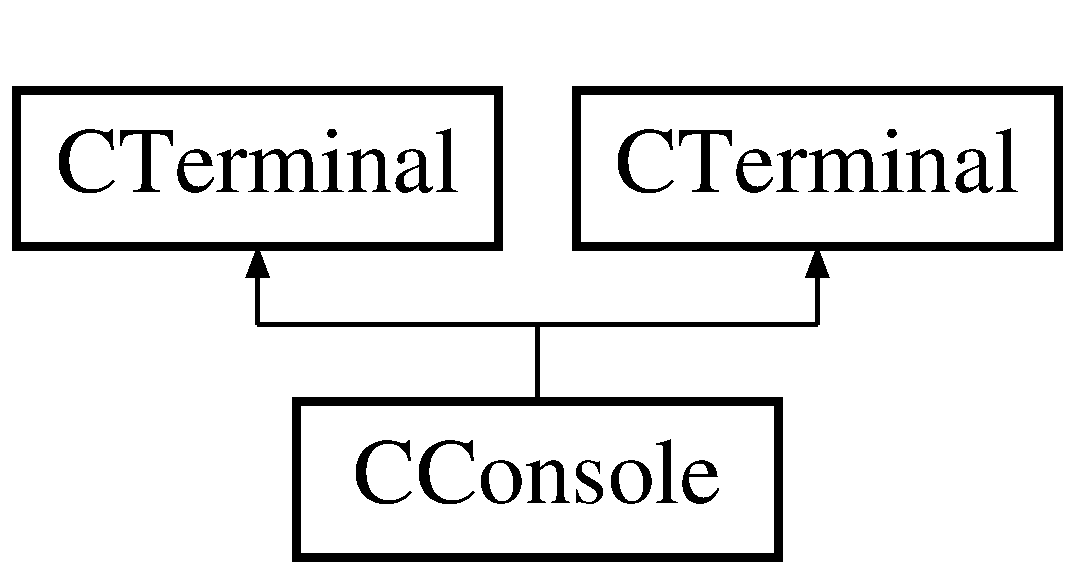
\includegraphics[height=2.000000cm]{class_c_console}
\end{center}
\end{figure}
\subsection*{Public Member Functions}
\begin{DoxyCompactItemize}
\item 
\mbox{\hyperlink{class_c_console_a9ff3a14fd32fec13a98fd6064d26c861}{C\+Console}} ()
\begin{DoxyCompactList}\small\item\em \mbox{\hyperlink{class_c_console}{C\+Console}} constructor. This method create a \mbox{\hyperlink{class_c_console}{C\+Console}} object instance. \end{DoxyCompactList}\item 
\mbox{\Hypertarget{class_c_console_a43dc951b007232f5cc98230c160813f3}\label{class_c_console_a43dc951b007232f5cc98230c160813f3}} 
\mbox{\hyperlink{class_c_console_a43dc951b007232f5cc98230c160813f3}{C\+Console}} (C\+Time $\ast$sys\+Ck)
\begin{DoxyCompactList}\small\item\em Class constructor. \end{DoxyCompactList}\item 
\mbox{\Hypertarget{class_c_console_a1d1ecc48fc4de70bfe0f6530c9d3bfc5}\label{class_c_console_a1d1ecc48fc4de70bfe0f6530c9d3bfc5}} 
\mbox{\hyperlink{class_c_console_a1d1ecc48fc4de70bfe0f6530c9d3bfc5}{$\sim$\+C\+Console}} ()
\begin{DoxyCompactList}\small\item\em Class destructor. \end{DoxyCompactList}\item 
void \mbox{\hyperlink{class_c_console_a23af1eebefd7cce94b4bdd5cc430e360}{write\+Log\+String}} (string str, bool new\+Line)
\begin{DoxyCompactList}\small\item\em Method to send strings for log information via console. \end{DoxyCompactList}\item 
void \mbox{\hyperlink{class_c_console_ad6f84380de57942510c8abfc5226f6c5}{write\+Log\+Integer}} (int num, bool new\+Line)
\begin{DoxyCompactList}\small\item\em Method to send integers for log information via console. \end{DoxyCompactList}\item 
bool \mbox{\hyperlink{class_c_console_a93d2d9f396de1137b6aefe87643ff7fe}{Read\+Command}} (char $\ast$com)
\end{DoxyCompactItemize}


\subsection{Detailed Description}
PC\textquotesingle{}s \mbox{\hyperlink{class_c_console}{C\+Console}} class implementation. 

UC\textquotesingle{}s \mbox{\hyperlink{class_c_console}{C\+Console}} class implementation.

This class implements the methods to initialize and access a command line interface. 

Definition at line 34 of file C\+O\+N\+S\+O\+L\+E\+\_\+\+P\+C.\+h.



\subsection{Constructor \& Destructor Documentation}
\mbox{\Hypertarget{class_c_console_a9ff3a14fd32fec13a98fd6064d26c861}\label{class_c_console_a9ff3a14fd32fec13a98fd6064d26c861}} 
\index{C\+Console@{C\+Console}!C\+Console@{C\+Console}}
\index{C\+Console@{C\+Console}!C\+Console@{C\+Console}}
\subsubsection{\texorpdfstring{C\+Console()}{CConsole()}}
{\footnotesize\ttfamily C\+Console\+::\+C\+Console (\begin{DoxyParamCaption}{ }\end{DoxyParamCaption})}



\mbox{\hyperlink{class_c_console}{C\+Console}} constructor. This method create a \mbox{\hyperlink{class_c_console}{C\+Console}} object instance. 

Class constructor. 

Definition at line 33 of file C\+O\+N\+S\+O\+L\+E\+\_\+\+P\+C.\+cpp.



\subsection{Member Function Documentation}
\mbox{\Hypertarget{class_c_console_a93d2d9f396de1137b6aefe87643ff7fe}\label{class_c_console_a93d2d9f396de1137b6aefe87643ff7fe}} 
\index{C\+Console@{C\+Console}!Read\+Command@{Read\+Command}}
\index{Read\+Command@{Read\+Command}!C\+Console@{C\+Console}}
\subsubsection{\texorpdfstring{Read\+Command()}{ReadCommand()}}
{\footnotesize\ttfamily bool C\+Console\+::\+Read\+Command (\begin{DoxyParamCaption}\item[{char $\ast$}]{com }\end{DoxyParamCaption})\hspace{0.3cm}{\ttfamily [virtual]}}

method verifies if there was some valid input from keyboard. If yes, put the input in com. 
\begin{DoxyParams}{Parameters}
{\em com} & -\/ pointer to char \\
\hline
\end{DoxyParams}
\begin{DoxyReturn}{Returns}
Return true if a valid input was received, false if no. 
\end{DoxyReturn}


Implements \mbox{\hyperlink{class_c_terminal}{C\+Terminal}}.



Definition at line 142 of file C\+O\+N\+S\+O\+L\+E\+\_\+\+P\+C.\+cpp.



Referenced by C\+Control\+::receive\+Command().

\mbox{\Hypertarget{class_c_console_ad6f84380de57942510c8abfc5226f6c5}\label{class_c_console_ad6f84380de57942510c8abfc5226f6c5}} 
\index{C\+Console@{C\+Console}!write\+Log\+Integer@{write\+Log\+Integer}}
\index{write\+Log\+Integer@{write\+Log\+Integer}!C\+Console@{C\+Console}}
\subsubsection{\texorpdfstring{write\+Log\+Integer()}{writeLogInteger()}}
{\footnotesize\ttfamily void C\+Console\+::write\+Log\+Integer (\begin{DoxyParamCaption}\item[{int}]{num,  }\item[{bool}]{new\+Line }\end{DoxyParamCaption})\hspace{0.3cm}{\ttfamily [virtual]}}



Method to send integers for log information via console. 


\begin{DoxyParams}{Parameters}
{\em num} & -\/ number to be sent, new\+Line -\/ if true, send a new\+Line (~\newline
) in the end of string. If false, doesn\textquotesingle{}t. \\
\hline
\end{DoxyParams}
\begin{DoxyReturn}{Returns}
none 
\end{DoxyReturn}


Implements \mbox{\hyperlink{class_c_terminal}{C\+Terminal}}.



Definition at line 117 of file C\+O\+N\+S\+O\+L\+E\+\_\+\+P\+C.\+cpp.

\mbox{\Hypertarget{class_c_console_a23af1eebefd7cce94b4bdd5cc430e360}\label{class_c_console_a23af1eebefd7cce94b4bdd5cc430e360}} 
\index{C\+Console@{C\+Console}!write\+Log\+String@{write\+Log\+String}}
\index{write\+Log\+String@{write\+Log\+String}!C\+Console@{C\+Console}}
\subsubsection{\texorpdfstring{write\+Log\+String()}{writeLogString()}}
{\footnotesize\ttfamily void C\+Console\+::write\+Log\+String (\begin{DoxyParamCaption}\item[{string}]{str,  }\item[{bool}]{new\+Line }\end{DoxyParamCaption})\hspace{0.3cm}{\ttfamily [virtual]}}



Method to send strings for log information via console. 


\begin{DoxyParams}{Parameters}
{\em str} & -\/ string to be sent, new\+Line -\/ if true, send a new\+Line (~\newline
) in the end of string. If false, doesn\textquotesingle{}t. \\
\hline
\end{DoxyParams}
\begin{DoxyReturn}{Returns}
none 
\end{DoxyReturn}


Implements \mbox{\hyperlink{class_c_terminal}{C\+Terminal}}.



Definition at line 92 of file C\+O\+N\+S\+O\+L\+E\+\_\+\+P\+C.\+cpp.



Referenced by C\+Control\+::commands\+Parser().



The documentation for this class was generated from the following files\+:\begin{DoxyCompactItemize}
\item 
C\+:/\+Users/\+User/\+Dropbox/\+U\+F\+S\+C/2018.\+2/\+O\+O/\+Projeto\+\_\+\+Final/fw/src/\mbox{\hyperlink{_c_o_n_s_o_l_e___p_c_8h}{C\+O\+N\+S\+O\+L\+E\+\_\+\+P\+C.\+h}}\item 
C\+:/\+Users/\+User/\+Dropbox/\+U\+F\+S\+C/2018.\+2/\+O\+O/\+Projeto\+\_\+\+Final/fw/src/\mbox{\hyperlink{_u_a_r_t___u_c_8h}{U\+A\+R\+T\+\_\+\+U\+C.\+h}}\item 
C\+:/\+Users/\+User/\+Dropbox/\+U\+F\+S\+C/2018.\+2/\+O\+O/\+Projeto\+\_\+\+Final/fw/src/\mbox{\hyperlink{_c_o_n_s_o_l_e___p_c_8cpp}{C\+O\+N\+S\+O\+L\+E\+\_\+\+P\+C.\+cpp}}\item 
C\+:/\+Users/\+User/\+Dropbox/\+U\+F\+S\+C/2018.\+2/\+O\+O/\+Projeto\+\_\+\+Final/fw/src/\mbox{\hyperlink{_u_a_r_t___u_c_8cpp}{U\+A\+R\+T\+\_\+\+U\+C.\+cpp}}\end{DoxyCompactItemize}

\hypertarget{class_c_control}{}\section{C\+Control Class Reference}
\label{class_c_control}\index{C\+Control@{C\+Control}}


\mbox{\hyperlink{class_c_control}{C\+Control}} class implementation.  




{\ttfamily \#include $<$C\+O\+N\+T\+R\+O\+L.\+h$>$}

\subsection*{Public Member Functions}
\begin{DoxyCompactItemize}
\item 
\mbox{\Hypertarget{class_c_control_a6498500ff403327b5770a3acebed1d93}\label{class_c_control_a6498500ff403327b5770a3acebed1d93}} 
\mbox{\hyperlink{class_c_control_a6498500ff403327b5770a3acebed1d93}{C\+Control}} ()
\begin{DoxyCompactList}\small\item\em G\+P\+IO constructor. This method create a C\+C\+O\+N\+T\+R\+OL object instance. \end{DoxyCompactList}\item 
\mbox{\Hypertarget{class_c_control_ab2ae420ef75b010c0c9078e597781105}\label{class_c_control_ab2ae420ef75b010c0c9078e597781105}} 
\mbox{\hyperlink{class_c_control_ab2ae420ef75b010c0c9078e597781105}{$\sim$\+C\+Control}} ()
\begin{DoxyCompactList}\small\item\em Class destructor. \end{DoxyCompactList}\item 
void \mbox{\hyperlink{class_c_control_aa997117cf869f0e31dbb1f87f29ae8bf}{message\+Manager}} (void)
\begin{DoxyCompactList}\small\item\em This method coordinate timming and priorites of the messages to be shown at the display considering the priorities as F\+SM actions $>$ Date/\+Time information $>$ advertising. \end{DoxyCompactList}\item 
void \mbox{\hyperlink{class_c_control_ab698c7d1945864d1f5c35e091de1ab22}{receive\+Command}} (void)
\begin{DoxyCompactList}\small\item\em Method to receive a command from console and put it in the queue to be parsed. \end{DoxyCompactList}\item 
void \mbox{\hyperlink{class_c_control_a0ebf3ab01f3ea77f261b630ed2541f9d}{commands\+Parser}} (void)
\begin{DoxyCompactList}\small\item\em Method parser the commands received from the commands queue. \end{DoxyCompactList}\end{DoxyCompactItemize}


\subsection{Detailed Description}
\mbox{\hyperlink{class_c_control}{C\+Control}} class implementation. 

This class implements the methods to manager the messages and the commands of the system. 

Definition at line 50 of file C\+O\+N\+T\+R\+O\+L.\+h.



\subsection{Member Function Documentation}
\mbox{\Hypertarget{class_c_control_a0ebf3ab01f3ea77f261b630ed2541f9d}\label{class_c_control_a0ebf3ab01f3ea77f261b630ed2541f9d}} 
\index{C\+Control@{C\+Control}!commands\+Parser@{commands\+Parser}}
\index{commands\+Parser@{commands\+Parser}!C\+Control@{C\+Control}}
\subsubsection{\texorpdfstring{commands\+Parser()}{commandsParser()}}
{\footnotesize\ttfamily void C\+Control\+::commands\+Parser (\begin{DoxyParamCaption}\item[{void}]{ }\end{DoxyParamCaption})}



Method parser the commands received from the commands queue. 


\begin{DoxyParams}{Parameters}
{\em none} & \\
\hline
\end{DoxyParams}
\begin{DoxyReturn}{Returns}
none 
\end{DoxyReturn}


Definition at line 142 of file C\+O\+N\+T\+R\+O\+L.\+cpp.



References Cqueue$<$ T $>$\+::get\+Size(), Cqueue$<$ T $>$\+::pop\+Front(), Cqueue$<$ T $>$\+::push\+Back(), and C\+Console\+::write\+Log\+String().

\mbox{\Hypertarget{class_c_control_aa997117cf869f0e31dbb1f87f29ae8bf}\label{class_c_control_aa997117cf869f0e31dbb1f87f29ae8bf}} 
\index{C\+Control@{C\+Control}!message\+Manager@{message\+Manager}}
\index{message\+Manager@{message\+Manager}!C\+Control@{C\+Control}}
\subsubsection{\texorpdfstring{message\+Manager()}{messageManager()}}
{\footnotesize\ttfamily void C\+Control\+::message\+Manager (\begin{DoxyParamCaption}\item[{void}]{ }\end{DoxyParamCaption})}



This method coordinate timming and priorites of the messages to be shown at the display considering the priorities as F\+SM actions $>$ Date/\+Time information $>$ advertising. 


\begin{DoxyParams}{Parameters}
{\em none} & \\
\hline
\end{DoxyParams}
\begin{DoxyReturn}{Returns}
none 
\end{DoxyReturn}


Definition at line 54 of file C\+O\+N\+T\+R\+O\+L.\+cpp.



References Cqueue$<$ T $>$\+::check\+Empty().

\mbox{\Hypertarget{class_c_control_ab698c7d1945864d1f5c35e091de1ab22}\label{class_c_control_ab698c7d1945864d1f5c35e091de1ab22}} 
\index{C\+Control@{C\+Control}!receive\+Command@{receive\+Command}}
\index{receive\+Command@{receive\+Command}!C\+Control@{C\+Control}}
\subsubsection{\texorpdfstring{receive\+Command()}{receiveCommand()}}
{\footnotesize\ttfamily void C\+Control\+::receive\+Command (\begin{DoxyParamCaption}\item[{void}]{ }\end{DoxyParamCaption})}



Method to receive a command from console and put it in the queue to be parsed. 


\begin{DoxyParams}{Parameters}
{\em none} & \\
\hline
\end{DoxyParams}
\begin{DoxyReturn}{Returns}
none 
\end{DoxyReturn}


Definition at line 127 of file C\+O\+N\+T\+R\+O\+L.\+cpp.



References Cqueue$<$ T $>$\+::push\+Back(), and C\+Console\+::\+Read\+Command().



The documentation for this class was generated from the following files\+:\begin{DoxyCompactItemize}
\item 
C\+:/\+Users/\+User/\+Dropbox/\+U\+F\+S\+C/2018.\+2/\+O\+O/\+Projeto\+\_\+\+Final/fw/src/\mbox{\hyperlink{_c_o_n_t_r_o_l_8h}{C\+O\+N\+T\+R\+O\+L.\+h}}\item 
C\+:/\+Users/\+User/\+Dropbox/\+U\+F\+S\+C/2018.\+2/\+O\+O/\+Projeto\+\_\+\+Final/fw/src/\mbox{\hyperlink{_c_o_n_t_r_o_l_8cpp}{C\+O\+N\+T\+R\+O\+L.\+cpp}}\end{DoxyCompactItemize}

\hypertarget{class_c_date_time}{}\section{C\+Date\+Time Class Reference}
\label{class_c_date_time}\index{C\+Date\+Time@{C\+Date\+Time}}


System\textquotesingle{}s \mbox{\hyperlink{class_c_date_time}{C\+Date\+Time}} class implementation.  




{\ttfamily \#include $<$D\+A\+T\+E\+\_\+\+T\+I\+M\+E.\+h$>$}



Inherited by C\+Time, and C\+Time.

\subsection*{Public Member Functions}
\begin{DoxyCompactItemize}
\item 
\mbox{\Hypertarget{class_c_date_time_a84f3f82e4856f510db8cace1e2c4b9a7}\label{class_c_date_time_a84f3f82e4856f510db8cace1e2c4b9a7}} 
\mbox{\hyperlink{class_c_date_time_a84f3f82e4856f510db8cace1e2c4b9a7}{C\+Date\+Time}} ()
\begin{DoxyCompactList}\small\item\em Class constructor. \end{DoxyCompactList}\item 
\mbox{\Hypertarget{class_c_date_time_aba2df38e58c26268a205d5e54a5d21bd}\label{class_c_date_time_aba2df38e58c26268a205d5e54a5d21bd}} 
\mbox{\hyperlink{class_c_date_time_aba2df38e58c26268a205d5e54a5d21bd}{C\+Date\+Time}} (long int sck)
\begin{DoxyCompactList}\small\item\em Class constructor. \end{DoxyCompactList}\item 
\mbox{\Hypertarget{class_c_date_time_a1412c07bae2ac253df8d4708e0037162}\label{class_c_date_time_a1412c07bae2ac253df8d4708e0037162}} 
\mbox{\hyperlink{class_c_date_time_a1412c07bae2ac253df8d4708e0037162}{$\sim$\+C\+Date\+Time}} ()
\begin{DoxyCompactList}\small\item\em Class destructor. \end{DoxyCompactList}\end{DoxyCompactItemize}


\subsection{Detailed Description}
System\textquotesingle{}s \mbox{\hyperlink{class_c_date_time}{C\+Date\+Time}} class implementation. 

This class implements the virtual methods to access the system time. 

Definition at line 33 of file D\+A\+T\+E\+\_\+\+T\+I\+M\+E.\+h.



The documentation for this class was generated from the following files\+:\begin{DoxyCompactItemize}
\item 
C\+:/\+Users/\+User/\+Dropbox/\+U\+F\+S\+C/2018.\+2/\+O\+O/\+Projeto\+\_\+\+Final/fw/src/\mbox{\hyperlink{_d_a_t_e___t_i_m_e_8h}{D\+A\+T\+E\+\_\+\+T\+I\+M\+E.\+h}}\item 
C\+:/\+Users/\+User/\+Dropbox/\+U\+F\+S\+C/2018.\+2/\+O\+O/\+Projeto\+\_\+\+Final/fw/src/\mbox{\hyperlink{_d_a_t_e___t_i_m_e_8cpp}{D\+A\+T\+E\+\_\+\+T\+I\+M\+E.\+cpp}}\end{DoxyCompactItemize}

\hypertarget{class_c_display}{}\section{C\+Display Class Reference}
\label{class_c_display}\index{C\+Display@{C\+Display}}


System\textquotesingle{}s Display class implementation.  




{\ttfamily \#include $<$D\+I\+S\+P\+L\+A\+Y.\+h$>$}

Inheritance diagram for C\+Display\+:\begin{figure}[H]
\begin{center}
\leavevmode
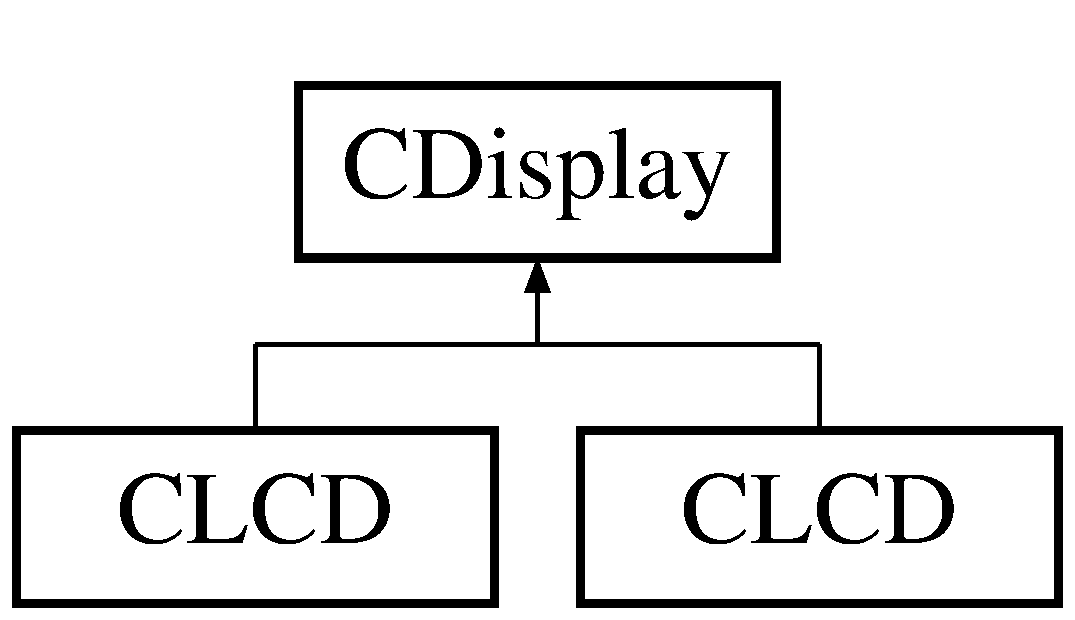
\includegraphics[height=2.000000cm]{class_c_display}
\end{center}
\end{figure}
\subsection*{Public Member Functions}
\begin{DoxyCompactItemize}
\item 
\mbox{\Hypertarget{class_c_display_aeab4454cf16b08e1b091c495be595269}\label{class_c_display_aeab4454cf16b08e1b091c495be595269}} 
\mbox{\hyperlink{class_c_display_aeab4454cf16b08e1b091c495be595269}{C\+Display}} ()
\begin{DoxyCompactList}\small\item\em Class constructor. \end{DoxyCompactList}\item 
\mbox{\Hypertarget{class_c_display_a15f66b785f2952394d199b9ca58e0f4b}\label{class_c_display_a15f66b785f2952394d199b9ca58e0f4b}} 
\mbox{\hyperlink{class_c_display_a15f66b785f2952394d199b9ca58e0f4b}{$\sim$\+C\+Display}} ()
\begin{DoxyCompactList}\small\item\em Class destructor. \end{DoxyCompactList}\end{DoxyCompactItemize}


\subsection{Detailed Description}
System\textquotesingle{}s Display class implementation. 

This class implements the virtual methods to access the display. 

Definition at line 33 of file D\+I\+S\+P\+L\+A\+Y.\+h.



The documentation for this class was generated from the following files\+:\begin{DoxyCompactItemize}
\item 
C\+:/\+Users/\+User/\+Dropbox/\+U\+F\+S\+C/2018.\+2/\+O\+O/\+Projeto\+\_\+\+Final/fw/src/\mbox{\hyperlink{_d_i_s_p_l_a_y_8h}{D\+I\+S\+P\+L\+A\+Y.\+h}}\item 
C\+:/\+Users/\+User/\+Dropbox/\+U\+F\+S\+C/2018.\+2/\+O\+O/\+Projeto\+\_\+\+Final/fw/src/D\+I\+S\+P\+L\+A\+Y.\+cpp\end{DoxyCompactItemize}

\hypertarget{class_c_f_s_m}{}\section{C\+F\+SM Class Reference}
\label{class_c_f_s_m}\index{C\+F\+SM@{C\+F\+SM}}


System\textquotesingle{}s \mbox{\hyperlink{class_c_f_s_m}{C\+F\+SM}} class implementation.  




{\ttfamily \#include $<$F\+S\+M.\+h$>$}

\subsection*{Public Member Functions}
\begin{DoxyCompactItemize}
\item 
\mbox{\Hypertarget{class_c_f_s_m_a84a43705322f53414f0f7fceeb9b26c6}\label{class_c_f_s_m_a84a43705322f53414f0f7fceeb9b26c6}} 
\mbox{\hyperlink{class_c_f_s_m_a84a43705322f53414f0f7fceeb9b26c6}{C\+F\+SM}} ()
\begin{DoxyCompactList}\small\item\em Class constructor. \end{DoxyCompactList}\item 
\mbox{\Hypertarget{class_c_f_s_m_a99c583f74a419101fe47dda8ad7423c7}\label{class_c_f_s_m_a99c583f74a419101fe47dda8ad7423c7}} 
\mbox{\hyperlink{class_c_f_s_m_a99c583f74a419101fe47dda8ad7423c7}{$\sim$\+C\+F\+SM}} ()
\begin{DoxyCompactList}\small\item\em Class destructor. \end{DoxyCompactList}\item 
void \mbox{\hyperlink{class_c_f_s_m_afce29c93915785baa519eb824efc938b}{change\+State}} (\mbox{\hyperlink{_f_s_m_8h_a7d59fd39d0fd81e92c4d689f0f6e1fab}{F\+S\+Mstate\+\_\+t}} new\+State)
\begin{DoxyCompactList}\small\item\em Method to change the state of the F\+SM. \end{DoxyCompactList}\item 
\mbox{\hyperlink{_f_s_m_8h_a7d59fd39d0fd81e92c4d689f0f6e1fab}{F\+S\+Mstate\+\_\+t}} \mbox{\hyperlink{class_c_f_s_m_a596ebe7fc03a0d1402fefc650f6c1777}{get\+State}} ()
\begin{DoxyCompactList}\small\item\em Method get the state of the F\+SM. \end{DoxyCompactList}\item 
void \mbox{\hyperlink{class_c_f_s_m_a5e7a63354d1088160e3d790bebb099af}{run\+F\+SM}} (\mbox{\hyperlink{class_cqueue}{Cqueue}}$<$ string $>$ $\ast$queueP)
\begin{DoxyCompactList}\small\item\em Method that implements the F\+SM. \end{DoxyCompactList}\end{DoxyCompactItemize}


\subsection{Detailed Description}
System\textquotesingle{}s \mbox{\hyperlink{class_c_f_s_m}{C\+F\+SM}} class implementation. 

This class implements the methods to run the F\+SM. 

Definition at line 43 of file F\+S\+M.\+h.



\subsection{Member Function Documentation}
\mbox{\Hypertarget{class_c_f_s_m_afce29c93915785baa519eb824efc938b}\label{class_c_f_s_m_afce29c93915785baa519eb824efc938b}} 
\index{C\+F\+SM@{C\+F\+SM}!change\+State@{change\+State}}
\index{change\+State@{change\+State}!C\+F\+SM@{C\+F\+SM}}
\subsubsection{\texorpdfstring{change\+State()}{changeState()}}
{\footnotesize\ttfamily void C\+F\+S\+M\+::change\+State (\begin{DoxyParamCaption}\item[{\mbox{\hyperlink{_f_s_m_8h_a7d59fd39d0fd81e92c4d689f0f6e1fab}{F\+S\+Mstate\+\_\+t}}}]{new\+State }\end{DoxyParamCaption})}



Method to change the state of the F\+SM. 


\begin{DoxyParams}{Parameters}
{\em new\+State} & -\/ new F\+SM state. \\
\hline
\end{DoxyParams}
\begin{DoxyReturn}{Returns}
none 
\end{DoxyReturn}


Definition at line 46 of file F\+S\+M.\+cpp.

\mbox{\Hypertarget{class_c_f_s_m_a596ebe7fc03a0d1402fefc650f6c1777}\label{class_c_f_s_m_a596ebe7fc03a0d1402fefc650f6c1777}} 
\index{C\+F\+SM@{C\+F\+SM}!get\+State@{get\+State}}
\index{get\+State@{get\+State}!C\+F\+SM@{C\+F\+SM}}
\subsubsection{\texorpdfstring{get\+State()}{getState()}}
{\footnotesize\ttfamily \mbox{\hyperlink{_f_s_m_8h_a7d59fd39d0fd81e92c4d689f0f6e1fab}{F\+S\+Mstate\+\_\+t}} C\+F\+S\+M\+::get\+State (\begin{DoxyParamCaption}{ }\end{DoxyParamCaption})}



Method get the state of the F\+SM. 


\begin{DoxyParams}{Parameters}
{\em none} & \\
\hline
\end{DoxyParams}
\begin{DoxyReturn}{Returns}
actual F\+SM state 
\end{DoxyReturn}


Definition at line 56 of file F\+S\+M.\+cpp.

\mbox{\Hypertarget{class_c_f_s_m_a5e7a63354d1088160e3d790bebb099af}\label{class_c_f_s_m_a5e7a63354d1088160e3d790bebb099af}} 
\index{C\+F\+SM@{C\+F\+SM}!run\+F\+SM@{run\+F\+SM}}
\index{run\+F\+SM@{run\+F\+SM}!C\+F\+SM@{C\+F\+SM}}
\subsubsection{\texorpdfstring{run\+F\+S\+M()}{runFSM()}}
{\footnotesize\ttfamily void C\+F\+S\+M\+::run\+F\+SM (\begin{DoxyParamCaption}\item[{\mbox{\hyperlink{class_cqueue}{Cqueue}}$<$ string $>$ $\ast$}]{queueP }\end{DoxyParamCaption})}



Method that implements the F\+SM. 


\begin{DoxyParams}{Parameters}
{\em queueP} & -\/ pointer to a queue used to send messages informing the actions executed by the F\+SM. \\
\hline
\end{DoxyParams}
\begin{DoxyReturn}{Returns}
none 
\end{DoxyReturn}


Definition at line 67 of file F\+S\+M.\+cpp.



The documentation for this class was generated from the following files\+:\begin{DoxyCompactItemize}
\item 
C\+:/\+Users/\+User/\+Dropbox/\+U\+F\+S\+C/2018.\+2/\+O\+O/\+Projeto\+\_\+\+Final/fw/src/\mbox{\hyperlink{_f_s_m_8h}{F\+S\+M.\+h}}\item 
C\+:/\+Users/\+User/\+Dropbox/\+U\+F\+S\+C/2018.\+2/\+O\+O/\+Projeto\+\_\+\+Final/fw/src/F\+S\+M.\+cpp\end{DoxyCompactItemize}

\hypertarget{class_c_g_p_i_o}{}\section{C\+G\+P\+IO Class Reference}
\label{class_c_g_p_i_o}\index{C\+G\+P\+IO@{C\+G\+P\+IO}}


PC\textquotesingle{}s \mbox{\hyperlink{class_c_g_p_i_o}{C\+G\+P\+IO}} class implementation.  




{\ttfamily \#include $<$G\+P\+I\+O\+\_\+\+P\+C.\+h$>$}

Inheritance diagram for C\+G\+P\+IO\+:\begin{figure}[H]
\begin{center}
\leavevmode
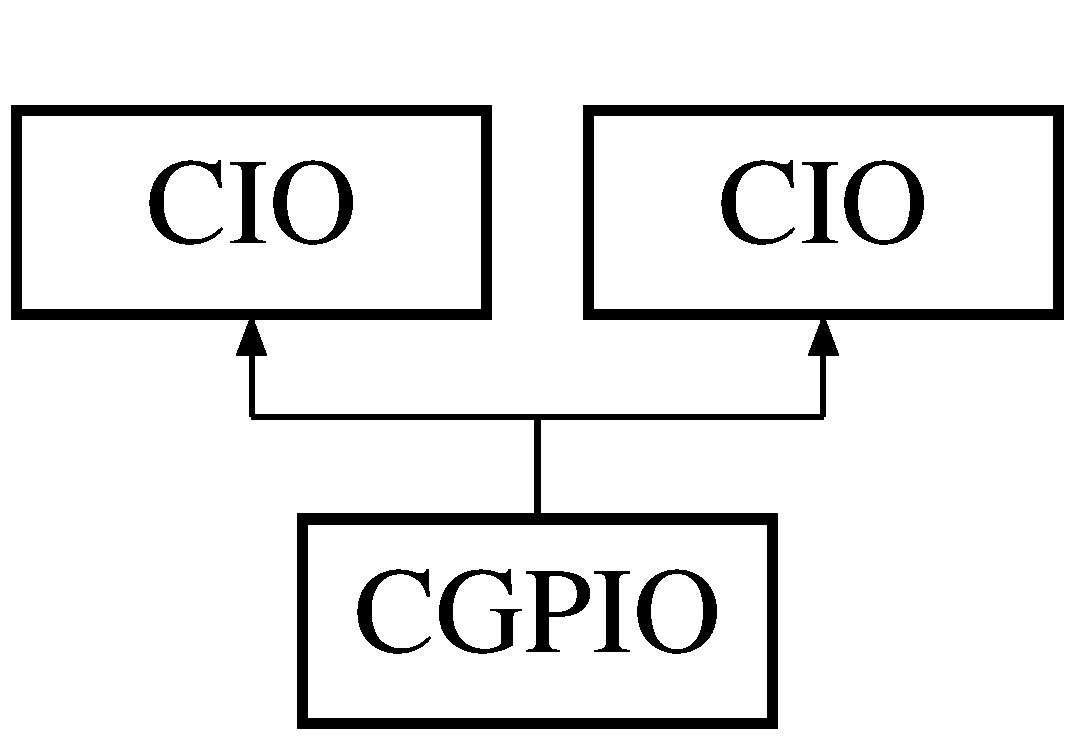
\includegraphics[height=2.000000cm]{class_c_g_p_i_o}
\end{center}
\end{figure}
\subsection*{Public Member Functions}
\begin{DoxyCompactItemize}
\item 
\mbox{\hyperlink{class_c_g_p_i_o_a9d4e47555fcac0233f6f3ebe36153863}{C\+G\+P\+IO}} ()
\begin{DoxyCompactList}\small\item\em Class constructor. \end{DoxyCompactList}\item 
\mbox{\Hypertarget{class_c_g_p_i_o_a0751442fbab665ca1525a51361e4cfa5}\label{class_c_g_p_i_o_a0751442fbab665ca1525a51361e4cfa5}} 
\mbox{\hyperlink{class_c_g_p_i_o_a0751442fbab665ca1525a51361e4cfa5}{$\sim$\+C\+G\+P\+IO}} ()
\begin{DoxyCompactList}\small\item\em Class destructor. \end{DoxyCompactList}\item 
void \mbox{\hyperlink{class_c_g_p_i_o_a6168af74d745d959e90deddb5c298385}{read\+Inputs}} (\mbox{\hyperlink{class_cqueue}{Cqueue}}$<$ string $>$ $\ast$queueP)
\begin{DoxyCompactList}\small\item\em This method manage the G\+P\+I\+Os input. \end{DoxyCompactList}\item 
void \mbox{\hyperlink{class_c_g_p_i_o_a512879113a7515680c76fac8852f69cc}{write\+Outputs}} (\mbox{\hyperlink{class_cqueue}{Cqueue}}$<$ string $>$ $\ast$queueP)
\begin{DoxyCompactList}\small\item\em Method responsible to update the outputs. \end{DoxyCompactList}\end{DoxyCompactItemize}
\subsection*{Static Protected Member Functions}
\begin{DoxyCompactItemize}
\item 
static \mbox{\hyperlink{class_c_g_p_i_o}{C\+G\+P\+IO}} $\ast$ \mbox{\hyperlink{class_c_g_p_i_o_a5fda50ad2bf1efc087793542ee3c88af}{get\+Current}} (void)
\begin{DoxyCompactList}\small\item\em Method to obtain the value of the current pointer. \end{DoxyCompactList}\item 
static void \mbox{\hyperlink{class_c_g_p_i_o_a06bc11242ea8f85b5d71419bf70ef674}{set\+Current}} (\mbox{\hyperlink{class_c_g_p_i_o}{C\+G\+P\+IO}} $\ast$gpio)
\begin{DoxyCompactList}\small\item\em Method to set the value of the current pointer. \end{DoxyCompactList}\end{DoxyCompactItemize}
\subsection*{Static Protected Attributes}
\begin{DoxyCompactItemize}
\item 
static \mbox{\hyperlink{class_c_g_p_i_o}{C\+G\+P\+IO}} $\ast$ \mbox{\hyperlink{class_c_g_p_i_o_a21d3b21fbb921eca646b24582fb5c43f}{current}} = nullptr
\end{DoxyCompactItemize}
\subsection*{Friends}
\begin{DoxyCompactItemize}
\item 
void \mbox{\hyperlink{class_c_g_p_i_o_a94ed9692de8f805af0517790cb06b71c}{G\+P\+I\+O\+I\+SR}} ()
\begin{DoxyCompactList}\small\item\em friend function that performs the I\+SR treatment to read the inputs. \end{DoxyCompactList}\end{DoxyCompactItemize}


\subsection{Detailed Description}
PC\textquotesingle{}s \mbox{\hyperlink{class_c_g_p_i_o}{C\+G\+P\+IO}} class implementation. 

uC\textquotesingle{}s \mbox{\hyperlink{class_c_g_p_i_o}{C\+G\+P\+IO}} class implementation.

This class implements the methods to initialize and access the PC\textquotesingle{}s G\+P\+IO.

This class implements the methods to initialize and access the microcontroller\textquotesingle{}s G\+P\+IO. 

Definition at line 32 of file G\+P\+I\+O\+\_\+\+P\+C.\+h.



\subsection{Constructor \& Destructor Documentation}
\mbox{\Hypertarget{class_c_g_p_i_o_a9d4e47555fcac0233f6f3ebe36153863}\label{class_c_g_p_i_o_a9d4e47555fcac0233f6f3ebe36153863}} 
\index{C\+G\+P\+IO@{C\+G\+P\+IO}!C\+G\+P\+IO@{C\+G\+P\+IO}}
\index{C\+G\+P\+IO@{C\+G\+P\+IO}!C\+G\+P\+IO@{C\+G\+P\+IO}}
\subsubsection{\texorpdfstring{C\+G\+P\+I\+O()}{CGPIO()}}
{\footnotesize\ttfamily C\+G\+P\+I\+O\+::\+C\+G\+P\+IO (\begin{DoxyParamCaption}{ }\end{DoxyParamCaption})}



Class constructor. 

G\+P\+IO constructor. This method create a G\+P\+IO object instance. Configuring G\+P\+IO interrupts 

Definition at line 31 of file G\+P\+I\+O\+\_\+\+P\+C.\+cpp.



\subsection{Member Function Documentation}
\mbox{\Hypertarget{class_c_g_p_i_o_a5fda50ad2bf1efc087793542ee3c88af}\label{class_c_g_p_i_o_a5fda50ad2bf1efc087793542ee3c88af}} 
\index{C\+G\+P\+IO@{C\+G\+P\+IO}!get\+Current@{get\+Current}}
\index{get\+Current@{get\+Current}!C\+G\+P\+IO@{C\+G\+P\+IO}}
\subsubsection{\texorpdfstring{get\+Current()}{getCurrent()}}
{\footnotesize\ttfamily \mbox{\hyperlink{class_c_g_p_i_o}{C\+G\+P\+IO}} $\ast$ C\+G\+P\+I\+O\+::get\+Current (\begin{DoxyParamCaption}\item[{void}]{ }\end{DoxyParamCaption})\hspace{0.3cm}{\ttfamily [static]}, {\ttfamily [protected]}}



Method to obtain the value of the current pointer. 


\begin{DoxyParams}{Parameters}
{\em none} & \\
\hline
\end{DoxyParams}
\begin{DoxyReturn}{Returns}
\mbox{\hyperlink{class_c_g_p_i_o}{C\+G\+P\+IO}} class pointer 
\end{DoxyReturn}


Definition at line 182 of file G\+P\+I\+O\+\_\+\+U\+C.\+cpp.



References current.

\mbox{\Hypertarget{class_c_g_p_i_o_a6168af74d745d959e90deddb5c298385}\label{class_c_g_p_i_o_a6168af74d745d959e90deddb5c298385}} 
\index{C\+G\+P\+IO@{C\+G\+P\+IO}!read\+Inputs@{read\+Inputs}}
\index{read\+Inputs@{read\+Inputs}!C\+G\+P\+IO@{C\+G\+P\+IO}}
\subsubsection{\texorpdfstring{read\+Inputs()}{readInputs()}}
{\footnotesize\ttfamily void C\+G\+P\+I\+O\+::read\+Inputs (\begin{DoxyParamCaption}\item[{\mbox{\hyperlink{class_cqueue}{Cqueue}}$<$ string $>$ $\ast$}]{queueP }\end{DoxyParamCaption})\hspace{0.3cm}{\ttfamily [virtual]}}



This method manage the G\+P\+I\+Os input. 

This method was supposed to manage the G\+P\+I\+Os input, but in A\+RM platfor this fuction will be done by the I\+SR.


\begin{DoxyParams}{Parameters}
{\em queueP} & -\/ Pointer to an \mbox{\hyperlink{class_cqueue}{Cqueue}} object. \\
\hline
\end{DoxyParams}
\begin{DoxyReturn}{Returns}
none 
\end{DoxyReturn}


Implements \mbox{\hyperlink{class_c_i_o}{C\+IO}}.



Definition at line 49 of file G\+P\+I\+O\+\_\+\+P\+C.\+cpp.

\mbox{\Hypertarget{class_c_g_p_i_o_a06bc11242ea8f85b5d71419bf70ef674}\label{class_c_g_p_i_o_a06bc11242ea8f85b5d71419bf70ef674}} 
\index{C\+G\+P\+IO@{C\+G\+P\+IO}!set\+Current@{set\+Current}}
\index{set\+Current@{set\+Current}!C\+G\+P\+IO@{C\+G\+P\+IO}}
\subsubsection{\texorpdfstring{set\+Current()}{setCurrent()}}
{\footnotesize\ttfamily void C\+G\+P\+I\+O\+::set\+Current (\begin{DoxyParamCaption}\item[{\mbox{\hyperlink{class_c_g_p_i_o}{C\+G\+P\+IO}} $\ast$}]{gpio }\end{DoxyParamCaption})\hspace{0.3cm}{\ttfamily [static]}, {\ttfamily [protected]}}



Method to set the value of the current pointer. 


\begin{DoxyParams}{Parameters}
{\em gpio} & class pointer \\
\hline
\end{DoxyParams}
\begin{DoxyReturn}{Returns}
none 
\end{DoxyReturn}


Definition at line 192 of file G\+P\+I\+O\+\_\+\+U\+C.\+cpp.



References current.

\mbox{\Hypertarget{class_c_g_p_i_o_a512879113a7515680c76fac8852f69cc}\label{class_c_g_p_i_o_a512879113a7515680c76fac8852f69cc}} 
\index{C\+G\+P\+IO@{C\+G\+P\+IO}!write\+Outputs@{write\+Outputs}}
\index{write\+Outputs@{write\+Outputs}!C\+G\+P\+IO@{C\+G\+P\+IO}}
\subsubsection{\texorpdfstring{write\+Outputs()}{writeOutputs()}}
{\footnotesize\ttfamily void C\+G\+P\+I\+O\+::write\+Outputs (\begin{DoxyParamCaption}\item[{\mbox{\hyperlink{class_cqueue}{Cqueue}}$<$ string $>$ $\ast$}]{queueP }\end{DoxyParamCaption})\hspace{0.3cm}{\ttfamily [virtual]}}



Method responsible to update the outputs. 


\begin{DoxyParams}{Parameters}
{\em queueP} & -\/ Pointer to an \mbox{\hyperlink{class_cqueue}{Cqueue}} object. \\
\hline
\end{DoxyParams}
\begin{DoxyReturn}{Returns}
none 
\end{DoxyReturn}


Implements \mbox{\hyperlink{class_c_i_o}{C\+IO}}.



Definition at line 120 of file G\+P\+I\+O\+\_\+\+P\+C.\+cpp.



\subsection{Friends And Related Function Documentation}
\mbox{\Hypertarget{class_c_g_p_i_o_a94ed9692de8f805af0517790cb06b71c}\label{class_c_g_p_i_o_a94ed9692de8f805af0517790cb06b71c}} 
\index{C\+G\+P\+IO@{C\+G\+P\+IO}!G\+P\+I\+O\+I\+SR@{G\+P\+I\+O\+I\+SR}}
\index{G\+P\+I\+O\+I\+SR@{G\+P\+I\+O\+I\+SR}!C\+G\+P\+IO@{C\+G\+P\+IO}}
\subsubsection{\texorpdfstring{G\+P\+I\+O\+I\+SR}{GPIOISR}}
{\footnotesize\ttfamily void G\+P\+I\+O\+I\+SR (\begin{DoxyParamCaption}\item[{void}]{ }\end{DoxyParamCaption})\hspace{0.3cm}{\ttfamily [friend]}}



friend function that performs the I\+SR treatment to read the inputs. 


\begin{DoxyParams}{Parameters}
{\em none} & \\
\hline
\end{DoxyParams}
\begin{DoxyReturn}{Returns}
none 
\end{DoxyReturn}


Definition at line 202 of file G\+P\+I\+O\+\_\+\+U\+C.\+cpp.



\subsection{Member Data Documentation}
\mbox{\Hypertarget{class_c_g_p_i_o_a21d3b21fbb921eca646b24582fb5c43f}\label{class_c_g_p_i_o_a21d3b21fbb921eca646b24582fb5c43f}} 
\index{C\+G\+P\+IO@{C\+G\+P\+IO}!current@{current}}
\index{current@{current}!C\+G\+P\+IO@{C\+G\+P\+IO}}
\subsubsection{\texorpdfstring{current}{current}}
{\footnotesize\ttfamily \mbox{\hyperlink{class_c_g_p_i_o}{C\+G\+P\+IO}} $\ast$ C\+G\+P\+I\+O\+::current = nullptr\hspace{0.3cm}{\ttfamily [static]}, {\ttfamily [protected]}}

Pointer used to identy the object instatiated used for I\+SR purposes 

Definition at line 54 of file G\+P\+I\+O\+\_\+\+U\+C.\+h.



Referenced by get\+Current(), and set\+Current().



The documentation for this class was generated from the following files\+:\begin{DoxyCompactItemize}
\item 
C\+:/\+Users/\+User/\+Dropbox/\+U\+F\+S\+C/2018.\+2/\+O\+O/\+Projeto\+\_\+\+Final/fw/src/\mbox{\hyperlink{_g_p_i_o___p_c_8h}{G\+P\+I\+O\+\_\+\+P\+C.\+h}}\item 
C\+:/\+Users/\+User/\+Dropbox/\+U\+F\+S\+C/2018.\+2/\+O\+O/\+Projeto\+\_\+\+Final/fw/src/\mbox{\hyperlink{_g_p_i_o___u_c_8h}{G\+P\+I\+O\+\_\+\+U\+C.\+h}}\item 
C\+:/\+Users/\+User/\+Dropbox/\+U\+F\+S\+C/2018.\+2/\+O\+O/\+Projeto\+\_\+\+Final/fw/src/G\+P\+I\+O\+\_\+\+P\+C.\+cpp\item 
C\+:/\+Users/\+User/\+Dropbox/\+U\+F\+S\+C/2018.\+2/\+O\+O/\+Projeto\+\_\+\+Final/fw/src/\mbox{\hyperlink{_g_p_i_o___u_c_8cpp}{G\+P\+I\+O\+\_\+\+U\+C.\+cpp}}\end{DoxyCompactItemize}

\hypertarget{class_c_i_o}{}\section{C\+IO Class Reference}
\label{class_c_i_o}\index{C\+IO@{C\+IO}}


System\textquotesingle{}s IO class implementation.  




{\ttfamily \#include $<$I\+O.\+h$>$}

Inheritance diagram for C\+IO\+:\begin{figure}[H]
\begin{center}
\leavevmode
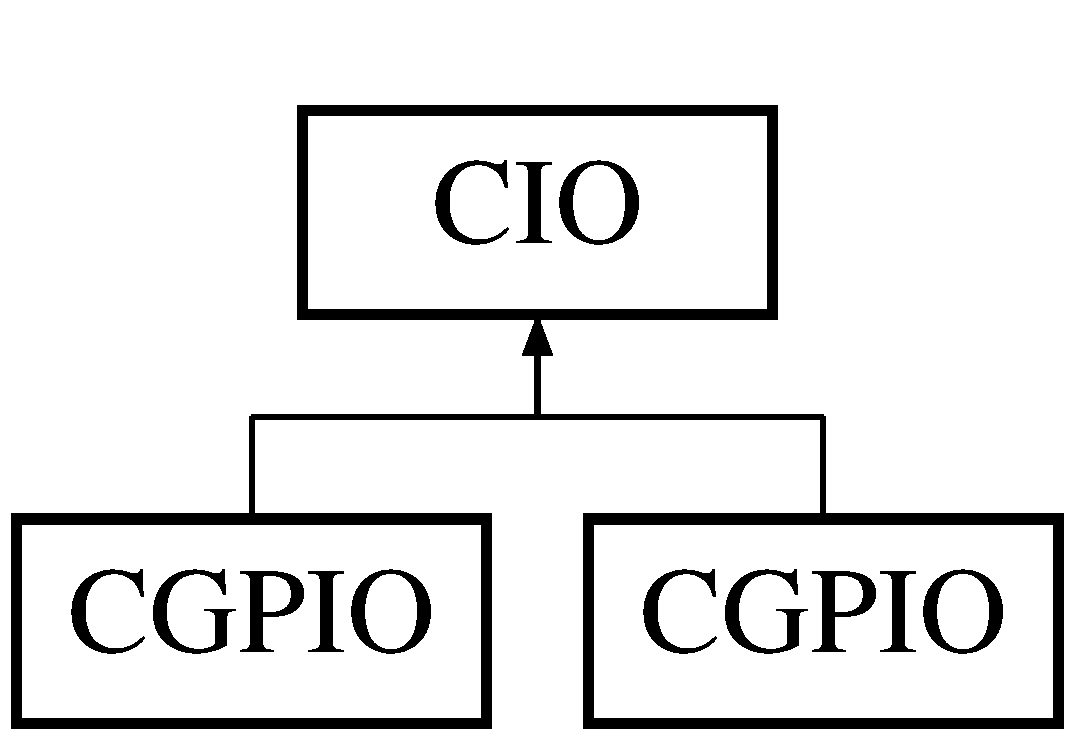
\includegraphics[height=2.000000cm]{class_c_i_o}
\end{center}
\end{figure}
\subsection*{Public Member Functions}
\begin{DoxyCompactItemize}
\item 
\mbox{\Hypertarget{class_c_i_o_a3359eaeb579531915933aa67d2fb02fd}\label{class_c_i_o_a3359eaeb579531915933aa67d2fb02fd}} 
\mbox{\hyperlink{class_c_i_o_a3359eaeb579531915933aa67d2fb02fd}{C\+IO}} ()
\begin{DoxyCompactList}\small\item\em Class constructor. \end{DoxyCompactList}\item 
\mbox{\Hypertarget{class_c_i_o_ae35aa920244299f614fbc9c7d1edc4de}\label{class_c_i_o_ae35aa920244299f614fbc9c7d1edc4de}} 
\mbox{\hyperlink{class_c_i_o_ae35aa920244299f614fbc9c7d1edc4de}{$\sim$\+C\+IO}} ()
\begin{DoxyCompactList}\small\item\em Class destructor. \end{DoxyCompactList}\item 
void \mbox{\hyperlink{class_c_i_o_ac61124eef35d5b751783010b39b24b0d}{set\+Input}} (int flag)
\begin{DoxyCompactList}\small\item\em Method to set an input flag. \end{DoxyCompactList}\item 
void \mbox{\hyperlink{class_c_i_o_a5fddf5dbe86f9baac7e2c75dcd9d35e6}{clear\+Input}} (int flag)
\begin{DoxyCompactList}\small\item\em Method to clear an input flag. \end{DoxyCompactList}\item 
bool \mbox{\hyperlink{class_c_i_o_aa87a99ef2b17c9243a745a6ec90fc5ef}{get\+Input}} (int flag)
\begin{DoxyCompactList}\small\item\em Method to get an input flag. \end{DoxyCompactList}\item 
void \mbox{\hyperlink{class_c_i_o_afc99e1a01c6de3f5f6126db69f8fd00e}{set\+Output}} (int flag)
\begin{DoxyCompactList}\small\item\em Method to set an output flag. \end{DoxyCompactList}\item 
void \mbox{\hyperlink{class_c_i_o_aa37612a9e9adfce7bf9b3a943bf961de}{clear\+Output}} (int flag)
\begin{DoxyCompactList}\small\item\em Method to clear an output flag. \end{DoxyCompactList}\item 
bool \mbox{\hyperlink{class_c_i_o_acc87c3bab69009087ff8cbc09dff88a3}{get\+Output}} (int flag)
\begin{DoxyCompactList}\small\item\em Method to get an output flag. \end{DoxyCompactList}\end{DoxyCompactItemize}


\subsection{Detailed Description}
System\textquotesingle{}s IO class implementation. 

This class implements the virtual methods to access the I\+Os. 

Definition at line 42 of file I\+O.\+h.



\subsection{Member Function Documentation}
\mbox{\Hypertarget{class_c_i_o_a5fddf5dbe86f9baac7e2c75dcd9d35e6}\label{class_c_i_o_a5fddf5dbe86f9baac7e2c75dcd9d35e6}} 
\index{C\+IO@{C\+IO}!clear\+Input@{clear\+Input}}
\index{clear\+Input@{clear\+Input}!C\+IO@{C\+IO}}
\subsubsection{\texorpdfstring{clear\+Input()}{clearInput()}}
{\footnotesize\ttfamily void C\+I\+O\+::clear\+Input (\begin{DoxyParamCaption}\item[{int}]{flag }\end{DoxyParamCaption})}



Method to clear an input flag. 


\begin{DoxyParams}{Parameters}
{\em flag} & -\/ Input to be cleared. \\
\hline
\end{DoxyParams}
\begin{DoxyReturn}{Returns}
none 
\end{DoxyReturn}


Definition at line 58 of file I\+O.\+cpp.

\mbox{\Hypertarget{class_c_i_o_aa37612a9e9adfce7bf9b3a943bf961de}\label{class_c_i_o_aa37612a9e9adfce7bf9b3a943bf961de}} 
\index{C\+IO@{C\+IO}!clear\+Output@{clear\+Output}}
\index{clear\+Output@{clear\+Output}!C\+IO@{C\+IO}}
\subsubsection{\texorpdfstring{clear\+Output()}{clearOutput()}}
{\footnotesize\ttfamily void C\+I\+O\+::clear\+Output (\begin{DoxyParamCaption}\item[{int}]{flag }\end{DoxyParamCaption})}



Method to clear an output flag. 


\begin{DoxyParams}{Parameters}
{\em flag} & -\/ Output to be clared. \\
\hline
\end{DoxyParams}
\begin{DoxyReturn}{Returns}
none 
\end{DoxyReturn}


Definition at line 88 of file I\+O.\+cpp.

\mbox{\Hypertarget{class_c_i_o_aa87a99ef2b17c9243a745a6ec90fc5ef}\label{class_c_i_o_aa87a99ef2b17c9243a745a6ec90fc5ef}} 
\index{C\+IO@{C\+IO}!get\+Input@{get\+Input}}
\index{get\+Input@{get\+Input}!C\+IO@{C\+IO}}
\subsubsection{\texorpdfstring{get\+Input()}{getInput()}}
{\footnotesize\ttfamily bool C\+I\+O\+::get\+Input (\begin{DoxyParamCaption}\item[{int}]{flag }\end{DoxyParamCaption})}



Method to get an input flag. 


\begin{DoxyParams}{Parameters}
{\em flag} & -\/ Input to be got. \\
\hline
\end{DoxyParams}
\begin{DoxyReturn}{Returns}
none 
\end{DoxyReturn}


Definition at line 68 of file I\+O.\+cpp.

\mbox{\Hypertarget{class_c_i_o_acc87c3bab69009087ff8cbc09dff88a3}\label{class_c_i_o_acc87c3bab69009087ff8cbc09dff88a3}} 
\index{C\+IO@{C\+IO}!get\+Output@{get\+Output}}
\index{get\+Output@{get\+Output}!C\+IO@{C\+IO}}
\subsubsection{\texorpdfstring{get\+Output()}{getOutput()}}
{\footnotesize\ttfamily bool C\+I\+O\+::get\+Output (\begin{DoxyParamCaption}\item[{int}]{flag }\end{DoxyParamCaption})}



Method to get an output flag. 


\begin{DoxyParams}{Parameters}
{\em flag} & -\/ Output to be got. \\
\hline
\end{DoxyParams}
\begin{DoxyReturn}{Returns}
none 
\end{DoxyReturn}


Definition at line 98 of file I\+O.\+cpp.

\mbox{\Hypertarget{class_c_i_o_ac61124eef35d5b751783010b39b24b0d}\label{class_c_i_o_ac61124eef35d5b751783010b39b24b0d}} 
\index{C\+IO@{C\+IO}!set\+Input@{set\+Input}}
\index{set\+Input@{set\+Input}!C\+IO@{C\+IO}}
\subsubsection{\texorpdfstring{set\+Input()}{setInput()}}
{\footnotesize\ttfamily void C\+I\+O\+::set\+Input (\begin{DoxyParamCaption}\item[{int}]{flag }\end{DoxyParamCaption})}



Method to set an input flag. 


\begin{DoxyParams}{Parameters}
{\em flag} & -\/ Input to be set. \\
\hline
\end{DoxyParams}
\begin{DoxyReturn}{Returns}
none 
\end{DoxyReturn}


Definition at line 48 of file I\+O.\+cpp.

\mbox{\Hypertarget{class_c_i_o_afc99e1a01c6de3f5f6126db69f8fd00e}\label{class_c_i_o_afc99e1a01c6de3f5f6126db69f8fd00e}} 
\index{C\+IO@{C\+IO}!set\+Output@{set\+Output}}
\index{set\+Output@{set\+Output}!C\+IO@{C\+IO}}
\subsubsection{\texorpdfstring{set\+Output()}{setOutput()}}
{\footnotesize\ttfamily void C\+I\+O\+::set\+Output (\begin{DoxyParamCaption}\item[{int}]{flag }\end{DoxyParamCaption})}



Method to set an output flag. 


\begin{DoxyParams}{Parameters}
{\em flag} & -\/ Output to be set. \\
\hline
\end{DoxyParams}
\begin{DoxyReturn}{Returns}
none 
\end{DoxyReturn}


Definition at line 78 of file I\+O.\+cpp.



The documentation for this class was generated from the following files\+:\begin{DoxyCompactItemize}
\item 
C\+:/\+Users/\+User/\+Dropbox/\+U\+F\+S\+C/2018.\+2/\+O\+O/\+Projeto\+\_\+\+Final/fw/src/\mbox{\hyperlink{_i_o_8h}{I\+O.\+h}}\item 
C\+:/\+Users/\+User/\+Dropbox/\+U\+F\+S\+C/2018.\+2/\+O\+O/\+Projeto\+\_\+\+Final/fw/src/\mbox{\hyperlink{_i_o_8cpp}{I\+O.\+cpp}}\end{DoxyCompactItemize}

\hypertarget{class_c_l_c_d}{}\section{C\+L\+CD Class Reference}
\label{class_c_l_c_d}\index{C\+L\+CD@{C\+L\+CD}}


\mbox{\hyperlink{class_c_l_c_d}{C\+L\+CD}} class implementation.  




{\ttfamily \#include $<$L\+C\+D\+\_\+\+U\+C.\+h$>$}

Inheritance diagram for C\+L\+CD\+:\begin{figure}[H]
\begin{center}
\leavevmode
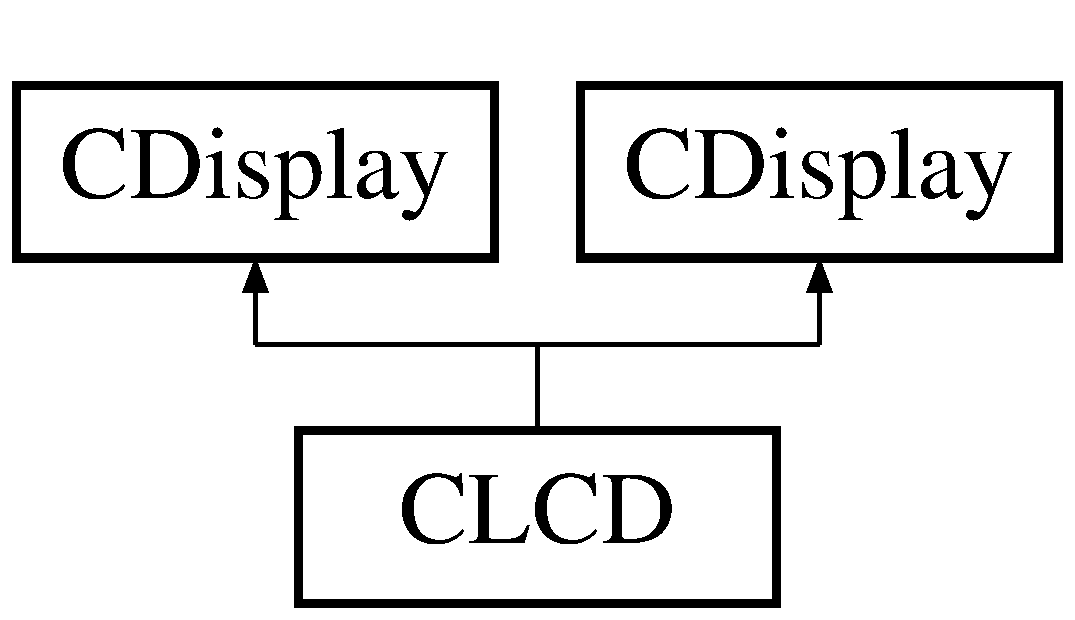
\includegraphics[height=2.000000cm]{class_c_l_c_d}
\end{center}
\end{figure}
\subsection*{Public Member Functions}
\begin{DoxyCompactItemize}
\item 
\mbox{\Hypertarget{class_c_l_c_d_ad695e45a239fa3190dc6192cff4c3a53}\label{class_c_l_c_d_ad695e45a239fa3190dc6192cff4c3a53}} 
\mbox{\hyperlink{class_c_l_c_d_ad695e45a239fa3190dc6192cff4c3a53}{C\+L\+CD}} ()
\begin{DoxyCompactList}\small\item\em Class constructor. \end{DoxyCompactList}\item 
\mbox{\Hypertarget{class_c_l_c_d_ac958cb7e31c6793cbbf2894b55671ddc}\label{class_c_l_c_d_ac958cb7e31c6793cbbf2894b55671ddc}} 
\mbox{\hyperlink{class_c_l_c_d_ac958cb7e31c6793cbbf2894b55671ddc}{$\sim$\+C\+L\+CD}} ()
\begin{DoxyCompactList}\small\item\em Class destructor. \end{DoxyCompactList}\item 
void \mbox{\hyperlink{class_c_l_c_d_aef53edad0951495613b38a0033a7d34c}{clear\+Screen}} ()
\begin{DoxyCompactList}\small\item\em Method to clear the entire L\+CD. \end{DoxyCompactList}\item 
void \mbox{\hyperlink{class_c_l_c_d_a48bc8230b2cef435c7972fd3e9522711}{write\+String}} (string str)
\begin{DoxyCompactList}\small\item\em Method to write a string in the L\+CD. \end{DoxyCompactList}\item 
void \mbox{\hyperlink{class_c_l_c_d_ab5547c17a38247c90db076b8c04baa17}{write\+Integer}} (int num)
\begin{DoxyCompactList}\small\item\em Method to write a number in the L\+CD. \end{DoxyCompactList}\item 
void \mbox{\hyperlink{class_c_l_c_d_af2d845b403b8978261a397cfe50f2fdc}{set\+Position}} (int x, int y)
\begin{DoxyCompactList}\small\item\em Method to the position to write in L\+CD. \end{DoxyCompactList}\end{DoxyCompactItemize}


\subsection{Detailed Description}
\mbox{\hyperlink{class_c_l_c_d}{C\+L\+CD}} class implementation. 

This class implements the methods to initialize and access the L\+CD from the microcontroller\textquotesingle{}s G\+P\+IO.

This class implements the methods to initialize and access the L\+CD from the PC\textquotesingle{}s. 

Definition at line 32 of file L\+C\+D\+\_\+\+U\+C.\+h.



\subsection{Member Function Documentation}
\mbox{\Hypertarget{class_c_l_c_d_aef53edad0951495613b38a0033a7d34c}\label{class_c_l_c_d_aef53edad0951495613b38a0033a7d34c}} 
\index{C\+L\+CD@{C\+L\+CD}!clear\+Screen@{clear\+Screen}}
\index{clear\+Screen@{clear\+Screen}!C\+L\+CD@{C\+L\+CD}}
\subsubsection{\texorpdfstring{clear\+Screen()}{clearScreen()}}
{\footnotesize\ttfamily void C\+L\+C\+D\+::clear\+Screen (\begin{DoxyParamCaption}{ }\end{DoxyParamCaption})\hspace{0.3cm}{\ttfamily [virtual]}}



Method to clear the entire L\+CD. 


\begin{DoxyParams}{Parameters}
{\em none} & \\
\hline
\end{DoxyParams}
\begin{DoxyReturn}{Returns}
none 
\end{DoxyReturn}


Implements \mbox{\hyperlink{class_c_display}{C\+Display}}.



Definition at line 81 of file L\+C\+D\+\_\+\+U\+C.\+cpp.



References L\+C\+D\+Clear().

\mbox{\Hypertarget{class_c_l_c_d_af2d845b403b8978261a397cfe50f2fdc}\label{class_c_l_c_d_af2d845b403b8978261a397cfe50f2fdc}} 
\index{C\+L\+CD@{C\+L\+CD}!set\+Position@{set\+Position}}
\index{set\+Position@{set\+Position}!C\+L\+CD@{C\+L\+CD}}
\subsubsection{\texorpdfstring{set\+Position()}{setPosition()}}
{\footnotesize\ttfamily void C\+L\+C\+D\+::set\+Position (\begin{DoxyParamCaption}\item[{int}]{x,  }\item[{int}]{y }\end{DoxyParamCaption})\hspace{0.3cm}{\ttfamily [virtual]}}



Method to the position to write in L\+CD. 


\begin{DoxyParams}{Parameters}
{\em x} & -\/ is the column \\
\hline
{\em y} & -\/ is the page \\
\hline
\end{DoxyParams}
\begin{DoxyReturn}{Returns}
none 
\end{DoxyReturn}


Implements \mbox{\hyperlink{class_c_display}{C\+Display}}.



Definition at line 116 of file L\+C\+D\+\_\+\+U\+C.\+cpp.



References L\+C\+D\+Set\+Column(), and L\+C\+D\+Set\+Page().

\mbox{\Hypertarget{class_c_l_c_d_ab5547c17a38247c90db076b8c04baa17}\label{class_c_l_c_d_ab5547c17a38247c90db076b8c04baa17}} 
\index{C\+L\+CD@{C\+L\+CD}!write\+Integer@{write\+Integer}}
\index{write\+Integer@{write\+Integer}!C\+L\+CD@{C\+L\+CD}}
\subsubsection{\texorpdfstring{write\+Integer()}{writeInteger()}}
{\footnotesize\ttfamily void C\+L\+C\+D\+::write\+Integer (\begin{DoxyParamCaption}\item[{int}]{num }\end{DoxyParamCaption})\hspace{0.3cm}{\ttfamily [virtual]}}



Method to write a number in the L\+CD. 


\begin{DoxyParams}{Parameters}
{\em num} & -\/ number to write \\
\hline
\end{DoxyParams}
\begin{DoxyReturn}{Returns}
none 
\end{DoxyReturn}


Implements \mbox{\hyperlink{class_c_display}{C\+Display}}.



Definition at line 105 of file L\+C\+D\+\_\+\+U\+C.\+cpp.

\mbox{\Hypertarget{class_c_l_c_d_a48bc8230b2cef435c7972fd3e9522711}\label{class_c_l_c_d_a48bc8230b2cef435c7972fd3e9522711}} 
\index{C\+L\+CD@{C\+L\+CD}!write\+String@{write\+String}}
\index{write\+String@{write\+String}!C\+L\+CD@{C\+L\+CD}}
\subsubsection{\texorpdfstring{write\+String()}{writeString()}}
{\footnotesize\ttfamily void C\+L\+C\+D\+::write\+String (\begin{DoxyParamCaption}\item[{string}]{str }\end{DoxyParamCaption})\hspace{0.3cm}{\ttfamily [virtual]}}



Method to write a string in the L\+CD. 


\begin{DoxyParams}{Parameters}
{\em str} & -\/ string to write \\
\hline
\end{DoxyParams}
\begin{DoxyReturn}{Returns}
none 
\end{DoxyReturn}


Implements \mbox{\hyperlink{class_c_display}{C\+Display}}.



Definition at line 92 of file L\+C\+D\+\_\+\+U\+C.\+cpp.



References L\+C\+D\+Write\+String(), and times8.



The documentation for this class was generated from the following files\+:\begin{DoxyCompactItemize}
\item 
C\+:/\+Users/\+User/\+Dropbox/\+U\+F\+S\+C/2018.\+2/\+O\+O/\+Projeto\+\_\+\+Final/fw/src/\mbox{\hyperlink{_l_c_d___u_c_8h}{L\+C\+D\+\_\+\+U\+C.\+h}}\item 
C\+:/\+Users/\+User/\+Dropbox/\+U\+F\+S\+C/2018.\+2/\+O\+O/\+Projeto\+\_\+\+Final/fw/src/\mbox{\hyperlink{_s_c_r_e_e_n___p_c_8h}{S\+C\+R\+E\+E\+N\+\_\+\+P\+C.\+h}}\item 
C\+:/\+Users/\+User/\+Dropbox/\+U\+F\+S\+C/2018.\+2/\+O\+O/\+Projeto\+\_\+\+Final/fw/src/L\+C\+D\+\_\+\+U\+C.\+cpp\item 
C\+:/\+Users/\+User/\+Dropbox/\+U\+F\+S\+C/2018.\+2/\+O\+O/\+Projeto\+\_\+\+Final/fw/src/\mbox{\hyperlink{_s_c_r_e_e_n___p_c_8cpp}{S\+C\+R\+E\+E\+N\+\_\+\+P\+C.\+cpp}}\end{DoxyCompactItemize}

\hypertarget{class_cqueue}{}\section{Cqueue$<$ T $>$ Class Template Reference}
\label{class_cqueue}\index{Cqueue$<$ T $>$@{Cqueue$<$ T $>$}}


Queue implementation with generic node.  




{\ttfamily \#include $<$queue.\+hpp$>$}

\subsection*{Public Member Functions}
\begin{DoxyCompactItemize}
\item 
\mbox{\Hypertarget{class_cqueue_a51d056d90c0162bbbdf554a2d4af785b}\label{class_cqueue_a51d056d90c0162bbbdf554a2d4af785b}} 
\mbox{\hyperlink{class_cqueue_a51d056d90c0162bbbdf554a2d4af785b}{Cqueue}} ()
\begin{DoxyCompactList}\small\item\em Class constructor. \end{DoxyCompactList}\item 
\mbox{\Hypertarget{class_cqueue_a2946de536ff33e0d84f721ce2d90056a}\label{class_cqueue_a2946de536ff33e0d84f721ce2d90056a}} 
\mbox{\hyperlink{class_cqueue_a2946de536ff33e0d84f721ce2d90056a}{$\sim$\+Cqueue}} ()
\begin{DoxyCompactList}\small\item\em Class destructor. \end{DoxyCompactList}\item 
bool \mbox{\hyperlink{class_cqueue_a7c20a21cd08b993af7222796322ccaec}{check\+Empty}} ()
\begin{DoxyCompactList}\small\item\em Method to check if the queue is empty. \end{DoxyCompactList}\item 
int \mbox{\hyperlink{class_cqueue_ad9baee6f6676b1eb0f0dfe450ba38eb1}{get\+Size}} ()
\begin{DoxyCompactList}\small\item\em Method to obtain the number of nodes that a queue contains. \end{DoxyCompactList}\item 
void \mbox{\hyperlink{class_cqueue_a901e6cfb613e56c487297633feb479b1}{push\+Back}} (T)
\begin{DoxyCompactList}\small\item\em Method to create a node to insert new data at the end of teh queue. \end{DoxyCompactList}\item 
T \mbox{\hyperlink{class_cqueue_a77d4728406bf0777254695f164132f3a}{pop\+Front}} ()
\begin{DoxyCompactList}\small\item\em Method to get the data from the queue and delete the node used to store it. \end{DoxyCompactList}\end{DoxyCompactItemize}


\subsection{Detailed Description}
\subsubsection*{template$<$class T$>$\newline
class Cqueue$<$ T $>$}

Queue implementation with generic node. 

This template class implements the methods to initialize and access queues with generic nodes. 

Definition at line 33 of file queue.\+hpp.



\subsection{Member Function Documentation}
\mbox{\Hypertarget{class_cqueue_a7c20a21cd08b993af7222796322ccaec}\label{class_cqueue_a7c20a21cd08b993af7222796322ccaec}} 
\index{Cqueue@{Cqueue}!check\+Empty@{check\+Empty}}
\index{check\+Empty@{check\+Empty}!Cqueue@{Cqueue}}
\subsubsection{\texorpdfstring{check\+Empty()}{checkEmpty()}}
{\footnotesize\ttfamily template$<$class T $>$ \\
bool \mbox{\hyperlink{class_cqueue}{Cqueue}}$<$ T $>$\+::check\+Empty (\begin{DoxyParamCaption}{ }\end{DoxyParamCaption})}



Method to check if the queue is empty. 


\begin{DoxyParams}{Parameters}
{\em none} & \\
\hline
\end{DoxyParams}
\begin{DoxyReturn}{Returns}
bool -\/ T\+R\+UE if the queue is empty, F\+A\+L\+SE if it isn\textquotesingle{}t. 
\end{DoxyReturn}


Definition at line 74 of file queue.\+hpp.



Referenced by C\+Control\+::message\+Manager().

\mbox{\Hypertarget{class_cqueue_ad9baee6f6676b1eb0f0dfe450ba38eb1}\label{class_cqueue_ad9baee6f6676b1eb0f0dfe450ba38eb1}} 
\index{Cqueue@{Cqueue}!get\+Size@{get\+Size}}
\index{get\+Size@{get\+Size}!Cqueue@{Cqueue}}
\subsubsection{\texorpdfstring{get\+Size()}{getSize()}}
{\footnotesize\ttfamily template$<$class T $>$ \\
int \mbox{\hyperlink{class_cqueue}{Cqueue}}$<$ T $>$\+::get\+Size (\begin{DoxyParamCaption}{ }\end{DoxyParamCaption})}



Method to obtain the number of nodes that a queue contains. 


\begin{DoxyParams}{Parameters}
{\em none} & \\
\hline
\end{DoxyParams}
\begin{DoxyReturn}{Returns}
int -\/ number of nodes. 
\end{DoxyReturn}


Definition at line 85 of file queue.\+hpp.



Referenced by C\+Control\+::commands\+Parser().

\mbox{\Hypertarget{class_cqueue_a77d4728406bf0777254695f164132f3a}\label{class_cqueue_a77d4728406bf0777254695f164132f3a}} 
\index{Cqueue@{Cqueue}!pop\+Front@{pop\+Front}}
\index{pop\+Front@{pop\+Front}!Cqueue@{Cqueue}}
\subsubsection{\texorpdfstring{pop\+Front()}{popFront()}}
{\footnotesize\ttfamily template$<$class T $>$ \\
T \mbox{\hyperlink{class_cqueue}{Cqueue}}$<$ T $>$\+::pop\+Front (\begin{DoxyParamCaption}{ }\end{DoxyParamCaption})}



Method to get the data from the queue and delete the node used to store it. 


\begin{DoxyParams}{Parameters}
{\em none} & \\
\hline
\end{DoxyParams}
\begin{DoxyReturn}{Returns}
T -\/ generic data type information. 
\end{DoxyReturn}


Definition at line 120 of file queue.\+hpp.



Referenced by C\+Control\+::commands\+Parser().

\mbox{\Hypertarget{class_cqueue_a901e6cfb613e56c487297633feb479b1}\label{class_cqueue_a901e6cfb613e56c487297633feb479b1}} 
\index{Cqueue@{Cqueue}!push\+Back@{push\+Back}}
\index{push\+Back@{push\+Back}!Cqueue@{Cqueue}}
\subsubsection{\texorpdfstring{push\+Back()}{pushBack()}}
{\footnotesize\ttfamily template$<$class T$>$ \\
void \mbox{\hyperlink{class_cqueue}{Cqueue}}$<$ T $>$\+::push\+Back (\begin{DoxyParamCaption}\item[{T}]{new\+Data }\end{DoxyParamCaption})}



Method to create a node to insert new data at the end of teh queue. 


\begin{DoxyParams}{Parameters}
{\em new\+Data} & -\/ Generic data type to be inserted at the queue. \\
\hline
\end{DoxyParams}
\begin{DoxyReturn}{Returns}
none 
\end{DoxyReturn}


Definition at line 96 of file queue.\+hpp.



Referenced by C\+Control\+::commands\+Parser(), and C\+Control\+::receive\+Command().



The documentation for this class was generated from the following file\+:\begin{DoxyCompactItemize}
\item 
C\+:/\+Users/\+User/\+Dropbox/\+U\+F\+S\+C/2018.\+2/\+O\+O/\+Projeto\+\_\+\+Final/fw/src/\mbox{\hyperlink{queue_8hpp}{queue.\+hpp}}\end{DoxyCompactItemize}

\hypertarget{class_c_terminal}{}\section{C\+Terminal Class Reference}
\label{class_c_terminal}\index{C\+Terminal@{C\+Terminal}}


System\textquotesingle{}s Terminal class implementation.  




{\ttfamily \#include $<$T\+E\+R\+M\+I\+N\+A\+L.\+h$>$}

Inheritance diagram for C\+Terminal\+:\begin{figure}[H]
\begin{center}
\leavevmode
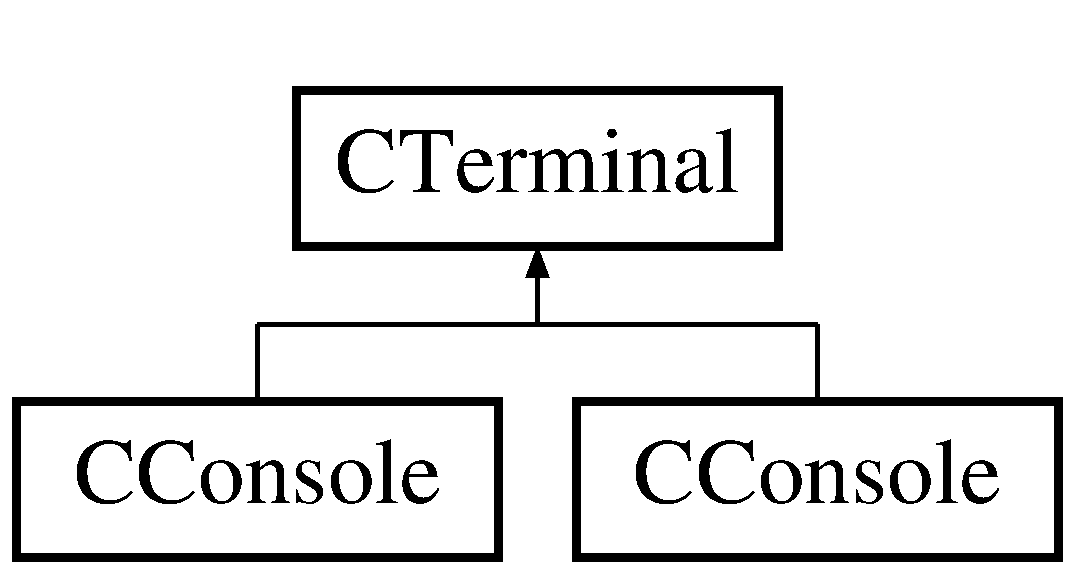
\includegraphics[height=2.000000cm]{class_c_terminal}
\end{center}
\end{figure}
\subsection*{Public Member Functions}
\begin{DoxyCompactItemize}
\item 
\mbox{\Hypertarget{class_c_terminal_a1dc0bbb40f1430d4e23ae079e86cace9}\label{class_c_terminal_a1dc0bbb40f1430d4e23ae079e86cace9}} 
\mbox{\hyperlink{class_c_terminal_a1dc0bbb40f1430d4e23ae079e86cace9}{C\+Terminal}} ()
\begin{DoxyCompactList}\small\item\em Class constructor. \end{DoxyCompactList}\item 
\mbox{\Hypertarget{class_c_terminal_a3f56f1867a20c9d0b3c445be02eea571}\label{class_c_terminal_a3f56f1867a20c9d0b3c445be02eea571}} 
\mbox{\hyperlink{class_c_terminal_a3f56f1867a20c9d0b3c445be02eea571}{$\sim$\+C\+Terminal}} ()
\begin{DoxyCompactList}\small\item\em Class destructor. \end{DoxyCompactList}\end{DoxyCompactItemize}


\subsection{Detailed Description}
System\textquotesingle{}s Terminal class implementation. 

This class implements the virtual methods to access the terminal. 

Definition at line 33 of file T\+E\+R\+M\+I\+N\+A\+L.\+h.



The documentation for this class was generated from the following files\+:\begin{DoxyCompactItemize}
\item 
C\+:/\+Users/\+User/\+Dropbox/\+U\+F\+S\+C/2018.\+2/\+O\+O/\+Projeto\+\_\+\+Final/fw/src/\mbox{\hyperlink{_t_e_r_m_i_n_a_l_8h}{T\+E\+R\+M\+I\+N\+A\+L.\+h}}\item 
C\+:/\+Users/\+User/\+Dropbox/\+U\+F\+S\+C/2018.\+2/\+O\+O/\+Projeto\+\_\+\+Final/fw/src/\mbox{\hyperlink{_t_e_r_m_i_n_a_l_8cpp}{T\+E\+R\+M\+I\+N\+A\+L.\+cpp}}\end{DoxyCompactItemize}

\hypertarget{class_ctime}{}\section{Ctime Class Reference}
\label{class_ctime}\index{Ctime@{Ctime}}


UC\textquotesingle{}s \mbox{\hyperlink{class_ctime}{Ctime}} class implementation.  




{\ttfamily \#include $<$R\+T\+C\+\_\+\+U\+C.\+h$>$}



\subsection{Detailed Description}
UC\textquotesingle{}s \mbox{\hyperlink{class_ctime}{Ctime}} class implementation. 

This class implements the methods to initialize and access a system clock. 

The documentation for this class was generated from the following file\+:\begin{DoxyCompactItemize}
\item 
C\+:/\+Users/\+User/\+Dropbox/\+U\+F\+S\+C/2018.\+2/\+O\+O/\+Projeto\+\_\+\+Final/fw/src/\mbox{\hyperlink{_r_t_c___u_c_8h}{R\+T\+C\+\_\+\+U\+C.\+h}}\end{DoxyCompactItemize}

\hypertarget{classnode}{}\section{node Class Reference}
\label{classnode}\index{node@{node}}


Template of a generic node.  




{\ttfamily \#include $<$node.\+hpp$>$}



\subsection{Detailed Description}
Template of a generic node. 

This class defines a node to be used in double linked data structures. 

The documentation for this class was generated from the following file\+:\begin{DoxyCompactItemize}
\item 
C\+:/\+Users/\+User/\+Dropbox/\+U\+F\+S\+C/2018.\+2/\+O\+O/\+Projeto\+\_\+\+Final/fw/src/\mbox{\hyperlink{node_8hpp}{node.\+hpp}}\end{DoxyCompactItemize}

\chapter{File Documentation}
\hypertarget{_c_o_n_s_o_l_e___p_c_8cpp}{}\section{C\+:/\+Users/\+User/\+Dropbox/\+U\+F\+S\+C/2018.2/\+O\+O/\+Projeto\+\_\+\+Final/fw/src/\+C\+O\+N\+S\+O\+L\+E\+\_\+\+PC.cpp File Reference}
\label{_c_o_n_s_o_l_e___p_c_8cpp}\index{C\+:/\+Users/\+User/\+Dropbox/\+U\+F\+S\+C/2018.\+2/\+O\+O/\+Projeto\+\_\+\+Final/fw/src/\+C\+O\+N\+S\+O\+L\+E\+\_\+\+P\+C.\+cpp@{C\+:/\+Users/\+User/\+Dropbox/\+U\+F\+S\+C/2018.\+2/\+O\+O/\+Projeto\+\_\+\+Final/fw/src/\+C\+O\+N\+S\+O\+L\+E\+\_\+\+P\+C.\+cpp}}


Implements the methods of the \mbox{\hyperlink{class_c_console}{C\+Console}} class.  


{\ttfamily \#include \char`\"{}C\+O\+N\+S\+O\+L\+E\+\_\+\+P\+C.\+h\char`\"{}}\newline
{\ttfamily \#include $<$iostream$>$}\newline
{\ttfamily \#include $<$conio.\+h$>$}\newline
{\ttfamily \#include $<$windows.\+h$>$}\newline


\subsection{Detailed Description}
Implements the methods of the \mbox{\hyperlink{class_c_console}{C\+Console}} class. 

\begin{DoxyVersion}{Version}
1.\+0 
\end{DoxyVersion}
\begin{DoxyAuthor}{Author}
Kleber Gouveia 
\end{DoxyAuthor}
\begin{DoxyDate}{Date}
Nov 25, 2018
\end{DoxyDate}
Module Name\+: \mbox{\hyperlink{_c_o_n_s_o_l_e___p_c_8cpp}{C\+O\+N\+S\+O\+L\+E\+\_\+\+P\+C.\+cpp}}\hypertarget{_u_a_r_t___u_c_8h_References}{}\subsection{References}\label{_u_a_r_t___u_c_8h_References}
\hypertarget{_u_a_r_t___u_c_8h_Revisions}{}\subsection{Revisions}\label{_u_a_r_t___u_c_8h_Revisions}
Revision\+: 1.\+0 25-\/\+Nov-\/2018 Kleber Gouveia
\begin{DoxyItemize}
\item Working baseline. 
\end{DoxyItemize}
\hypertarget{_c_o_n_s_o_l_e___p_c_8h}{}\section{C\+:/\+Users/\+User/\+Dropbox/\+U\+F\+S\+C/2018.2/\+O\+O/\+Projeto\+\_\+\+Final/fw/src/\+C\+O\+N\+S\+O\+L\+E\+\_\+\+PC.h File Reference}
\label{_c_o_n_s_o_l_e___p_c_8h}\index{C\+:/\+Users/\+User/\+Dropbox/\+U\+F\+S\+C/2018.\+2/\+O\+O/\+Projeto\+\_\+\+Final/fw/src/\+C\+O\+N\+S\+O\+L\+E\+\_\+\+P\+C.\+h@{C\+:/\+Users/\+User/\+Dropbox/\+U\+F\+S\+C/2018.\+2/\+O\+O/\+Projeto\+\_\+\+Final/fw/src/\+C\+O\+N\+S\+O\+L\+E\+\_\+\+P\+C.\+h}}


Define the class \mbox{\hyperlink{class_c_console}{C\+Console}} to send log information and receive commands.  


{\ttfamily \#include \char`\"{}T\+E\+R\+M\+I\+N\+A\+L.\+h\char`\"{}}\newline
{\ttfamily \#include \char`\"{}T\+I\+M\+E\+\_\+\+P\+C.\+h\char`\"{}}\newline
\subsection*{Classes}
\begin{DoxyCompactItemize}
\item 
class \mbox{\hyperlink{class_c_console}{C\+Console}}
\begin{DoxyCompactList}\small\item\em PC\textquotesingle{}s \mbox{\hyperlink{class_c_console}{C\+Console}} class implementation. \end{DoxyCompactList}\end{DoxyCompactItemize}


\subsection{Detailed Description}
Define the class \mbox{\hyperlink{class_c_console}{C\+Console}} to send log information and receive commands. 

\begin{DoxyVersion}{Version}
1.\+0 
\end{DoxyVersion}
\begin{DoxyAuthor}{Author}
Kleber Gouveia 
\end{DoxyAuthor}
\begin{DoxyDate}{Date}
Nov 25, 2018
\end{DoxyDate}
Module Name\+: \mbox{\hyperlink{_c_o_n_s_o_l_e___p_c_8h}{C\+O\+N\+S\+O\+L\+E\+\_\+\+P\+C.\+h}}\hypertarget{_u_a_r_t___u_c_8h_References}{}\subsection{References}\label{_u_a_r_t___u_c_8h_References}
\hypertarget{_u_a_r_t___u_c_8h_Revisions}{}\subsection{Revisions}\label{_u_a_r_t___u_c_8h_Revisions}
Revision\+: 1.\+0 25-\/\+Nov-\/2018 Kleber Gouveia
\begin{DoxyItemize}
\item Working baseline. 
\end{DoxyItemize}
\hypertarget{_c_o_n_t_r_o_l_8cpp}{}\section{C\+:/\+Users/\+User/\+Dropbox/\+U\+F\+S\+C/2018.2/\+O\+O/\+Projeto\+\_\+\+Final/fw/src/\+C\+O\+N\+T\+R\+OL.cpp File Reference}
\label{_c_o_n_t_r_o_l_8cpp}\index{C\+:/\+Users/\+User/\+Dropbox/\+U\+F\+S\+C/2018.\+2/\+O\+O/\+Projeto\+\_\+\+Final/fw/src/\+C\+O\+N\+T\+R\+O\+L.\+cpp@{C\+:/\+Users/\+User/\+Dropbox/\+U\+F\+S\+C/2018.\+2/\+O\+O/\+Projeto\+\_\+\+Final/fw/src/\+C\+O\+N\+T\+R\+O\+L.\+cpp}}


Implements the methods of the \mbox{\hyperlink{class_c_control}{C\+Control}} class.  


{\ttfamily \#include \char`\"{}C\+O\+N\+T\+R\+O\+L.\+h\char`\"{}}\newline
{\ttfamily \#include $<$string$>$}\newline


\subsection{Detailed Description}
Implements the methods of the \mbox{\hyperlink{class_c_control}{C\+Control}} class. 

\begin{DoxyVersion}{Version}
1.\+0 
\end{DoxyVersion}
\begin{DoxyAuthor}{Author}
Kleber Gouveia 
\end{DoxyAuthor}
\begin{DoxyDate}{Date}
Nov 28, 2018
\end{DoxyDate}
Module Name\+: C\+O\+N\+T\+R\+O\+L.\+pp\hypertarget{_u_a_r_t___u_c_8h_References}{}\subsection{References}\label{_u_a_r_t___u_c_8h_References}
\hypertarget{_u_a_r_t___u_c_8h_Revisions}{}\subsection{Revisions}\label{_u_a_r_t___u_c_8h_Revisions}
Revision\+: 1.\+0 28-\/\+Nov-\/2018 Kleber Gouveia
\begin{DoxyItemize}
\item Working baseline. 
\end{DoxyItemize}
\hypertarget{_c_o_n_t_r_o_l_8h}{}\section{C\+:/\+Users/\+User/\+Dropbox/\+U\+F\+S\+C/2018.2/\+O\+O/\+Projeto\+\_\+\+Final/fw/src/\+C\+O\+N\+T\+R\+OL.h File Reference}
\label{_c_o_n_t_r_o_l_8h}\index{C\+:/\+Users/\+User/\+Dropbox/\+U\+F\+S\+C/2018.\+2/\+O\+O/\+Projeto\+\_\+\+Final/fw/src/\+C\+O\+N\+T\+R\+O\+L.\+h@{C\+:/\+Users/\+User/\+Dropbox/\+U\+F\+S\+C/2018.\+2/\+O\+O/\+Projeto\+\_\+\+Final/fw/src/\+C\+O\+N\+T\+R\+O\+L.\+h}}


Define the class \mbox{\hyperlink{class_c_control}{C\+Control}} that manages the logic to put messages in the display and the console.  


{\ttfamily \#include \char`\"{}queue.\+hpp\char`\"{}}\newline
\subsection*{Classes}
\begin{DoxyCompactItemize}
\item 
class \mbox{\hyperlink{class_c_control}{C\+Control}}
\begin{DoxyCompactList}\small\item\em \mbox{\hyperlink{class_c_control}{C\+Control}} class implementation. \end{DoxyCompactList}\end{DoxyCompactItemize}
\subsection*{Macros}
\begin{DoxyCompactItemize}
\item 
\#define \mbox{\hyperlink{_c_o_n_t_r_o_l_8h_a13ed95a02e5cd9d2e22c42402f587422}{T\+I\+M\+E\+\_\+\+D\+U\+R\+A\+T\+I\+O\+N\+\_\+\+A\+D\+\_\+\+M\+SG}}~3000 /$\ast$$\ast$duration of advertising messages shown on diaplay is miliseconds$\ast$/
\end{DoxyCompactItemize}


\subsection{Detailed Description}
Define the class \mbox{\hyperlink{class_c_control}{C\+Control}} that manages the logic to put messages in the display and the console. 

\begin{DoxyVersion}{Version}
1.\+0 
\end{DoxyVersion}
\begin{DoxyAuthor}{Author}
Kleber Gouveia 
\end{DoxyAuthor}
\begin{DoxyDate}{Date}
Nov 28, 2018
\end{DoxyDate}
Module Name\+: \mbox{\hyperlink{_c_o_n_t_r_o_l_8h}{C\+O\+N\+T\+R\+O\+L.\+h}}\hypertarget{_u_a_r_t___u_c_8h_References}{}\subsection{References}\label{_u_a_r_t___u_c_8h_References}
\hypertarget{_u_a_r_t___u_c_8h_Revisions}{}\subsection{Revisions}\label{_u_a_r_t___u_c_8h_Revisions}
Revision\+: 1.\+0 28-\/\+Nov-\/2018 Kleber Gouveia
\begin{DoxyItemize}
\item Working baseline. 
\end{DoxyItemize}

\subsection{Macro Definition Documentation}
\mbox{\Hypertarget{_c_o_n_t_r_o_l_8h_a13ed95a02e5cd9d2e22c42402f587422}\label{_c_o_n_t_r_o_l_8h_a13ed95a02e5cd9d2e22c42402f587422}} 
\index{C\+O\+N\+T\+R\+O\+L.\+h@{C\+O\+N\+T\+R\+O\+L.\+h}!T\+I\+M\+E\+\_\+\+D\+U\+R\+A\+T\+I\+O\+N\+\_\+\+A\+D\+\_\+\+M\+SG@{T\+I\+M\+E\+\_\+\+D\+U\+R\+A\+T\+I\+O\+N\+\_\+\+A\+D\+\_\+\+M\+SG}}
\index{T\+I\+M\+E\+\_\+\+D\+U\+R\+A\+T\+I\+O\+N\+\_\+\+A\+D\+\_\+\+M\+SG@{T\+I\+M\+E\+\_\+\+D\+U\+R\+A\+T\+I\+O\+N\+\_\+\+A\+D\+\_\+\+M\+SG}!C\+O\+N\+T\+R\+O\+L.\+h@{C\+O\+N\+T\+R\+O\+L.\+h}}
\subsubsection{\texorpdfstring{T\+I\+M\+E\+\_\+\+D\+U\+R\+A\+T\+I\+O\+N\+\_\+\+A\+D\+\_\+\+M\+SG}{TIME\_DURATION\_AD\_MSG}}
{\footnotesize\ttfamily \#define T\+I\+M\+E\+\_\+\+D\+U\+R\+A\+T\+I\+O\+N\+\_\+\+A\+D\+\_\+\+M\+SG~3000 /$\ast$$\ast$duration of advertising messages shown on diaplay is miliseconds$\ast$/}

Mechanism to select the hardware platform to run 

Definition at line 41 of file C\+O\+N\+T\+R\+O\+L.\+h.


\hypertarget{_d_a_t_e___t_i_m_e_8cpp}{}\section{C\+:/\+Users/\+User/\+Dropbox/\+U\+F\+S\+C/2018.2/\+O\+O/\+Projeto\+\_\+\+Final/fw/src/\+D\+A\+T\+E\+\_\+\+T\+I\+ME.cpp File Reference}
\label{_d_a_t_e___t_i_m_e_8cpp}\index{C\+:/\+Users/\+User/\+Dropbox/\+U\+F\+S\+C/2018.\+2/\+O\+O/\+Projeto\+\_\+\+Final/fw/src/\+D\+A\+T\+E\+\_\+\+T\+I\+M\+E.\+cpp@{C\+:/\+Users/\+User/\+Dropbox/\+U\+F\+S\+C/2018.\+2/\+O\+O/\+Projeto\+\_\+\+Final/fw/src/\+D\+A\+T\+E\+\_\+\+T\+I\+M\+E.\+cpp}}


Implements the methods of the \mbox{\hyperlink{class_c_date_time}{C\+Date\+Time}} class.  


{\ttfamily \#include \char`\"{}D\+A\+T\+E\+\_\+\+T\+I\+M\+E.\+h\char`\"{}}\newline


\subsection{Detailed Description}
Implements the methods of the \mbox{\hyperlink{class_c_date_time}{C\+Date\+Time}} class. 

\begin{DoxyVersion}{Version}
1.\+0 
\end{DoxyVersion}
\begin{DoxyAuthor}{Author}
Kleber Gouveia 
\end{DoxyAuthor}
\begin{DoxyDate}{Date}
Nov 23, 2018
\end{DoxyDate}
Module Name\+: \mbox{\hyperlink{_d_a_t_e___t_i_m_e_8cpp}{D\+A\+T\+E\+\_\+\+T\+I\+M\+E.\+cpp}}\hypertarget{_u_a_r_t___u_c_8h_References}{}\subsection{References}\label{_u_a_r_t___u_c_8h_References}
\hypertarget{_u_a_r_t___u_c_8h_Revisions}{}\subsection{Revisions}\label{_u_a_r_t___u_c_8h_Revisions}
Revision\+: 1.\+0 23-\/\+Nov-\/2018 Kleber Gouveia
\begin{DoxyItemize}
\item Working baseline. 
\end{DoxyItemize}
\hypertarget{_d_a_t_e___t_i_m_e_8h}{}\section{C\+:/\+Users/\+User/\+Dropbox/\+U\+F\+S\+C/2018.2/\+O\+O/\+Projeto\+\_\+\+Final/fw/src/\+D\+A\+T\+E\+\_\+\+T\+I\+ME.h File Reference}
\label{_d_a_t_e___t_i_m_e_8h}\index{C\+:/\+Users/\+User/\+Dropbox/\+U\+F\+S\+C/2018.\+2/\+O\+O/\+Projeto\+\_\+\+Final/fw/src/\+D\+A\+T\+E\+\_\+\+T\+I\+M\+E.\+h@{C\+:/\+Users/\+User/\+Dropbox/\+U\+F\+S\+C/2018.\+2/\+O\+O/\+Projeto\+\_\+\+Final/fw/src/\+D\+A\+T\+E\+\_\+\+T\+I\+M\+E.\+h}}


Define the class to model the system time.  


{\ttfamily \#include $<$string$>$}\newline
\subsection*{Classes}
\begin{DoxyCompactItemize}
\item 
class \mbox{\hyperlink{class_c_date_time}{C\+Date\+Time}}
\begin{DoxyCompactList}\small\item\em System\textquotesingle{}s \mbox{\hyperlink{class_c_date_time}{C\+Date\+Time}} class implementation. \end{DoxyCompactList}\end{DoxyCompactItemize}


\subsection{Detailed Description}
Define the class to model the system time. 

\begin{DoxyVersion}{Version}
1.\+0 
\end{DoxyVersion}
\begin{DoxyAuthor}{Author}
Kleber Gouveia 
\end{DoxyAuthor}
\begin{DoxyDate}{Date}
Nov 23, 2018
\end{DoxyDate}
Module Name\+: \mbox{\hyperlink{_d_a_t_e___t_i_m_e_8h}{D\+A\+T\+E\+\_\+\+T\+I\+M\+E.\+h}}\hypertarget{_u_a_r_t___u_c_8h_References}{}\subsection{References}\label{_u_a_r_t___u_c_8h_References}
\hypertarget{_u_a_r_t___u_c_8h_Revisions}{}\subsection{Revisions}\label{_u_a_r_t___u_c_8h_Revisions}
Revision\+: 1.\+0 23-\/\+Nov-\/2018 Kleber Gouveia
\begin{DoxyItemize}
\item Working baseline. 
\end{DoxyItemize}
\hypertarget{_d_i_s_p_l_a_y_8h}{}\section{C\+:/\+Users/\+User/\+Dropbox/\+U\+F\+S\+C/2018.2/\+O\+O/\+Projeto\+\_\+\+Final/fw/src/\+D\+I\+S\+P\+L\+AY.h File Reference}
\label{_d_i_s_p_l_a_y_8h}\index{C\+:/\+Users/\+User/\+Dropbox/\+U\+F\+S\+C/2018.\+2/\+O\+O/\+Projeto\+\_\+\+Final/fw/src/\+D\+I\+S\+P\+L\+A\+Y.\+h@{C\+:/\+Users/\+User/\+Dropbox/\+U\+F\+S\+C/2018.\+2/\+O\+O/\+Projeto\+\_\+\+Final/fw/src/\+D\+I\+S\+P\+L\+A\+Y.\+h}}


Define the class to model the display interface.  


{\ttfamily \#include $<$string$>$}\newline
\subsection*{Classes}
\begin{DoxyCompactItemize}
\item 
class \mbox{\hyperlink{class_c_display}{C\+Display}}
\begin{DoxyCompactList}\small\item\em System\textquotesingle{}s Display class implementation. \end{DoxyCompactList}\end{DoxyCompactItemize}


\subsection{Detailed Description}
Define the class to model the display interface. 

\begin{DoxyVersion}{Version}
1.\+0 
\end{DoxyVersion}
\begin{DoxyAuthor}{Author}
Kleber Gouveia 
\end{DoxyAuthor}
\begin{DoxyDate}{Date}
Nov 22, 2018
\end{DoxyDate}
Module Name\+: \mbox{\hyperlink{_d_i_s_p_l_a_y_8h}{D\+I\+S\+P\+L\+A\+Y.\+h}}\hypertarget{_u_a_r_t___u_c_8h_References}{}\subsection{References}\label{_u_a_r_t___u_c_8h_References}
\hypertarget{_u_a_r_t___u_c_8h_Revisions}{}\subsection{Revisions}\label{_u_a_r_t___u_c_8h_Revisions}
Revision\+: 1.\+0 22-\/\+Nov-\/2018 Kleber Gouveia
\begin{DoxyItemize}
\item Working baseline. 
\end{DoxyItemize}
\hypertarget{_f_s_m_8h}{}\section{C\+:/\+Users/\+User/\+Dropbox/\+U\+F\+S\+C/2018.2/\+O\+O/\+Projeto\+\_\+\+Final/fw/src/\+F\+SM.h File Reference}
\label{_f_s_m_8h}\index{C\+:/\+Users/\+User/\+Dropbox/\+U\+F\+S\+C/2018.\+2/\+O\+O/\+Projeto\+\_\+\+Final/fw/src/\+F\+S\+M.\+h@{C\+:/\+Users/\+User/\+Dropbox/\+U\+F\+S\+C/2018.\+2/\+O\+O/\+Projeto\+\_\+\+Final/fw/src/\+F\+S\+M.\+h}}


Implements the methods of the \mbox{\hyperlink{class_c_f_s_m}{C\+F\+SM}} class.  


{\ttfamily \#include $<$string$>$}\newline
\subsection*{Classes}
\begin{DoxyCompactItemize}
\item 
class \mbox{\hyperlink{class_c_f_s_m}{C\+F\+SM}}
\begin{DoxyCompactList}\small\item\em System\textquotesingle{}s \mbox{\hyperlink{class_c_f_s_m}{C\+F\+SM}} class implementation. \end{DoxyCompactList}\end{DoxyCompactItemize}
\subsection*{Typedefs}
\begin{DoxyCompactItemize}
\item 
typedef enum \mbox{\hyperlink{_f_s_m_8h_ac2ba3a71cf64ee5edad4978c6fddd410}{F\+S\+Mstate}} \mbox{\hyperlink{_f_s_m_8h_a7d59fd39d0fd81e92c4d689f0f6e1fab}{F\+S\+Mstate\+\_\+t}}
\end{DoxyCompactItemize}
\subsection*{Enumerations}
\begin{DoxyCompactItemize}
\item 
enum \mbox{\hyperlink{_f_s_m_8h_ac2ba3a71cf64ee5edad4978c6fddd410}{F\+S\+Mstate}} 
\end{DoxyCompactItemize}


\subsection{Detailed Description}
Implements the methods of the \mbox{\hyperlink{class_c_f_s_m}{C\+F\+SM}} class. 

Define the class to control the finite machine state of the vending machine.

\begin{DoxyVersion}{Version}
1.\+0 
\end{DoxyVersion}
\begin{DoxyAuthor}{Author}
Kleber Gouveia 
\end{DoxyAuthor}
\begin{DoxyDate}{Date}
Nov 10, 2018
\end{DoxyDate}
Module Name\+: \mbox{\hyperlink{_f_s_m_8h}{F\+S\+M.\+h}}\hypertarget{_u_a_r_t___u_c_8h_References}{}\subsection{References}\label{_u_a_r_t___u_c_8h_References}
\hypertarget{_u_a_r_t___u_c_8h_Revisions}{}\subsection{Revisions}\label{_u_a_r_t___u_c_8h_Revisions}
Revision\+: 1.\+0 10-\/\+Nov-\/2018 Kleber Gouveia
\begin{DoxyItemize}
\item Working baseline. 
\end{DoxyItemize}

\subsection{Typedef Documentation}
\mbox{\Hypertarget{_f_s_m_8h_a7d59fd39d0fd81e92c4d689f0f6e1fab}\label{_f_s_m_8h_a7d59fd39d0fd81e92c4d689f0f6e1fab}} 
\index{F\+S\+M.\+h@{F\+S\+M.\+h}!F\+S\+Mstate\+\_\+t@{F\+S\+Mstate\+\_\+t}}
\index{F\+S\+Mstate\+\_\+t@{F\+S\+Mstate\+\_\+t}!F\+S\+M.\+h@{F\+S\+M.\+h}}
\subsubsection{\texorpdfstring{F\+S\+Mstate\+\_\+t}{FSMstate\_t}}
{\footnotesize\ttfamily typedef enum \mbox{\hyperlink{_f_s_m_8h_ac2ba3a71cf64ee5edad4978c6fddd410}{F\+S\+Mstate}}  \mbox{\hyperlink{_f_s_m_8h_a7d59fd39d0fd81e92c4d689f0f6e1fab}{F\+S\+Mstate\+\_\+t}}}

Data type of the machine states 

\subsection{Enumeration Type Documentation}
\mbox{\Hypertarget{_f_s_m_8h_ac2ba3a71cf64ee5edad4978c6fddd410}\label{_f_s_m_8h_ac2ba3a71cf64ee5edad4978c6fddd410}} 
\index{F\+S\+M.\+h@{F\+S\+M.\+h}!F\+S\+Mstate@{F\+S\+Mstate}}
\index{F\+S\+Mstate@{F\+S\+Mstate}!F\+S\+M.\+h@{F\+S\+M.\+h}}
\subsubsection{\texorpdfstring{F\+S\+Mstate}{FSMstate}}
{\footnotesize\ttfamily enum \mbox{\hyperlink{_f_s_m_8h_ac2ba3a71cf64ee5edad4978c6fddd410}{F\+S\+Mstate}}}

Data type of the machine states 

Definition at line 37 of file F\+S\+M.\+h.


\hypertarget{_g_p_i_o___p_c_8h}{}\section{C\+:/\+Users/\+User/\+Dropbox/\+U\+F\+S\+C/2018.2/\+O\+O/\+Projeto\+\_\+\+Final/fw/src/\+G\+P\+I\+O\+\_\+\+PC.h File Reference}
\label{_g_p_i_o___p_c_8h}\index{C\+:/\+Users/\+User/\+Dropbox/\+U\+F\+S\+C/2018.\+2/\+O\+O/\+Projeto\+\_\+\+Final/fw/src/\+G\+P\+I\+O\+\_\+\+P\+C.\+h@{C\+:/\+Users/\+User/\+Dropbox/\+U\+F\+S\+C/2018.\+2/\+O\+O/\+Projeto\+\_\+\+Final/fw/src/\+G\+P\+I\+O\+\_\+\+P\+C.\+h}}


Implements the methods of the \mbox{\hyperlink{class_c_g_p_i_o}{C\+G\+P\+IO}} class.  


{\ttfamily \#include \char`\"{}I\+O.\+h\char`\"{}}\newline
\subsection*{Classes}
\begin{DoxyCompactItemize}
\item 
class \mbox{\hyperlink{class_c_g_p_i_o}{C\+G\+P\+IO}}
\begin{DoxyCompactList}\small\item\em PC\textquotesingle{}s \mbox{\hyperlink{class_c_g_p_i_o}{C\+G\+P\+IO}} class implementation. \end{DoxyCompactList}\end{DoxyCompactItemize}


\subsection{Detailed Description}
Implements the methods of the \mbox{\hyperlink{class_c_g_p_i_o}{C\+G\+P\+IO}} class. 

Define the class for access the PC\textquotesingle{}s I\+Os.

\begin{DoxyVersion}{Version}
1.\+0 
\end{DoxyVersion}
\begin{DoxyAuthor}{Author}
Kleber Gouveia 
\end{DoxyAuthor}
\begin{DoxyDate}{Date}
Nov 10, 2018
\end{DoxyDate}
Module Name\+: \mbox{\hyperlink{_g_p_i_o___p_c_8h}{G\+P\+I\+O\+\_\+\+P\+C.\+h}}\hypertarget{_u_a_r_t___u_c_8h_References}{}\subsection{References}\label{_u_a_r_t___u_c_8h_References}
\hypertarget{_u_a_r_t___u_c_8h_Revisions}{}\subsection{Revisions}\label{_u_a_r_t___u_c_8h_Revisions}
Revision\+: 1.\+0 10-\/\+Nov-\/2018 Kleber Gouveia
\begin{DoxyItemize}
\item Working baseline. 
\end{DoxyItemize}
\hypertarget{_g_p_i_o___u_c_8cpp}{}\section{C\+:/\+Users/\+User/\+Dropbox/\+U\+F\+S\+C/2018.2/\+O\+O/\+Projeto\+\_\+\+Final/fw/src/\+G\+P\+I\+O\+\_\+\+UC.cpp File Reference}
\label{_g_p_i_o___u_c_8cpp}\index{C\+:/\+Users/\+User/\+Dropbox/\+U\+F\+S\+C/2018.\+2/\+O\+O/\+Projeto\+\_\+\+Final/fw/src/\+G\+P\+I\+O\+\_\+\+U\+C.\+cpp@{C\+:/\+Users/\+User/\+Dropbox/\+U\+F\+S\+C/2018.\+2/\+O\+O/\+Projeto\+\_\+\+Final/fw/src/\+G\+P\+I\+O\+\_\+\+U\+C.\+cpp}}


Implements the methods of the \mbox{\hyperlink{class_c_g_p_i_o}{C\+G\+P\+IO}} class.  


{\ttfamily \#include \char`\"{}G\+P\+I\+O\+\_\+\+U\+C.\+h\char`\"{}}\newline
{\ttfamily \#include \char`\"{}driverlib/gpio.\+h\char`\"{}}\newline
{\ttfamily \#include \char`\"{}driverlib/sysctl.\+h\char`\"{}}\newline
{\ttfamily \#include \char`\"{}inc/hw\+\_\+memmap.\+h\char`\"{}}\newline
{\ttfamily \#include \char`\"{}inc/hw\+\_\+gpio.\+h\char`\"{}}\newline
{\ttfamily \#include \char`\"{}inc/hw\+\_\+types.\+h\char`\"{}}\newline
\subsection*{Functions}
\begin{DoxyCompactItemize}
\item 
void \mbox{\hyperlink{_g_p_i_o___u_c_8cpp_a1f5d1820cabbff7f390eaa31ee8b98aa}{G\+P\+I\+O\+I\+SR}} (void)
\begin{DoxyCompactList}\small\item\em friend function that performs the I\+SR treatment to read the inputs. \end{DoxyCompactList}\end{DoxyCompactItemize}


\subsection{Detailed Description}
Implements the methods of the \mbox{\hyperlink{class_c_g_p_i_o}{C\+G\+P\+IO}} class. 

\begin{DoxyVersion}{Version}
1.\+0 
\end{DoxyVersion}
\begin{DoxyAuthor}{Author}
Kleber Gouveia 
\end{DoxyAuthor}
\begin{DoxyDate}{Date}
Nov 10, 2018
\end{DoxyDate}
Module Name\+: \mbox{\hyperlink{_g_p_i_o___u_c_8cpp}{G\+P\+I\+O\+\_\+\+U\+C.\+cpp}}\hypertarget{_u_a_r_t___u_c_8h_References}{}\subsection{References}\label{_u_a_r_t___u_c_8h_References}
\hypertarget{_u_a_r_t___u_c_8h_Revisions}{}\subsection{Revisions}\label{_u_a_r_t___u_c_8h_Revisions}
Revision\+: 1.\+0 10-\/\+Nov-\/2018 Kleber Gouveia
\begin{DoxyItemize}
\item Working baseline. 
\end{DoxyItemize}

\subsection{Function Documentation}
\mbox{\Hypertarget{_g_p_i_o___u_c_8cpp_a1f5d1820cabbff7f390eaa31ee8b98aa}\label{_g_p_i_o___u_c_8cpp_a1f5d1820cabbff7f390eaa31ee8b98aa}} 
\index{G\+P\+I\+O\+\_\+\+U\+C.\+cpp@{G\+P\+I\+O\+\_\+\+U\+C.\+cpp}!G\+P\+I\+O\+I\+SR@{G\+P\+I\+O\+I\+SR}}
\index{G\+P\+I\+O\+I\+SR@{G\+P\+I\+O\+I\+SR}!G\+P\+I\+O\+\_\+\+U\+C.\+cpp@{G\+P\+I\+O\+\_\+\+U\+C.\+cpp}}
\subsubsection{\texorpdfstring{G\+P\+I\+O\+I\+S\+R()}{GPIOISR()}}
{\footnotesize\ttfamily void G\+P\+I\+O\+I\+SR (\begin{DoxyParamCaption}\item[{void}]{ }\end{DoxyParamCaption})}



friend function that performs the I\+SR treatment to read the inputs. 


\begin{DoxyParams}{Parameters}
{\em none} & \\
\hline
\end{DoxyParams}
\begin{DoxyReturn}{Returns}
none 
\end{DoxyReturn}


Definition at line 202 of file G\+P\+I\+O\+\_\+\+U\+C.\+cpp.


\hypertarget{_g_p_i_o___u_c_8h}{}\section{C\+:/\+Users/\+User/\+Dropbox/\+U\+F\+S\+C/2018.2/\+O\+O/\+Projeto\+\_\+\+Final/fw/src/\+G\+P\+I\+O\+\_\+\+UC.h File Reference}
\label{_g_p_i_o___u_c_8h}\index{C\+:/\+Users/\+User/\+Dropbox/\+U\+F\+S\+C/2018.\+2/\+O\+O/\+Projeto\+\_\+\+Final/fw/src/\+G\+P\+I\+O\+\_\+\+U\+C.\+h@{C\+:/\+Users/\+User/\+Dropbox/\+U\+F\+S\+C/2018.\+2/\+O\+O/\+Projeto\+\_\+\+Final/fw/src/\+G\+P\+I\+O\+\_\+\+U\+C.\+h}}


Define the class for access the microncontroller\textquotesingle{}s I\+Os.  


{\ttfamily \#include \char`\"{}I\+O.\+h\char`\"{}}\newline
\subsection*{Classes}
\begin{DoxyCompactItemize}
\item 
class \mbox{\hyperlink{class_g_p_i_o___u_c}{G\+P\+I\+O\+\_\+\+UC}}
\begin{DoxyCompactList}\small\item\em uC\textquotesingle{}s G\+P\+IO implementation. \end{DoxyCompactList}\end{DoxyCompactItemize}


\subsection{Detailed Description}
Define the class for access the microncontroller\textquotesingle{}s I\+Os. 

\begin{DoxyVersion}{Version}
1.\+0 
\end{DoxyVersion}
\begin{DoxyAuthor}{Author}
Kleber Gouveia 
\end{DoxyAuthor}
\begin{DoxyDate}{Date}
Nov 10, 2018
\end{DoxyDate}
Module Name\+: \mbox{\hyperlink{_g_p_i_o___u_c_8h}{G\+P\+I\+O\+\_\+\+U\+C.\+h}}\hypertarget{main_8cpp_References}{}\subsection{References}\label{main_8cpp_References}
\hypertarget{_g_p_i_o___u_c_8h_Revisions}{}\subsection{Revisions}\label{_g_p_i_o___u_c_8h_Revisions}
Revision\+: 1.\+0 10-\/\+Nov-\/2018 Kleber Gouveia
\begin{DoxyItemize}
\item Working baseline. 
\end{DoxyItemize}
\hypertarget{_i_o_8cpp}{}\section{C\+:/\+Users/\+User/\+Dropbox/\+U\+F\+S\+C/2018.2/\+O\+O/\+Projeto\+\_\+\+Final/fw/src/\+IO.cpp File Reference}
\label{_i_o_8cpp}\index{C\+:/\+Users/\+User/\+Dropbox/\+U\+F\+S\+C/2018.\+2/\+O\+O/\+Projeto\+\_\+\+Final/fw/src/\+I\+O.\+cpp@{C\+:/\+Users/\+User/\+Dropbox/\+U\+F\+S\+C/2018.\+2/\+O\+O/\+Projeto\+\_\+\+Final/fw/src/\+I\+O.\+cpp}}


Define the class to model the IO interface.  


{\ttfamily \#include \char`\"{}I\+O.\+h\char`\"{}}\newline


\subsection{Detailed Description}
Define the class to model the IO interface. 

\begin{DoxyVersion}{Version}
1.\+0 
\end{DoxyVersion}
\begin{DoxyAuthor}{Author}
Kleber Gouveia 
\end{DoxyAuthor}
\begin{DoxyDate}{Date}
Nov 10, 2018
\end{DoxyDate}
Module Name\+: \mbox{\hyperlink{_i_o_8cpp}{I\+O.\+cpp}}\hypertarget{_u_a_r_t___u_c_8h_References}{}\subsection{References}\label{_u_a_r_t___u_c_8h_References}
\hypertarget{_u_a_r_t___u_c_8h_Revisions}{}\subsection{Revisions}\label{_u_a_r_t___u_c_8h_Revisions}
Revision\+: 1.\+0 10-\/\+Nov-\/2018 Kleber Gouveia
\begin{DoxyItemize}
\item Working baseline. 
\end{DoxyItemize}
\hypertarget{_i_o_8h}{}\section{C\+:/\+Users/\+User/\+Dropbox/\+U\+F\+S\+C/2018.2/\+O\+O/\+Projeto\+\_\+\+Final/fw/src/\+IO.h File Reference}
\label{_i_o_8h}\index{C\+:/\+Users/\+User/\+Dropbox/\+U\+F\+S\+C/2018.\+2/\+O\+O/\+Projeto\+\_\+\+Final/fw/src/\+I\+O.\+h@{C\+:/\+Users/\+User/\+Dropbox/\+U\+F\+S\+C/2018.\+2/\+O\+O/\+Projeto\+\_\+\+Final/fw/src/\+I\+O.\+h}}


Defini��o da classe de acesso a interface de entrada e s�ida do sistema.  


\subsection*{Macros}
\begin{DoxyCompactItemize}
\item 
\#define \mbox{\hyperlink{_i_o_8h_ad289413cf5936a0c0c2a46d2d9aab03b}{M025}}~0x01
\item 
\#define \mbox{\hyperlink{_i_o_8h_a03058f38ccb7bdf6825fe20aff7dec68}{M050}}~0x02
\item 
\#define \mbox{\hyperlink{_i_o_8h_a992643b5ff82c3cc4b5f6609da7d2547}{M100}}~0x04
\item 
\#define \mbox{\hyperlink{_i_o_8h_a9af8717485817233e79a6039c170e7fe}{M\+E\+ET}}~0x08
\item 
\#define \mbox{\hyperlink{_i_o_8h_a44d040c31822071333f7ea49ce7b743d}{E\+T\+I\+R\+PS}}~0x10
\item 
\#define \mbox{\hyperlink{_i_o_8h_adb08aff46bb7262714b2a36aba398c9d}{D\+EV}}~0x20
\end{DoxyCompactItemize}


\subsection{Detailed Description}
Defini��o da classe de acesso a interface de entrada e s�ida do sistema. 

\begin{DoxyAuthor}{Author}
Kleber Gouveia 
\end{DoxyAuthor}


\subsection{Macro Definition Documentation}
\mbox{\Hypertarget{_i_o_8h_adb08aff46bb7262714b2a36aba398c9d}\label{_i_o_8h_adb08aff46bb7262714b2a36aba398c9d}} 
\index{I\+O.\+h@{I\+O.\+h}!D\+EV@{D\+EV}}
\index{D\+EV@{D\+EV}!I\+O.\+h@{I\+O.\+h}}
\subsubsection{\texorpdfstring{D\+EV}{DEV}}
{\footnotesize\ttfamily \#define D\+EV~0x20}

Devolucao 

Definition at line 15 of file I\+O.\+h.

\mbox{\Hypertarget{_i_o_8h_a44d040c31822071333f7ea49ce7b743d}\label{_i_o_8h_a44d040c31822071333f7ea49ce7b743d}} 
\index{I\+O.\+h@{I\+O.\+h}!E\+T\+I\+R\+PS@{E\+T\+I\+R\+PS}}
\index{E\+T\+I\+R\+PS@{E\+T\+I\+R\+PS}!I\+O.\+h@{I\+O.\+h}}
\subsubsection{\texorpdfstring{E\+T\+I\+R\+PS}{ETIRPS}}
{\footnotesize\ttfamily \#define E\+T\+I\+R\+PS~0x10}

Refrigerante E\+T\+I\+R\+PS 

Definition at line 14 of file I\+O.\+h.

\mbox{\Hypertarget{_i_o_8h_ad289413cf5936a0c0c2a46d2d9aab03b}\label{_i_o_8h_ad289413cf5936a0c0c2a46d2d9aab03b}} 
\index{I\+O.\+h@{I\+O.\+h}!M025@{M025}}
\index{M025@{M025}!I\+O.\+h@{I\+O.\+h}}
\subsubsection{\texorpdfstring{M025}{M025}}
{\footnotesize\ttfamily \#define M025~0x01}

Moeda de R\$0,25 

Definition at line 10 of file I\+O.\+h.

\mbox{\Hypertarget{_i_o_8h_a03058f38ccb7bdf6825fe20aff7dec68}\label{_i_o_8h_a03058f38ccb7bdf6825fe20aff7dec68}} 
\index{I\+O.\+h@{I\+O.\+h}!M050@{M050}}
\index{M050@{M050}!I\+O.\+h@{I\+O.\+h}}
\subsubsection{\texorpdfstring{M050}{M050}}
{\footnotesize\ttfamily \#define M050~0x02}

Moeda de R\$0,50 

Definition at line 11 of file I\+O.\+h.

\mbox{\Hypertarget{_i_o_8h_a992643b5ff82c3cc4b5f6609da7d2547}\label{_i_o_8h_a992643b5ff82c3cc4b5f6609da7d2547}} 
\index{I\+O.\+h@{I\+O.\+h}!M100@{M100}}
\index{M100@{M100}!I\+O.\+h@{I\+O.\+h}}
\subsubsection{\texorpdfstring{M100}{M100}}
{\footnotesize\ttfamily \#define M100~0x04}

Moeda de R\$1,00 

Definition at line 12 of file I\+O.\+h.

\mbox{\Hypertarget{_i_o_8h_a9af8717485817233e79a6039c170e7fe}\label{_i_o_8h_a9af8717485817233e79a6039c170e7fe}} 
\index{I\+O.\+h@{I\+O.\+h}!M\+E\+ET@{M\+E\+ET}}
\index{M\+E\+ET@{M\+E\+ET}!I\+O.\+h@{I\+O.\+h}}
\subsubsection{\texorpdfstring{M\+E\+ET}{MEET}}
{\footnotesize\ttfamily \#define M\+E\+ET~0x08}

Refrigentante M\+E\+ET 

Definition at line 13 of file I\+O.\+h.


\hypertarget{_l_c_d___n_h_d_c12864_8c}{}\section{C\+:/\+Users/\+User/\+Dropbox/\+U\+F\+S\+C/2018.2/\+O\+O/\+Projeto\+\_\+\+Final/fw/src/\+L\+C\+D\+\_\+\+N\+H\+D\+C12864.c File Reference}
\label{_l_c_d___n_h_d_c12864_8c}\index{C\+:/\+Users/\+User/\+Dropbox/\+U\+F\+S\+C/2018.\+2/\+O\+O/\+Projeto\+\_\+\+Final/fw/src/\+L\+C\+D\+\_\+\+N\+H\+D\+C12864.\+c@{C\+:/\+Users/\+User/\+Dropbox/\+U\+F\+S\+C/2018.\+2/\+O\+O/\+Projeto\+\_\+\+Final/fw/src/\+L\+C\+D\+\_\+\+N\+H\+D\+C12864.\+c}}


Implements the drivers of the L\+CD N\+H\+D\+C1264.  


{\ttfamily \#include $<$stdint.\+h$>$}\newline
{\ttfamily \#include $<$stdbool.\+h$>$}\newline
{\ttfamily \#include \char`\"{}driverlib/gpio.\+h\char`\"{}}\newline
{\ttfamily \#include \char`\"{}L\+C\+D\+\_\+\+N\+H\+D\+C12864.\+h\char`\"{}}\newline
{\ttfamily \#include \char`\"{}driverlib/sysctl.\+h\char`\"{}}\newline
{\ttfamily \#include \char`\"{}inc/hw\+\_\+memmap.\+h\char`\"{}}\newline
\subsection*{Functions}
\begin{DoxyCompactItemize}
\item 
void \mbox{\hyperlink{_l_c_d___n_h_d_c12864_8c_ab4d5ff2177b0c46bd3fe97a229b589a2}{L\+C\+D\+Initialize\+N\+H\+D\+C12864}} (void)
\begin{DoxyCompactList}\small\item\em L\+CD initialization. \end{DoxyCompactList}\item 
void \mbox{\hyperlink{_l_c_d___n_h_d_c12864_8c_a08548aab6d46d9d45e24c071af828712}{L\+C\+D\+Write}} (char mode, char data)
\begin{DoxyCompactList}\small\item\em Function to write data and commands in the L\+CD. \end{DoxyCompactList}\item 
void \mbox{\hyperlink{_l_c_d___n_h_d_c12864_8c_a2dd0f4693e82ac481b90e689cf6dc773}{L\+C\+D\+Set\+Start\+Line}} (char addr)
\begin{DoxyCompactList}\small\item\em Function to read data rom the L\+CD. \end{DoxyCompactList}\item 
void \mbox{\hyperlink{_l_c_d___n_h_d_c12864_8c_aaf860efa873b0dab1001f227eabe9684}{L\+C\+D\+Set\+Column}} (char addr)
\begin{DoxyCompactList}\small\item\em Function to set the column to write. \end{DoxyCompactList}\item 
void \mbox{\hyperlink{_l_c_d___n_h_d_c12864_8c_ad7b46eb2cf7ce871dd24f16d503f992c}{L\+C\+D\+Set\+Page}} (char addr)
\begin{DoxyCompactList}\small\item\em Function to set the page to write. \end{DoxyCompactList}\item 
void \mbox{\hyperlink{_l_c_d___n_h_d_c12864_8c_a3a94c0f44f76db891e66d98966f904e8}{L\+C\+D\+Clear}} (void)
\begin{DoxyCompactList}\small\item\em Function to clear the entire L\+CD. \end{DoxyCompactList}\item 
void \mbox{\hyperlink{_l_c_d___n_h_d_c12864_8c_ac1b6f92b924f05d7a8806da4be747373}{L\+C\+D\+Reverse\+Blink}} (char n\+Blink)
\begin{DoxyCompactList}\small\item\em Function to blink the L\+CD a number of times. \end{DoxyCompactList}\item 
void \mbox{\hyperlink{_l_c_d___n_h_d_c12864_8c_a6ea60b87eaa45cbf02e0fed1b8604f58}{L\+C\+D\+Write\+Char7x8}} (const char $\ast$alphabet, char letter)
\begin{DoxyCompactList}\small\item\em Function to write a char in the L\+CD. \end{DoxyCompactList}\item 
void \mbox{\hyperlink{_l_c_d___n_h_d_c12864_8c_aa5391673f8fc431cd9dbb20c6b7ecd9f}{L\+C\+D\+Write\+String}} (const char $\ast$alphabet, char $\ast$str)
\begin{DoxyCompactList}\small\item\em Function to write a string in the L\+CD. \end{DoxyCompactList}\end{DoxyCompactItemize}
\subsection*{Variables}
\begin{DoxyCompactItemize}
\item 
const char \mbox{\hyperlink{_l_c_d___n_h_d_c12864_8c_a8eaba5c96f45ec4dc66a74765c595269}{times8}} \mbox{[}95 $\ast$7\mbox{]}
\end{DoxyCompactItemize}


\subsection{Detailed Description}
Implements the drivers of the L\+CD N\+H\+D\+C1264. 

\begin{DoxyVersion}{Version}
1.\+0 
\end{DoxyVersion}
\begin{DoxyAuthor}{Author}
Kleber Gouveia 
\end{DoxyAuthor}
\begin{DoxyDate}{Date}
Nov 27, 2018
\end{DoxyDate}
Module Name\+: \mbox{\hyperlink{_l_c_d___n_h_d_c12864_8c}{L\+C\+D\+\_\+\+N\+H\+D\+C12864.\+c}}\hypertarget{_u_a_r_t___u_c_8h_References}{}\subsection{References}\label{_u_a_r_t___u_c_8h_References}
N\+H\+D\+C1264 Datasheet\hypertarget{_u_a_r_t___u_c_8h_Revisions}{}\subsection{Revisions}\label{_u_a_r_t___u_c_8h_Revisions}
Revision\+: 1.\+0 27-\/\+Nov-\/2018 Kleber Gouveia
\begin{DoxyItemize}
\item Working baseline. 
\end{DoxyItemize}

\subsection{Function Documentation}
\mbox{\Hypertarget{_l_c_d___n_h_d_c12864_8c_a3a94c0f44f76db891e66d98966f904e8}\label{_l_c_d___n_h_d_c12864_8c_a3a94c0f44f76db891e66d98966f904e8}} 
\index{L\+C\+D\+\_\+\+N\+H\+D\+C12864.\+c@{L\+C\+D\+\_\+\+N\+H\+D\+C12864.\+c}!L\+C\+D\+Clear@{L\+C\+D\+Clear}}
\index{L\+C\+D\+Clear@{L\+C\+D\+Clear}!L\+C\+D\+\_\+\+N\+H\+D\+C12864.\+c@{L\+C\+D\+\_\+\+N\+H\+D\+C12864.\+c}}
\subsubsection{\texorpdfstring{L\+C\+D\+Clear()}{LCDClear()}}
{\footnotesize\ttfamily void L\+C\+D\+Clear (\begin{DoxyParamCaption}\item[{void}]{ }\end{DoxyParamCaption})}



Function to clear the entire L\+CD. 


\begin{DoxyParams}{Parameters}
{\em none} & \\
\hline
\end{DoxyParams}
\begin{DoxyReturn}{Returns}
none 
\end{DoxyReturn}


Definition at line 305 of file L\+C\+D\+\_\+\+N\+H\+D\+C12864.\+c.



References L\+C\+D\+Set\+Column(), and L\+C\+D\+Set\+Page().



Referenced by C\+L\+C\+D\+::clear\+Screen().

\mbox{\Hypertarget{_l_c_d___n_h_d_c12864_8c_ab4d5ff2177b0c46bd3fe97a229b589a2}\label{_l_c_d___n_h_d_c12864_8c_ab4d5ff2177b0c46bd3fe97a229b589a2}} 
\index{L\+C\+D\+\_\+\+N\+H\+D\+C12864.\+c@{L\+C\+D\+\_\+\+N\+H\+D\+C12864.\+c}!L\+C\+D\+Initialize\+N\+H\+D\+C12864@{L\+C\+D\+Initialize\+N\+H\+D\+C12864}}
\index{L\+C\+D\+Initialize\+N\+H\+D\+C12864@{L\+C\+D\+Initialize\+N\+H\+D\+C12864}!L\+C\+D\+\_\+\+N\+H\+D\+C12864.\+c@{L\+C\+D\+\_\+\+N\+H\+D\+C12864.\+c}}
\subsubsection{\texorpdfstring{L\+C\+D\+Initialize\+N\+H\+D\+C12864()}{LCDInitializeNHDC12864()}}
{\footnotesize\ttfamily void L\+C\+D\+Initialize\+N\+H\+D\+C12864 (\begin{DoxyParamCaption}\item[{void}]{ }\end{DoxyParamCaption})}



L\+CD initialization. 


\begin{DoxyParams}{Parameters}
{\em none} & \\
\hline
\end{DoxyParams}
\begin{DoxyReturn}{Returns}
none 
\end{DoxyReturn}


Definition at line 148 of file L\+C\+D\+\_\+\+N\+H\+D\+C12864.\+c.

\mbox{\Hypertarget{_l_c_d___n_h_d_c12864_8c_ac1b6f92b924f05d7a8806da4be747373}\label{_l_c_d___n_h_d_c12864_8c_ac1b6f92b924f05d7a8806da4be747373}} 
\index{L\+C\+D\+\_\+\+N\+H\+D\+C12864.\+c@{L\+C\+D\+\_\+\+N\+H\+D\+C12864.\+c}!L\+C\+D\+Reverse\+Blink@{L\+C\+D\+Reverse\+Blink}}
\index{L\+C\+D\+Reverse\+Blink@{L\+C\+D\+Reverse\+Blink}!L\+C\+D\+\_\+\+N\+H\+D\+C12864.\+c@{L\+C\+D\+\_\+\+N\+H\+D\+C12864.\+c}}
\subsubsection{\texorpdfstring{L\+C\+D\+Reverse\+Blink()}{LCDReverseBlink()}}
{\footnotesize\ttfamily void L\+C\+D\+Reverse\+Blink (\begin{DoxyParamCaption}\item[{char}]{n\+Blink }\end{DoxyParamCaption})}



Function to blink the L\+CD a number of times. 


\begin{DoxyParams}{Parameters}
{\em n\+Blink} & -\/ number of times to blink \\
\hline
\end{DoxyParams}
\begin{DoxyReturn}{Returns}
none 
\end{DoxyReturn}


Definition at line 329 of file L\+C\+D\+\_\+\+N\+H\+D\+C12864.\+c.



References L\+C\+D\+Write().

\mbox{\Hypertarget{_l_c_d___n_h_d_c12864_8c_aaf860efa873b0dab1001f227eabe9684}\label{_l_c_d___n_h_d_c12864_8c_aaf860efa873b0dab1001f227eabe9684}} 
\index{L\+C\+D\+\_\+\+N\+H\+D\+C12864.\+c@{L\+C\+D\+\_\+\+N\+H\+D\+C12864.\+c}!L\+C\+D\+Set\+Column@{L\+C\+D\+Set\+Column}}
\index{L\+C\+D\+Set\+Column@{L\+C\+D\+Set\+Column}!L\+C\+D\+\_\+\+N\+H\+D\+C12864.\+c@{L\+C\+D\+\_\+\+N\+H\+D\+C12864.\+c}}
\subsubsection{\texorpdfstring{L\+C\+D\+Set\+Column()}{LCDSetColumn()}}
{\footnotesize\ttfamily void L\+C\+D\+Set\+Column (\begin{DoxyParamCaption}\item[{char}]{addr }\end{DoxyParamCaption})}



Function to set the column to write. 


\begin{DoxyParams}{Parameters}
{\em addr} & the position selected \\
\hline
\end{DoxyParams}
\begin{DoxyReturn}{Returns}
none 
\end{DoxyReturn}


Definition at line 284 of file L\+C\+D\+\_\+\+N\+H\+D\+C12864.\+c.



References L\+C\+D\+Write().



Referenced by L\+C\+D\+Clear(), L\+C\+D\+Write\+String(), and C\+L\+C\+D\+::set\+Position().

\mbox{\Hypertarget{_l_c_d___n_h_d_c12864_8c_ad7b46eb2cf7ce871dd24f16d503f992c}\label{_l_c_d___n_h_d_c12864_8c_ad7b46eb2cf7ce871dd24f16d503f992c}} 
\index{L\+C\+D\+\_\+\+N\+H\+D\+C12864.\+c@{L\+C\+D\+\_\+\+N\+H\+D\+C12864.\+c}!L\+C\+D\+Set\+Page@{L\+C\+D\+Set\+Page}}
\index{L\+C\+D\+Set\+Page@{L\+C\+D\+Set\+Page}!L\+C\+D\+\_\+\+N\+H\+D\+C12864.\+c@{L\+C\+D\+\_\+\+N\+H\+D\+C12864.\+c}}
\subsubsection{\texorpdfstring{L\+C\+D\+Set\+Page()}{LCDSetPage()}}
{\footnotesize\ttfamily void L\+C\+D\+Set\+Page (\begin{DoxyParamCaption}\item[{char}]{addr }\end{DoxyParamCaption})}



Function to set the page to write. 


\begin{DoxyParams}{Parameters}
{\em addr} & the position selected \\
\hline
\end{DoxyParams}
\begin{DoxyReturn}{Returns}
none 
\end{DoxyReturn}


Definition at line 295 of file L\+C\+D\+\_\+\+N\+H\+D\+C12864.\+c.



References L\+C\+D\+Write().



Referenced by L\+C\+D\+Clear(), L\+C\+D\+Write\+String(), and C\+L\+C\+D\+::set\+Position().

\mbox{\Hypertarget{_l_c_d___n_h_d_c12864_8c_a2dd0f4693e82ac481b90e689cf6dc773}\label{_l_c_d___n_h_d_c12864_8c_a2dd0f4693e82ac481b90e689cf6dc773}} 
\index{L\+C\+D\+\_\+\+N\+H\+D\+C12864.\+c@{L\+C\+D\+\_\+\+N\+H\+D\+C12864.\+c}!L\+C\+D\+Set\+Start\+Line@{L\+C\+D\+Set\+Start\+Line}}
\index{L\+C\+D\+Set\+Start\+Line@{L\+C\+D\+Set\+Start\+Line}!L\+C\+D\+\_\+\+N\+H\+D\+C12864.\+c@{L\+C\+D\+\_\+\+N\+H\+D\+C12864.\+c}}
\subsubsection{\texorpdfstring{L\+C\+D\+Set\+Start\+Line()}{LCDSetStartLine()}}
{\footnotesize\ttfamily void L\+C\+D\+Set\+Start\+Line (\begin{DoxyParamCaption}\item[{char}]{addr }\end{DoxyParamCaption})}



Function to read data rom the L\+CD. 


\begin{DoxyParams}{Parameters}
{\em mode} & can be D\+A\+TA or C\+O\+MM \\
\hline
\end{DoxyParams}
\begin{DoxyReturn}{Returns}
value read Function to set the line to write 
\end{DoxyReturn}

\begin{DoxyParams}{Parameters}
{\em addr} & the position selected \\
\hline
\end{DoxyParams}
\begin{DoxyReturn}{Returns}
none 
\end{DoxyReturn}


Definition at line 274 of file L\+C\+D\+\_\+\+N\+H\+D\+C12864.\+c.



References L\+C\+D\+Write().

\mbox{\Hypertarget{_l_c_d___n_h_d_c12864_8c_a08548aab6d46d9d45e24c071af828712}\label{_l_c_d___n_h_d_c12864_8c_a08548aab6d46d9d45e24c071af828712}} 
\index{L\+C\+D\+\_\+\+N\+H\+D\+C12864.\+c@{L\+C\+D\+\_\+\+N\+H\+D\+C12864.\+c}!L\+C\+D\+Write@{L\+C\+D\+Write}}
\index{L\+C\+D\+Write@{L\+C\+D\+Write}!L\+C\+D\+\_\+\+N\+H\+D\+C12864.\+c@{L\+C\+D\+\_\+\+N\+H\+D\+C12864.\+c}}
\subsubsection{\texorpdfstring{L\+C\+D\+Write()}{LCDWrite()}}
{\footnotesize\ttfamily void L\+C\+D\+Write (\begin{DoxyParamCaption}\item[{char}]{mode,  }\item[{char}]{data }\end{DoxyParamCaption})}



Function to write data and commands in the L\+CD. 


\begin{DoxyParams}{Parameters}
{\em mode} & can be D\+A\+TA or C\+O\+MM \\
\hline
{\em data} & the information to be sent \\
\hline
\end{DoxyParams}
\begin{DoxyReturn}{Returns}
none 
\end{DoxyReturn}


Definition at line 169 of file L\+C\+D\+\_\+\+N\+H\+D\+C12864.\+c.



Referenced by L\+C\+D\+Reverse\+Blink(), L\+C\+D\+Set\+Column(), L\+C\+D\+Set\+Page(), L\+C\+D\+Set\+Start\+Line(), and L\+C\+D\+Write\+Char7x8().

\mbox{\Hypertarget{_l_c_d___n_h_d_c12864_8c_a6ea60b87eaa45cbf02e0fed1b8604f58}\label{_l_c_d___n_h_d_c12864_8c_a6ea60b87eaa45cbf02e0fed1b8604f58}} 
\index{L\+C\+D\+\_\+\+N\+H\+D\+C12864.\+c@{L\+C\+D\+\_\+\+N\+H\+D\+C12864.\+c}!L\+C\+D\+Write\+Char7x8@{L\+C\+D\+Write\+Char7x8}}
\index{L\+C\+D\+Write\+Char7x8@{L\+C\+D\+Write\+Char7x8}!L\+C\+D\+\_\+\+N\+H\+D\+C12864.\+c@{L\+C\+D\+\_\+\+N\+H\+D\+C12864.\+c}}
\subsubsection{\texorpdfstring{L\+C\+D\+Write\+Char7x8()}{LCDWriteChar7x8()}}
{\footnotesize\ttfamily void L\+C\+D\+Write\+Char7x8 (\begin{DoxyParamCaption}\item[{const char $\ast$}]{alphabet,  }\item[{char}]{letter }\end{DoxyParamCaption})}



Function to write a char in the L\+CD. 


\begin{DoxyParams}{Parameters}
{\em $\ast$alphabet} & -\/ pointer to the font tipe selected \\
\hline
{\em letter} & -\/ the char to write \\
\hline
\end{DoxyParams}
\begin{DoxyReturn}{Returns}
none 
\end{DoxyReturn}


Definition at line 349 of file L\+C\+D\+\_\+\+N\+H\+D\+C12864.\+c.



References L\+C\+D\+Write().



Referenced by L\+C\+D\+Write\+String().

\mbox{\Hypertarget{_l_c_d___n_h_d_c12864_8c_aa5391673f8fc431cd9dbb20c6b7ecd9f}\label{_l_c_d___n_h_d_c12864_8c_aa5391673f8fc431cd9dbb20c6b7ecd9f}} 
\index{L\+C\+D\+\_\+\+N\+H\+D\+C12864.\+c@{L\+C\+D\+\_\+\+N\+H\+D\+C12864.\+c}!L\+C\+D\+Write\+String@{L\+C\+D\+Write\+String}}
\index{L\+C\+D\+Write\+String@{L\+C\+D\+Write\+String}!L\+C\+D\+\_\+\+N\+H\+D\+C12864.\+c@{L\+C\+D\+\_\+\+N\+H\+D\+C12864.\+c}}
\subsubsection{\texorpdfstring{L\+C\+D\+Write\+String()}{LCDWriteString()}}
{\footnotesize\ttfamily void L\+C\+D\+Write\+String (\begin{DoxyParamCaption}\item[{const char $\ast$}]{alphabet,  }\item[{char $\ast$}]{str }\end{DoxyParamCaption})}



Function to write a string in the L\+CD. 


\begin{DoxyParams}{Parameters}
{\em $\ast$alphabet} & -\/ pointer to the font tipe selected \\
\hline
{\em $\ast$str} & -\/ pointer to the string to write \\
\hline
\end{DoxyParams}
\begin{DoxyReturn}{Returns}
none 
\end{DoxyReturn}


Definition at line 365 of file L\+C\+D\+\_\+\+N\+H\+D\+C12864.\+c.



References L\+C\+D\+Set\+Column(), L\+C\+D\+Set\+Page(), and L\+C\+D\+Write\+Char7x8().



Referenced by C\+L\+C\+D\+::write\+String().



\subsection{Variable Documentation}
\mbox{\Hypertarget{_l_c_d___n_h_d_c12864_8c_a8eaba5c96f45ec4dc66a74765c595269}\label{_l_c_d___n_h_d_c12864_8c_a8eaba5c96f45ec4dc66a74765c595269}} 
\index{L\+C\+D\+\_\+\+N\+H\+D\+C12864.\+c@{L\+C\+D\+\_\+\+N\+H\+D\+C12864.\+c}!times8@{times8}}
\index{times8@{times8}!L\+C\+D\+\_\+\+N\+H\+D\+C12864.\+c@{L\+C\+D\+\_\+\+N\+H\+D\+C12864.\+c}}
\subsubsection{\texorpdfstring{times8}{times8}}
{\footnotesize\ttfamily const char times8\mbox{[}95 $\ast$7\mbox{]}}

L\+CD display O\+N/\+O\+FF\+: ON ~\newline
 Lookup Table containing printed characteres 7x8 (between \char`\"{} \char`\"{} and \char`\"{}$\sim$\char`\"{}),Times New Human, A\+S\+C\+II. 

Definition at line 45 of file L\+C\+D\+\_\+\+N\+H\+D\+C12864.\+c.



Referenced by C\+L\+C\+D\+::write\+String().


\hypertarget{_l_c_d___n_h_d_c12864_8h}{}\section{C\+:/\+Users/\+User/\+Dropbox/\+U\+F\+S\+C/2018.2/\+O\+O/\+Projeto\+\_\+\+Final/fw/src/\+L\+C\+D\+\_\+\+N\+H\+D\+C12864.h File Reference}
\label{_l_c_d___n_h_d_c12864_8h}\index{C\+:/\+Users/\+User/\+Dropbox/\+U\+F\+S\+C/2018.\+2/\+O\+O/\+Projeto\+\_\+\+Final/fw/src/\+L\+C\+D\+\_\+\+N\+H\+D\+C12864.\+h@{C\+:/\+Users/\+User/\+Dropbox/\+U\+F\+S\+C/2018.\+2/\+O\+O/\+Projeto\+\_\+\+Final/fw/src/\+L\+C\+D\+\_\+\+N\+H\+D\+C12864.\+h}}


Implements the drivers of the L\+CD N\+H\+D\+C1264.  


\subsection*{Macros}
\begin{DoxyCompactItemize}
\item 
\#define \mbox{\hyperlink{_l_c_d___n_h_d_c12864_8h_abce8b05d7a5fd83cbecf40daac48736c}{L\+C\+D\+\_\+\+A0}}~G\+P\+I\+O\+\_\+\+P\+I\+N\+\_\+5
\item 
\#define \mbox{\hyperlink{_l_c_d___n_h_d_c12864_8h_a74101b1cb0096d1c6d3320fc74ce384c}{C\+O\+M\+P\+\_\+\+L\+C\+D\+\_\+\+C\+O\+N\+F\+I\+G\+\_\+\+V\+E\+C\+T\+OR}}~11	/$\ast$$\ast$Config vector length$\ast$/
\item 
\#define \mbox{\hyperlink{_l_c_d___n_h_d_c12864_8h_a47a809dfec086fdeca93dedc4fb83b44}{L\+C\+D\+\_\+\+ON}}~0x\+AF
\end{DoxyCompactItemize}
\subsection*{Functions}
\begin{DoxyCompactItemize}
\item 
void \mbox{\hyperlink{_l_c_d___n_h_d_c12864_8h_ab4d5ff2177b0c46bd3fe97a229b589a2}{L\+C\+D\+Initialize\+N\+H\+D\+C12864}} (void)
\begin{DoxyCompactList}\small\item\em L\+CD initialization. \end{DoxyCompactList}\item 
void \mbox{\hyperlink{_l_c_d___n_h_d_c12864_8h_a08548aab6d46d9d45e24c071af828712}{L\+C\+D\+Write}} (char mode, char data)
\begin{DoxyCompactList}\small\item\em Function to write data and commands in the L\+CD. \end{DoxyCompactList}\item 
void \mbox{\hyperlink{_l_c_d___n_h_d_c12864_8h_a2dd0f4693e82ac481b90e689cf6dc773}{L\+C\+D\+Set\+Start\+Line}} (char addr)
\begin{DoxyCompactList}\small\item\em Function to read data rom the L\+CD. \end{DoxyCompactList}\item 
void \mbox{\hyperlink{_l_c_d___n_h_d_c12864_8h_aaf860efa873b0dab1001f227eabe9684}{L\+C\+D\+Set\+Column}} (char addr)
\begin{DoxyCompactList}\small\item\em Function to set the column to write. \end{DoxyCompactList}\item 
void \mbox{\hyperlink{_l_c_d___n_h_d_c12864_8h_ad7b46eb2cf7ce871dd24f16d503f992c}{L\+C\+D\+Set\+Page}} (char addr)
\begin{DoxyCompactList}\small\item\em Function to set the page to write. \end{DoxyCompactList}\item 
void \mbox{\hyperlink{_l_c_d___n_h_d_c12864_8h_a3a94c0f44f76db891e66d98966f904e8}{L\+C\+D\+Clear}} (void)
\begin{DoxyCompactList}\small\item\em Function to clear the entire L\+CD. \end{DoxyCompactList}\item 
void \mbox{\hyperlink{_l_c_d___n_h_d_c12864_8h_ac1b6f92b924f05d7a8806da4be747373}{L\+C\+D\+Reverse\+Blink}} (char n\+Blink)
\begin{DoxyCompactList}\small\item\em Function to blink the L\+CD a number of times. \end{DoxyCompactList}\item 
void \mbox{\hyperlink{_l_c_d___n_h_d_c12864_8h_a6ea60b87eaa45cbf02e0fed1b8604f58}{L\+C\+D\+Write\+Char7x8}} (const char $\ast$alphabet, char letter)
\begin{DoxyCompactList}\small\item\em Function to write a char in the L\+CD. \end{DoxyCompactList}\item 
void \mbox{\hyperlink{_l_c_d___n_h_d_c12864_8h_aa5391673f8fc431cd9dbb20c6b7ecd9f}{L\+C\+D\+Write\+String}} (const char $\ast$alphabet, char $\ast$str)
\begin{DoxyCompactList}\small\item\em Function to write a string in the L\+CD. \end{DoxyCompactList}\end{DoxyCompactItemize}
\subsection*{Variables}
\begin{DoxyCompactItemize}
\item 
const char \mbox{\hyperlink{_l_c_d___n_h_d_c12864_8h_a8eaba5c96f45ec4dc66a74765c595269}{times8}} \mbox{[}95 $\ast$7\mbox{]}
\end{DoxyCompactItemize}


\subsection{Detailed Description}
Implements the drivers of the L\+CD N\+H\+D\+C1264. 

\begin{DoxyVersion}{Version}
1.\+0 
\end{DoxyVersion}
\begin{DoxyAuthor}{Author}
Kleber Gouveia 
\end{DoxyAuthor}
\begin{DoxyDate}{Date}
Nov 27, 2018
\end{DoxyDate}
Module Name\+: \mbox{\hyperlink{_l_c_d___n_h_d_c12864_8h}{L\+C\+D\+\_\+\+N\+H\+D\+C12864.\+h}}\hypertarget{_u_a_r_t___u_c_8h_References}{}\subsection{References}\label{_u_a_r_t___u_c_8h_References}
N\+H\+D\+C1264 Datasheet\hypertarget{_u_a_r_t___u_c_8h_Revisions}{}\subsection{Revisions}\label{_u_a_r_t___u_c_8h_Revisions}
Revision\+: 1.\+0 27-\/\+Nov-\/2018 Kleber Gouveia
\begin{DoxyItemize}
\item Working baseline. 
\end{DoxyItemize}

\subsection{Macro Definition Documentation}
\mbox{\Hypertarget{_l_c_d___n_h_d_c12864_8h_a74101b1cb0096d1c6d3320fc74ce384c}\label{_l_c_d___n_h_d_c12864_8h_a74101b1cb0096d1c6d3320fc74ce384c}} 
\index{L\+C\+D\+\_\+\+N\+H\+D\+C12864.\+h@{L\+C\+D\+\_\+\+N\+H\+D\+C12864.\+h}!C\+O\+M\+P\+\_\+\+L\+C\+D\+\_\+\+C\+O\+N\+F\+I\+G\+\_\+\+V\+E\+C\+T\+OR@{C\+O\+M\+P\+\_\+\+L\+C\+D\+\_\+\+C\+O\+N\+F\+I\+G\+\_\+\+V\+E\+C\+T\+OR}}
\index{C\+O\+M\+P\+\_\+\+L\+C\+D\+\_\+\+C\+O\+N\+F\+I\+G\+\_\+\+V\+E\+C\+T\+OR@{C\+O\+M\+P\+\_\+\+L\+C\+D\+\_\+\+C\+O\+N\+F\+I\+G\+\_\+\+V\+E\+C\+T\+OR}!L\+C\+D\+\_\+\+N\+H\+D\+C12864.\+h@{L\+C\+D\+\_\+\+N\+H\+D\+C12864.\+h}}
\subsubsection{\texorpdfstring{C\+O\+M\+P\+\_\+\+L\+C\+D\+\_\+\+C\+O\+N\+F\+I\+G\+\_\+\+V\+E\+C\+T\+OR}{COMP\_LCD\_CONFIG\_VECTOR}}
{\footnotesize\ttfamily \#define C\+O\+M\+P\+\_\+\+L\+C\+D\+\_\+\+C\+O\+N\+F\+I\+G\+\_\+\+V\+E\+C\+T\+OR~11	/$\ast$$\ast$Config vector length$\ast$/}

L\+CD driver configurations 

Definition at line 46 of file L\+C\+D\+\_\+\+N\+H\+D\+C12864.\+h.

\mbox{\Hypertarget{_l_c_d___n_h_d_c12864_8h_abce8b05d7a5fd83cbecf40daac48736c}\label{_l_c_d___n_h_d_c12864_8h_abce8b05d7a5fd83cbecf40daac48736c}} 
\index{L\+C\+D\+\_\+\+N\+H\+D\+C12864.\+h@{L\+C\+D\+\_\+\+N\+H\+D\+C12864.\+h}!L\+C\+D\+\_\+\+A0@{L\+C\+D\+\_\+\+A0}}
\index{L\+C\+D\+\_\+\+A0@{L\+C\+D\+\_\+\+A0}!L\+C\+D\+\_\+\+N\+H\+D\+C12864.\+h@{L\+C\+D\+\_\+\+N\+H\+D\+C12864.\+h}}
\subsubsection{\texorpdfstring{L\+C\+D\+\_\+\+A0}{LCD\_A0}}
{\footnotesize\ttfamily \#define L\+C\+D\+\_\+\+A0~G\+P\+I\+O\+\_\+\+P\+I\+N\+\_\+5}

L\+CD Pin mapping 

Definition at line 33 of file L\+C\+D\+\_\+\+N\+H\+D\+C12864.\+h.

\mbox{\Hypertarget{_l_c_d___n_h_d_c12864_8h_a47a809dfec086fdeca93dedc4fb83b44}\label{_l_c_d___n_h_d_c12864_8h_a47a809dfec086fdeca93dedc4fb83b44}} 
\index{L\+C\+D\+\_\+\+N\+H\+D\+C12864.\+h@{L\+C\+D\+\_\+\+N\+H\+D\+C12864.\+h}!L\+C\+D\+\_\+\+ON@{L\+C\+D\+\_\+\+ON}}
\index{L\+C\+D\+\_\+\+ON@{L\+C\+D\+\_\+\+ON}!L\+C\+D\+\_\+\+N\+H\+D\+C12864.\+h@{L\+C\+D\+\_\+\+N\+H\+D\+C12864.\+h}}
\subsubsection{\texorpdfstring{L\+C\+D\+\_\+\+ON}{LCD\_ON}}
{\footnotesize\ttfamily \#define L\+C\+D\+\_\+\+ON~0x\+AF}

L\+CD N\+H\+D-\/\+C12864\+B2Z commands 

Definition at line 57 of file L\+C\+D\+\_\+\+N\+H\+D\+C12864.\+h.



\subsection{Function Documentation}
\mbox{\Hypertarget{_l_c_d___n_h_d_c12864_8h_a3a94c0f44f76db891e66d98966f904e8}\label{_l_c_d___n_h_d_c12864_8h_a3a94c0f44f76db891e66d98966f904e8}} 
\index{L\+C\+D\+\_\+\+N\+H\+D\+C12864.\+h@{L\+C\+D\+\_\+\+N\+H\+D\+C12864.\+h}!L\+C\+D\+Clear@{L\+C\+D\+Clear}}
\index{L\+C\+D\+Clear@{L\+C\+D\+Clear}!L\+C\+D\+\_\+\+N\+H\+D\+C12864.\+h@{L\+C\+D\+\_\+\+N\+H\+D\+C12864.\+h}}
\subsubsection{\texorpdfstring{L\+C\+D\+Clear()}{LCDClear()}}
{\footnotesize\ttfamily void L\+C\+D\+Clear (\begin{DoxyParamCaption}\item[{void}]{ }\end{DoxyParamCaption})}



Function to clear the entire L\+CD. 


\begin{DoxyParams}{Parameters}
{\em none} & \\
\hline
\end{DoxyParams}
\begin{DoxyReturn}{Returns}
none 
\end{DoxyReturn}


Definition at line 305 of file L\+C\+D\+\_\+\+N\+H\+D\+C12864.\+c.



References L\+C\+D\+Set\+Column(), and L\+C\+D\+Set\+Page().



Referenced by C\+L\+C\+D\+::clear\+Screen().

\mbox{\Hypertarget{_l_c_d___n_h_d_c12864_8h_ab4d5ff2177b0c46bd3fe97a229b589a2}\label{_l_c_d___n_h_d_c12864_8h_ab4d5ff2177b0c46bd3fe97a229b589a2}} 
\index{L\+C\+D\+\_\+\+N\+H\+D\+C12864.\+h@{L\+C\+D\+\_\+\+N\+H\+D\+C12864.\+h}!L\+C\+D\+Initialize\+N\+H\+D\+C12864@{L\+C\+D\+Initialize\+N\+H\+D\+C12864}}
\index{L\+C\+D\+Initialize\+N\+H\+D\+C12864@{L\+C\+D\+Initialize\+N\+H\+D\+C12864}!L\+C\+D\+\_\+\+N\+H\+D\+C12864.\+h@{L\+C\+D\+\_\+\+N\+H\+D\+C12864.\+h}}
\subsubsection{\texorpdfstring{L\+C\+D\+Initialize\+N\+H\+D\+C12864()}{LCDInitializeNHDC12864()}}
{\footnotesize\ttfamily void L\+C\+D\+Initialize\+N\+H\+D\+C12864 (\begin{DoxyParamCaption}\item[{void}]{ }\end{DoxyParamCaption})}



L\+CD initialization. 


\begin{DoxyParams}{Parameters}
{\em none} & \\
\hline
\end{DoxyParams}
\begin{DoxyReturn}{Returns}
none 
\end{DoxyReturn}


Definition at line 148 of file L\+C\+D\+\_\+\+N\+H\+D\+C12864.\+c.

\mbox{\Hypertarget{_l_c_d___n_h_d_c12864_8h_ac1b6f92b924f05d7a8806da4be747373}\label{_l_c_d___n_h_d_c12864_8h_ac1b6f92b924f05d7a8806da4be747373}} 
\index{L\+C\+D\+\_\+\+N\+H\+D\+C12864.\+h@{L\+C\+D\+\_\+\+N\+H\+D\+C12864.\+h}!L\+C\+D\+Reverse\+Blink@{L\+C\+D\+Reverse\+Blink}}
\index{L\+C\+D\+Reverse\+Blink@{L\+C\+D\+Reverse\+Blink}!L\+C\+D\+\_\+\+N\+H\+D\+C12864.\+h@{L\+C\+D\+\_\+\+N\+H\+D\+C12864.\+h}}
\subsubsection{\texorpdfstring{L\+C\+D\+Reverse\+Blink()}{LCDReverseBlink()}}
{\footnotesize\ttfamily void L\+C\+D\+Reverse\+Blink (\begin{DoxyParamCaption}\item[{char}]{n\+Blink }\end{DoxyParamCaption})}



Function to blink the L\+CD a number of times. 


\begin{DoxyParams}{Parameters}
{\em n\+Blink} & -\/ number of times to blink \\
\hline
\end{DoxyParams}
\begin{DoxyReturn}{Returns}
none 
\end{DoxyReturn}


Definition at line 329 of file L\+C\+D\+\_\+\+N\+H\+D\+C12864.\+c.



References L\+C\+D\+Write().

\mbox{\Hypertarget{_l_c_d___n_h_d_c12864_8h_aaf860efa873b0dab1001f227eabe9684}\label{_l_c_d___n_h_d_c12864_8h_aaf860efa873b0dab1001f227eabe9684}} 
\index{L\+C\+D\+\_\+\+N\+H\+D\+C12864.\+h@{L\+C\+D\+\_\+\+N\+H\+D\+C12864.\+h}!L\+C\+D\+Set\+Column@{L\+C\+D\+Set\+Column}}
\index{L\+C\+D\+Set\+Column@{L\+C\+D\+Set\+Column}!L\+C\+D\+\_\+\+N\+H\+D\+C12864.\+h@{L\+C\+D\+\_\+\+N\+H\+D\+C12864.\+h}}
\subsubsection{\texorpdfstring{L\+C\+D\+Set\+Column()}{LCDSetColumn()}}
{\footnotesize\ttfamily void L\+C\+D\+Set\+Column (\begin{DoxyParamCaption}\item[{char}]{addr }\end{DoxyParamCaption})}



Function to set the column to write. 


\begin{DoxyParams}{Parameters}
{\em addr} & the position selected \\
\hline
\end{DoxyParams}
\begin{DoxyReturn}{Returns}
none 
\end{DoxyReturn}


Definition at line 284 of file L\+C\+D\+\_\+\+N\+H\+D\+C12864.\+c.



References L\+C\+D\+Write().



Referenced by L\+C\+D\+Clear(), L\+C\+D\+Write\+String(), and C\+L\+C\+D\+::set\+Position().

\mbox{\Hypertarget{_l_c_d___n_h_d_c12864_8h_ad7b46eb2cf7ce871dd24f16d503f992c}\label{_l_c_d___n_h_d_c12864_8h_ad7b46eb2cf7ce871dd24f16d503f992c}} 
\index{L\+C\+D\+\_\+\+N\+H\+D\+C12864.\+h@{L\+C\+D\+\_\+\+N\+H\+D\+C12864.\+h}!L\+C\+D\+Set\+Page@{L\+C\+D\+Set\+Page}}
\index{L\+C\+D\+Set\+Page@{L\+C\+D\+Set\+Page}!L\+C\+D\+\_\+\+N\+H\+D\+C12864.\+h@{L\+C\+D\+\_\+\+N\+H\+D\+C12864.\+h}}
\subsubsection{\texorpdfstring{L\+C\+D\+Set\+Page()}{LCDSetPage()}}
{\footnotesize\ttfamily void L\+C\+D\+Set\+Page (\begin{DoxyParamCaption}\item[{char}]{addr }\end{DoxyParamCaption})}



Function to set the page to write. 


\begin{DoxyParams}{Parameters}
{\em addr} & the position selected \\
\hline
\end{DoxyParams}
\begin{DoxyReturn}{Returns}
none 
\end{DoxyReturn}


Definition at line 295 of file L\+C\+D\+\_\+\+N\+H\+D\+C12864.\+c.



References L\+C\+D\+Write().



Referenced by L\+C\+D\+Clear(), L\+C\+D\+Write\+String(), and C\+L\+C\+D\+::set\+Position().

\mbox{\Hypertarget{_l_c_d___n_h_d_c12864_8h_a2dd0f4693e82ac481b90e689cf6dc773}\label{_l_c_d___n_h_d_c12864_8h_a2dd0f4693e82ac481b90e689cf6dc773}} 
\index{L\+C\+D\+\_\+\+N\+H\+D\+C12864.\+h@{L\+C\+D\+\_\+\+N\+H\+D\+C12864.\+h}!L\+C\+D\+Set\+Start\+Line@{L\+C\+D\+Set\+Start\+Line}}
\index{L\+C\+D\+Set\+Start\+Line@{L\+C\+D\+Set\+Start\+Line}!L\+C\+D\+\_\+\+N\+H\+D\+C12864.\+h@{L\+C\+D\+\_\+\+N\+H\+D\+C12864.\+h}}
\subsubsection{\texorpdfstring{L\+C\+D\+Set\+Start\+Line()}{LCDSetStartLine()}}
{\footnotesize\ttfamily void L\+C\+D\+Set\+Start\+Line (\begin{DoxyParamCaption}\item[{char}]{addr }\end{DoxyParamCaption})}



Function to read data rom the L\+CD. 


\begin{DoxyParams}{Parameters}
{\em mode} & can be D\+A\+TA or C\+O\+MM \\
\hline
\end{DoxyParams}
\begin{DoxyReturn}{Returns}
value read Function to set the line to write 
\end{DoxyReturn}

\begin{DoxyParams}{Parameters}
{\em addr} & the position selected \\
\hline
\end{DoxyParams}
\begin{DoxyReturn}{Returns}
none 
\end{DoxyReturn}


Definition at line 274 of file L\+C\+D\+\_\+\+N\+H\+D\+C12864.\+c.



References L\+C\+D\+Write().

\mbox{\Hypertarget{_l_c_d___n_h_d_c12864_8h_a08548aab6d46d9d45e24c071af828712}\label{_l_c_d___n_h_d_c12864_8h_a08548aab6d46d9d45e24c071af828712}} 
\index{L\+C\+D\+\_\+\+N\+H\+D\+C12864.\+h@{L\+C\+D\+\_\+\+N\+H\+D\+C12864.\+h}!L\+C\+D\+Write@{L\+C\+D\+Write}}
\index{L\+C\+D\+Write@{L\+C\+D\+Write}!L\+C\+D\+\_\+\+N\+H\+D\+C12864.\+h@{L\+C\+D\+\_\+\+N\+H\+D\+C12864.\+h}}
\subsubsection{\texorpdfstring{L\+C\+D\+Write()}{LCDWrite()}}
{\footnotesize\ttfamily void L\+C\+D\+Write (\begin{DoxyParamCaption}\item[{char}]{mode,  }\item[{char}]{data }\end{DoxyParamCaption})}



Function to write data and commands in the L\+CD. 


\begin{DoxyParams}{Parameters}
{\em mode} & can be D\+A\+TA or C\+O\+MM \\
\hline
{\em data} & the information to be sent \\
\hline
\end{DoxyParams}
\begin{DoxyReturn}{Returns}
none 
\end{DoxyReturn}


Definition at line 169 of file L\+C\+D\+\_\+\+N\+H\+D\+C12864.\+c.



Referenced by L\+C\+D\+Reverse\+Blink(), L\+C\+D\+Set\+Column(), L\+C\+D\+Set\+Page(), L\+C\+D\+Set\+Start\+Line(), and L\+C\+D\+Write\+Char7x8().

\mbox{\Hypertarget{_l_c_d___n_h_d_c12864_8h_a6ea60b87eaa45cbf02e0fed1b8604f58}\label{_l_c_d___n_h_d_c12864_8h_a6ea60b87eaa45cbf02e0fed1b8604f58}} 
\index{L\+C\+D\+\_\+\+N\+H\+D\+C12864.\+h@{L\+C\+D\+\_\+\+N\+H\+D\+C12864.\+h}!L\+C\+D\+Write\+Char7x8@{L\+C\+D\+Write\+Char7x8}}
\index{L\+C\+D\+Write\+Char7x8@{L\+C\+D\+Write\+Char7x8}!L\+C\+D\+\_\+\+N\+H\+D\+C12864.\+h@{L\+C\+D\+\_\+\+N\+H\+D\+C12864.\+h}}
\subsubsection{\texorpdfstring{L\+C\+D\+Write\+Char7x8()}{LCDWriteChar7x8()}}
{\footnotesize\ttfamily void L\+C\+D\+Write\+Char7x8 (\begin{DoxyParamCaption}\item[{const char $\ast$}]{alphabet,  }\item[{char}]{letter }\end{DoxyParamCaption})}



Function to write a char in the L\+CD. 


\begin{DoxyParams}{Parameters}
{\em $\ast$alphabet} & -\/ pointer to the font tipe selected \\
\hline
{\em letter} & -\/ the char to write \\
\hline
\end{DoxyParams}
\begin{DoxyReturn}{Returns}
none 
\end{DoxyReturn}


Definition at line 349 of file L\+C\+D\+\_\+\+N\+H\+D\+C12864.\+c.



References L\+C\+D\+Write().



Referenced by L\+C\+D\+Write\+String().

\mbox{\Hypertarget{_l_c_d___n_h_d_c12864_8h_aa5391673f8fc431cd9dbb20c6b7ecd9f}\label{_l_c_d___n_h_d_c12864_8h_aa5391673f8fc431cd9dbb20c6b7ecd9f}} 
\index{L\+C\+D\+\_\+\+N\+H\+D\+C12864.\+h@{L\+C\+D\+\_\+\+N\+H\+D\+C12864.\+h}!L\+C\+D\+Write\+String@{L\+C\+D\+Write\+String}}
\index{L\+C\+D\+Write\+String@{L\+C\+D\+Write\+String}!L\+C\+D\+\_\+\+N\+H\+D\+C12864.\+h@{L\+C\+D\+\_\+\+N\+H\+D\+C12864.\+h}}
\subsubsection{\texorpdfstring{L\+C\+D\+Write\+String()}{LCDWriteString()}}
{\footnotesize\ttfamily void L\+C\+D\+Write\+String (\begin{DoxyParamCaption}\item[{const char $\ast$}]{alphabet,  }\item[{char $\ast$}]{str }\end{DoxyParamCaption})}



Function to write a string in the L\+CD. 


\begin{DoxyParams}{Parameters}
{\em $\ast$alphabet} & -\/ pointer to the font tipe selected \\
\hline
{\em $\ast$str} & -\/ pointer to the string to write \\
\hline
\end{DoxyParams}
\begin{DoxyReturn}{Returns}
none 
\end{DoxyReturn}


Definition at line 365 of file L\+C\+D\+\_\+\+N\+H\+D\+C12864.\+c.



References L\+C\+D\+Set\+Column(), L\+C\+D\+Set\+Page(), and L\+C\+D\+Write\+Char7x8().



Referenced by C\+L\+C\+D\+::write\+String().



\subsection{Variable Documentation}
\mbox{\Hypertarget{_l_c_d___n_h_d_c12864_8h_a8eaba5c96f45ec4dc66a74765c595269}\label{_l_c_d___n_h_d_c12864_8h_a8eaba5c96f45ec4dc66a74765c595269}} 
\index{L\+C\+D\+\_\+\+N\+H\+D\+C12864.\+h@{L\+C\+D\+\_\+\+N\+H\+D\+C12864.\+h}!times8@{times8}}
\index{times8@{times8}!L\+C\+D\+\_\+\+N\+H\+D\+C12864.\+h@{L\+C\+D\+\_\+\+N\+H\+D\+C12864.\+h}}
\subsubsection{\texorpdfstring{times8}{times8}}
{\footnotesize\ttfamily const char times8\mbox{[}95 $\ast$7\mbox{]}}

L\+CD display O\+N/\+O\+FF\+: ON ~\newline
 Lookup Table containing printed characteres 7x8 (between \char`\"{} \char`\"{} and \char`\"{}$\sim$\char`\"{}),Times New Human, A\+S\+C\+II. 

Definition at line 45 of file L\+C\+D\+\_\+\+N\+H\+D\+C12864.\+c.



Referenced by C\+L\+C\+D\+::write\+String().


\hypertarget{_l_c_d___u_c_8h}{}\section{C\+:/\+Users/\+User/\+Dropbox/\+U\+F\+S\+C/2018.2/\+O\+O/\+Projeto\+\_\+\+Final/fw/src/\+L\+C\+D\+\_\+\+UC.h File Reference}
\label{_l_c_d___u_c_8h}\index{C\+:/\+Users/\+User/\+Dropbox/\+U\+F\+S\+C/2018.\+2/\+O\+O/\+Projeto\+\_\+\+Final/fw/src/\+L\+C\+D\+\_\+\+U\+C.\+h@{C\+:/\+Users/\+User/\+Dropbox/\+U\+F\+S\+C/2018.\+2/\+O\+O/\+Projeto\+\_\+\+Final/fw/src/\+L\+C\+D\+\_\+\+U\+C.\+h}}


Implements the methods of the \mbox{\hyperlink{class_c_l_c_d}{C\+L\+CD}} class.  


{\ttfamily \#include \char`\"{}D\+I\+S\+P\+L\+A\+Y.\+h\char`\"{}}\newline
\subsection*{Classes}
\begin{DoxyCompactItemize}
\item 
class \mbox{\hyperlink{class_c_l_c_d}{C\+L\+CD}}
\begin{DoxyCompactList}\small\item\em \mbox{\hyperlink{class_c_l_c_d}{C\+L\+CD}} class implementation. \end{DoxyCompactList}\end{DoxyCompactItemize}


\subsection{Detailed Description}
Implements the methods of the \mbox{\hyperlink{class_c_l_c_d}{C\+L\+CD}} class. 

Implements the class to access the L\+CD using the uC.

\begin{DoxyVersion}{Version}
1.\+0 
\end{DoxyVersion}
\begin{DoxyAuthor}{Author}
Kleber Gouveia 
\end{DoxyAuthor}
\begin{DoxyDate}{Date}
Nov 27, 2018
\end{DoxyDate}
Module Name\+: \mbox{\hyperlink{_l_c_d___u_c_8h}{L\+C\+D\+\_\+\+U\+C.\+h}}\hypertarget{_u_a_r_t___u_c_8h_References}{}\subsection{References}\label{_u_a_r_t___u_c_8h_References}
\hypertarget{_u_a_r_t___u_c_8h_Revisions}{}\subsection{Revisions}\label{_u_a_r_t___u_c_8h_Revisions}
Revision\+: 1.\+0 27-\/\+Nov-\/2018 Kleber Gouveia
\begin{DoxyItemize}
\item Working baseline. 
\end{DoxyItemize}
\hypertarget{main_8cpp}{}\section{C\+:/\+Users/\+User/\+Dropbox/\+U\+F\+S\+C/2018.2/\+O\+O/\+Projeto\+\_\+\+Final/fw/src/main.cpp File Reference}
\label{main_8cpp}\index{C\+:/\+Users/\+User/\+Dropbox/\+U\+F\+S\+C/2018.\+2/\+O\+O/\+Projeto\+\_\+\+Final/fw/src/main.\+cpp@{C\+:/\+Users/\+User/\+Dropbox/\+U\+F\+S\+C/2018.\+2/\+O\+O/\+Projeto\+\_\+\+Final/fw/src/main.\+cpp}}


Provides main function.  


{\ttfamily \#include \char`\"{}C\+O\+N\+T\+R\+O\+L.\+h\char`\"{}}\newline
{\ttfamily \#include \char`\"{}F\+S\+M.\+h\char`\"{}}\newline


\subsection{Detailed Description}
Provides main function. 

\begin{DoxyVersion}{Version}
1.\+0 
\end{DoxyVersion}
\begin{DoxyAuthor}{Author}
Kleber Gouveia 
\end{DoxyAuthor}
\begin{DoxyDate}{Date}
Nov 10, 2018
\end{DoxyDate}
Module Name\+: main.\+c\hypertarget{_u_a_r_t___u_c_8h_References}{}\subsection{References}\label{_u_a_r_t___u_c_8h_References}
\hypertarget{main_8cpp_Rev}{}\subsection{Rev}\label{main_8cpp_Rev}
Revision\+: 1.\+0 10-\/\+Nov-\/2018 Kleber Gouveia
\begin{DoxyItemize}
\item Working baseline. 
\end{DoxyItemize}
\hypertarget{node_8hpp}{}\section{C\+:/\+Users/\+User/\+Dropbox/\+U\+F\+S\+C/2018.2/\+O\+O/\+Projeto\+\_\+\+Final/fw/src/node.hpp File Reference}
\label{node_8hpp}\index{C\+:/\+Users/\+User/\+Dropbox/\+U\+F\+S\+C/2018.\+2/\+O\+O/\+Projeto\+\_\+\+Final/fw/src/node.\+hpp@{C\+:/\+Users/\+User/\+Dropbox/\+U\+F\+S\+C/2018.\+2/\+O\+O/\+Projeto\+\_\+\+Final/fw/src/node.\+hpp}}


Define the template class of a node to be used for data structures.  




\subsection{Detailed Description}
Define the template class of a node to be used for data structures. 

\begin{DoxyVersion}{Version}
1.\+0 
\end{DoxyVersion}
\begin{DoxyAuthor}{Author}
Kleber Gouveia 
\end{DoxyAuthor}
\begin{DoxyDate}{Date}
Nov 11, 2018
\end{DoxyDate}
Module Name\+: \mbox{\hyperlink{node_8hpp}{node.\+hpp}}\hypertarget{_u_a_r_t___u_c_8h_References}{}\subsection{References}\label{_u_a_r_t___u_c_8h_References}
\hypertarget{_u_a_r_t___u_c_8h_Revisions}{}\subsection{Revisions}\label{_u_a_r_t___u_c_8h_Revisions}
Revision\+: 1.\+0 11-\/\+Nov-\/2018 Kleber Gouveia
\begin{DoxyItemize}
\item Working baseline. 
\end{DoxyItemize}
\hypertarget{queue_8hpp}{}\section{C\+:/\+Users/\+User/\+Dropbox/\+U\+F\+S\+C/2018.2/\+O\+O/\+Projeto\+\_\+\+Final/fw/src/queue.hpp File Reference}
\label{queue_8hpp}\index{C\+:/\+Users/\+User/\+Dropbox/\+U\+F\+S\+C/2018.\+2/\+O\+O/\+Projeto\+\_\+\+Final/fw/src/queue.\+hpp@{C\+:/\+Users/\+User/\+Dropbox/\+U\+F\+S\+C/2018.\+2/\+O\+O/\+Projeto\+\_\+\+Final/fw/src/queue.\+hpp}}


Define the template class of a queue.  


{\ttfamily \#include \char`\"{}node.\+hpp\char`\"{}}\newline
\subsection*{Classes}
\begin{DoxyCompactItemize}
\item 
class \mbox{\hyperlink{class_cqueue}{Cqueue$<$ T $>$}}
\begin{DoxyCompactList}\small\item\em Queue implementation with generic node. \end{DoxyCompactList}\end{DoxyCompactItemize}


\subsection{Detailed Description}
Define the template class of a queue. 

\begin{DoxyVersion}{Version}
1.\+0 
\end{DoxyVersion}
\begin{DoxyAuthor}{Author}
Kleber Gouveia 
\end{DoxyAuthor}
\begin{DoxyDate}{Date}
Nov 11, 2018
\end{DoxyDate}
Module Name\+: \mbox{\hyperlink{queue_8hpp}{queue.\+hpp}}\hypertarget{_u_a_r_t___u_c_8h_References}{}\subsection{References}\label{_u_a_r_t___u_c_8h_References}
\hypertarget{_u_a_r_t___u_c_8h_Revisions}{}\subsection{Revisions}\label{_u_a_r_t___u_c_8h_Revisions}
Revision\+: 1.\+0 11-\/\+Nov-\/2018 Kleber Gouveia
\begin{DoxyItemize}
\item Working baseline. 
\end{DoxyItemize}
\hypertarget{_r_t_c___u_c_8cpp}{}\section{C\+:/\+Users/\+User/\+Dropbox/\+U\+F\+S\+C/2018.2/\+O\+O/\+Projeto\+\_\+\+Final/fw/src/\+R\+T\+C\+\_\+\+UC.cpp File Reference}
\label{_r_t_c___u_c_8cpp}\index{C\+:/\+Users/\+User/\+Dropbox/\+U\+F\+S\+C/2018.\+2/\+O\+O/\+Projeto\+\_\+\+Final/fw/src/\+R\+T\+C\+\_\+\+U\+C.\+cpp@{C\+:/\+Users/\+User/\+Dropbox/\+U\+F\+S\+C/2018.\+2/\+O\+O/\+Projeto\+\_\+\+Final/fw/src/\+R\+T\+C\+\_\+\+U\+C.\+cpp}}


Define the class implements the methods to access the \mbox{\hyperlink{class_ctime}{Ctime}} class.  


{\ttfamily \#include \char`\"{}R\+T\+C\+\_\+\+U\+C.\+h\char`\"{}}\newline
{\ttfamily \#include \char`\"{}driverlib\textbackslash{}sysctl.\+h\char`\"{}}\newline
{\ttfamily \#include \char`\"{}driverlib\textbackslash{}hibernate.\+h\char`\"{}}\newline
\subsection*{Functions}
\begin{DoxyCompactItemize}
\item 
void \mbox{\hyperlink{_r_t_c___u_c_8cpp_a06187e75cd07c94029d08c744c012650}{R\+T\+C\+I\+SR}} (void)
\begin{DoxyCompactList}\small\item\em friend function that performs the I\+SR treatment to hibernate module R\+TC. \end{DoxyCompactList}\end{DoxyCompactItemize}


\subsection{Detailed Description}
Define the class implements the methods to access the \mbox{\hyperlink{class_ctime}{Ctime}} class. 

\begin{DoxyVersion}{Version}
1.\+0 
\end{DoxyVersion}
\begin{DoxyAuthor}{Author}
Kleber Gouveia 
\end{DoxyAuthor}
\begin{DoxyDate}{Date}
Nov 23, 2018
\end{DoxyDate}
Module Name\+: \mbox{\hyperlink{_r_t_c___u_c_8cpp}{R\+T\+C\+\_\+\+U\+C.\+cpp}}\hypertarget{_u_a_r_t___u_c_8h_References}{}\subsection{References}\label{_u_a_r_t___u_c_8h_References}
\hypertarget{_u_a_r_t___u_c_8h_Revisions}{}\subsection{Revisions}\label{_u_a_r_t___u_c_8h_Revisions}
Revision\+: 1.\+0 23-\/\+Nov-\/2018 Kleber Gouveia
\begin{DoxyItemize}
\item Working baseline. 
\end{DoxyItemize}

\subsection{Function Documentation}
\mbox{\Hypertarget{_r_t_c___u_c_8cpp_a06187e75cd07c94029d08c744c012650}\label{_r_t_c___u_c_8cpp_a06187e75cd07c94029d08c744c012650}} 
\index{R\+T\+C\+\_\+\+U\+C.\+cpp@{R\+T\+C\+\_\+\+U\+C.\+cpp}!R\+T\+C\+I\+SR@{R\+T\+C\+I\+SR}}
\index{R\+T\+C\+I\+SR@{R\+T\+C\+I\+SR}!R\+T\+C\+\_\+\+U\+C.\+cpp@{R\+T\+C\+\_\+\+U\+C.\+cpp}}
\subsubsection{\texorpdfstring{R\+T\+C\+I\+S\+R()}{RTCISR()}}
{\footnotesize\ttfamily void R\+T\+C\+I\+SR (\begin{DoxyParamCaption}\item[{void}]{ }\end{DoxyParamCaption})}



friend function that performs the I\+SR treatment to hibernate module R\+TC. 


\begin{DoxyParams}{Parameters}
{\em none} & \\
\hline
\end{DoxyParams}
\begin{DoxyReturn}{Returns}
none 
\end{DoxyReturn}


Definition at line 138 of file R\+T\+C\+\_\+\+U\+C.\+cpp.


\hypertarget{_r_t_c___u_c_8h}{}\section{C\+:/\+Users/\+User/\+Dropbox/\+U\+F\+S\+C/2018.2/\+O\+O/\+Projeto\+\_\+\+Final/fw/src/\+R\+T\+C\+\_\+\+UC.h File Reference}
\label{_r_t_c___u_c_8h}\index{C\+:/\+Users/\+User/\+Dropbox/\+U\+F\+S\+C/2018.\+2/\+O\+O/\+Projeto\+\_\+\+Final/fw/src/\+R\+T\+C\+\_\+\+U\+C.\+h@{C\+:/\+Users/\+User/\+Dropbox/\+U\+F\+S\+C/2018.\+2/\+O\+O/\+Projeto\+\_\+\+Final/fw/src/\+R\+T\+C\+\_\+\+U\+C.\+h}}


Define the class implements the methods to access the \mbox{\hyperlink{class_ctime}{Ctime}} class.  


{\ttfamily \#include \char`\"{}D\+A\+T\+E\+\_\+\+T\+I\+M\+E.\+h\char`\"{}}\newline


\subsection{Detailed Description}
Define the class implements the methods to access the \mbox{\hyperlink{class_ctime}{Ctime}} class. 

\begin{DoxyVersion}{Version}
1.\+0 
\end{DoxyVersion}
\begin{DoxyAuthor}{Author}
Kleber Gouveia 
\end{DoxyAuthor}
\begin{DoxyDate}{Date}
Nov 23, 2018
\end{DoxyDate}
Module Name\+: \mbox{\hyperlink{_r_t_c___u_c_8h}{R\+T\+C\+\_\+\+U\+C.\+h}}\hypertarget{_u_a_r_t___u_c_8h_References}{}\subsection{References}\label{_u_a_r_t___u_c_8h_References}
\hypertarget{_u_a_r_t___u_c_8h_Revisions}{}\subsection{Revisions}\label{_u_a_r_t___u_c_8h_Revisions}
Revision\+: 1.\+0 23-\/\+Nov-\/2018 Kleber Gouveia
\begin{DoxyItemize}
\item Working baseline. 
\end{DoxyItemize}
\hypertarget{_s_c_r_e_e_n___p_c_8cpp}{}\section{C\+:/\+Users/\+User/\+Dropbox/\+U\+F\+S\+C/2018.2/\+O\+O/\+Projeto\+\_\+\+Final/fw/src/\+S\+C\+R\+E\+E\+N\+\_\+\+PC.cpp File Reference}
\label{_s_c_r_e_e_n___p_c_8cpp}\index{C\+:/\+Users/\+User/\+Dropbox/\+U\+F\+S\+C/2018.\+2/\+O\+O/\+Projeto\+\_\+\+Final/fw/src/\+S\+C\+R\+E\+E\+N\+\_\+\+P\+C.\+cpp@{C\+:/\+Users/\+User/\+Dropbox/\+U\+F\+S\+C/2018.\+2/\+O\+O/\+Projeto\+\_\+\+Final/fw/src/\+S\+C\+R\+E\+E\+N\+\_\+\+P\+C.\+cpp}}


Implements the methods of the \mbox{\hyperlink{class_c_l_c_d}{C\+L\+CD}} class.  


{\ttfamily \#include \char`\"{}S\+C\+R\+E\+E\+N\+\_\+\+P\+C.\+h\char`\"{}}\newline
{\ttfamily \#include $<$iostream$>$}\newline
{\ttfamily \#include $<$windows.\+h$>$}\newline


\subsection{Detailed Description}
Implements the methods of the \mbox{\hyperlink{class_c_l_c_d}{C\+L\+CD}} class. 

\begin{DoxyVersion}{Version}
1.\+0 
\end{DoxyVersion}
\begin{DoxyAuthor}{Author}
Kleber Gouveia 
\end{DoxyAuthor}
\begin{DoxyDate}{Date}
Nov 25, 2018
\end{DoxyDate}
Module Name\+: \mbox{\hyperlink{_s_c_r_e_e_n___p_c_8cpp}{S\+C\+R\+E\+E\+N\+\_\+\+P\+C.\+cpp}}\hypertarget{_u_a_r_t___u_c_8h_References}{}\subsection{References}\label{_u_a_r_t___u_c_8h_References}
\hypertarget{_u_a_r_t___u_c_8h_Revisions}{}\subsection{Revisions}\label{_u_a_r_t___u_c_8h_Revisions}
Revision\+: 1.\+0 25-\/\+Nov-\/2018 Kleber Gouveia
\begin{DoxyItemize}
\item Working baseline. 
\end{DoxyItemize}
\hypertarget{_s_c_r_e_e_n___p_c_8h}{}\section{C\+:/\+Users/\+User/\+Dropbox/\+U\+F\+S\+C/2018.2/\+O\+O/\+Projeto\+\_\+\+Final/fw/src/\+S\+C\+R\+E\+E\+N\+\_\+\+PC.h File Reference}
\label{_s_c_r_e_e_n___p_c_8h}\index{C\+:/\+Users/\+User/\+Dropbox/\+U\+F\+S\+C/2018.\+2/\+O\+O/\+Projeto\+\_\+\+Final/fw/src/\+S\+C\+R\+E\+E\+N\+\_\+\+P\+C.\+h@{C\+:/\+Users/\+User/\+Dropbox/\+U\+F\+S\+C/2018.\+2/\+O\+O/\+Projeto\+\_\+\+Final/fw/src/\+S\+C\+R\+E\+E\+N\+\_\+\+P\+C.\+h}}


Implements the class to access the L\+CD using the uC.  


{\ttfamily \#include \char`\"{}D\+I\+S\+P\+L\+A\+Y.\+h\char`\"{}}\newline
\subsection*{Classes}
\begin{DoxyCompactItemize}
\item 
class \mbox{\hyperlink{class_c_l_c_d}{C\+L\+CD}}
\begin{DoxyCompactList}\small\item\em \mbox{\hyperlink{class_c_l_c_d}{C\+L\+CD}} class implementation. \end{DoxyCompactList}\end{DoxyCompactItemize}


\subsection{Detailed Description}
Implements the class to access the L\+CD using the uC. 

\begin{DoxyVersion}{Version}
1.\+0 
\end{DoxyVersion}
\begin{DoxyAuthor}{Author}
Kleber Gouveia 
\end{DoxyAuthor}
\begin{DoxyDate}{Date}
Nov 25, 2018
\end{DoxyDate}
Module Name\+: \mbox{\hyperlink{_s_c_r_e_e_n___p_c_8h}{S\+C\+R\+E\+E\+N\+\_\+\+P\+C.\+h}}\hypertarget{_u_a_r_t___u_c_8h_References}{}\subsection{References}\label{_u_a_r_t___u_c_8h_References}
\hypertarget{_u_a_r_t___u_c_8h_Revisions}{}\subsection{Revisions}\label{_u_a_r_t___u_c_8h_Revisions}
Revision\+: 1.\+0 25-\/\+Nov-\/2018 Kleber Gouveia
\begin{DoxyItemize}
\item Working baseline. 
\end{DoxyItemize}
\hypertarget{_t_e_r_m_i_n_a_l_8cpp}{}\section{C\+:/\+Users/\+User/\+Dropbox/\+U\+F\+S\+C/2018.2/\+O\+O/\+Projeto\+\_\+\+Final/fw/src/\+T\+E\+R\+M\+I\+N\+AL.cpp File Reference}
\label{_t_e_r_m_i_n_a_l_8cpp}\index{C\+:/\+Users/\+User/\+Dropbox/\+U\+F\+S\+C/2018.\+2/\+O\+O/\+Projeto\+\_\+\+Final/fw/src/\+T\+E\+R\+M\+I\+N\+A\+L.\+cpp@{C\+:/\+Users/\+User/\+Dropbox/\+U\+F\+S\+C/2018.\+2/\+O\+O/\+Projeto\+\_\+\+Final/fw/src/\+T\+E\+R\+M\+I\+N\+A\+L.\+cpp}}


Define the class to model the IO interface.  


{\ttfamily \#include \char`\"{}T\+E\+R\+M\+I\+N\+A\+L.\+h\char`\"{}}\newline


\subsection{Detailed Description}
Define the class to model the IO interface. 

\begin{DoxyVersion}{Version}
1.\+0 
\end{DoxyVersion}
\begin{DoxyAuthor}{Author}
Kleber Gouveia 
\end{DoxyAuthor}
\begin{DoxyDate}{Date}
Nov 22, 2018
\end{DoxyDate}
Module Name\+: \mbox{\hyperlink{_t_e_r_m_i_n_a_l_8cpp}{T\+E\+R\+M\+I\+N\+A\+L.\+cpp}}\hypertarget{_u_a_r_t___u_c_8h_References}{}\subsection{References}\label{_u_a_r_t___u_c_8h_References}
\hypertarget{_u_a_r_t___u_c_8h_Revisions}{}\subsection{Revisions}\label{_u_a_r_t___u_c_8h_Revisions}
Revision\+: 1.\+0 22-\/\+Nov-\/2018 Kleber Gouveia
\begin{DoxyItemize}
\item Working baseline. 
\end{DoxyItemize}
\hypertarget{_t_e_r_m_i_n_a_l_8h}{}\section{C\+:/\+Users/\+User/\+Dropbox/\+U\+F\+S\+C/2018.2/\+O\+O/\+Projeto\+\_\+\+Final/fw/src/\+T\+E\+R\+M\+I\+N\+AL.h File Reference}
\label{_t_e_r_m_i_n_a_l_8h}\index{C\+:/\+Users/\+User/\+Dropbox/\+U\+F\+S\+C/2018.\+2/\+O\+O/\+Projeto\+\_\+\+Final/fw/src/\+T\+E\+R\+M\+I\+N\+A\+L.\+h@{C\+:/\+Users/\+User/\+Dropbox/\+U\+F\+S\+C/2018.\+2/\+O\+O/\+Projeto\+\_\+\+Final/fw/src/\+T\+E\+R\+M\+I\+N\+A\+L.\+h}}


Define the class to model the IO interface.  


{\ttfamily \#include $<$string$>$}\newline
\subsection*{Classes}
\begin{DoxyCompactItemize}
\item 
class \mbox{\hyperlink{class_c_terminal}{C\+Terminal}}
\begin{DoxyCompactList}\small\item\em System\textquotesingle{}s Terminal class implementation. \end{DoxyCompactList}\end{DoxyCompactItemize}


\subsection{Detailed Description}
Define the class to model the IO interface. 

\begin{DoxyVersion}{Version}
1.\+0 
\end{DoxyVersion}
\begin{DoxyAuthor}{Author}
Kleber Gouveia 
\end{DoxyAuthor}
\begin{DoxyDate}{Date}
Nov 22, 2018
\end{DoxyDate}
Module Name\+: \mbox{\hyperlink{_t_e_r_m_i_n_a_l_8h}{T\+E\+R\+M\+I\+N\+A\+L.\+h}}\hypertarget{_u_a_r_t___u_c_8h_References}{}\subsection{References}\label{_u_a_r_t___u_c_8h_References}
\hypertarget{_u_a_r_t___u_c_8h_Revisions}{}\subsection{Revisions}\label{_u_a_r_t___u_c_8h_Revisions}
Revision\+: 1.\+0 22-\/\+Nov-\/2018 Kleber Gouveia
\begin{DoxyItemize}
\item Working baseline. 
\end{DoxyItemize}
\hypertarget{test__messages_8cpp}{}\section{C\+:/\+Users/\+User/\+Dropbox/\+U\+F\+S\+C/2018.2/\+O\+O/\+Projeto\+\_\+\+Final/fw/src/test\+\_\+messages.cpp File Reference}
\label{test__messages_8cpp}\index{C\+:/\+Users/\+User/\+Dropbox/\+U\+F\+S\+C/2018.\+2/\+O\+O/\+Projeto\+\_\+\+Final/fw/src/test\+\_\+messages.\+cpp@{C\+:/\+Users/\+User/\+Dropbox/\+U\+F\+S\+C/2018.\+2/\+O\+O/\+Projeto\+\_\+\+Final/fw/src/test\+\_\+messages.\+cpp}}


Main program to test the display messages and terminal fuctions according to the project\textquotesingle{}s requirements. How both modules share the same PC screen output via std\+::cout, each module use a tag to identify the source of the message. The tags are \mbox{[}L\+CD\mbox{]} and \mbox{[}L\+OG\mbox{]} for Display and Terminal, respectivelly.  


{\ttfamily \#include $<$string$>$}\newline
{\ttfamily \#include \char`\"{}queue.\+hpp\char`\"{}}\newline
{\ttfamily \#include \char`\"{}S\+C\+R\+E\+E\+N\+\_\+\+P\+C.\+h\char`\"{}}\newline
{\ttfamily \#include \char`\"{}C\+O\+N\+S\+O\+L\+E\+\_\+\+P\+C.\+h\char`\"{}}\newline
{\ttfamily \#include \char`\"{}T\+I\+M\+E\+\_\+\+P\+C.\+h\char`\"{}}\newline


\subsection{Detailed Description}
Main program to test the display messages and terminal fuctions according to the project\textquotesingle{}s requirements. How both modules share the same PC screen output via std\+::cout, each module use a tag to identify the source of the message. The tags are \mbox{[}L\+CD\mbox{]} and \mbox{[}L\+OG\mbox{]} for Display and Terminal, respectivelly. 

\begin{DoxyVersion}{Version}
1.\+0 
\end{DoxyVersion}
\begin{DoxyAuthor}{Author}
Kleber Gouveia 
\end{DoxyAuthor}
\begin{DoxyDate}{Date}
Nov 21, 2018
\end{DoxyDate}
Module Name\+: \mbox{\hyperlink{test__messages_8cpp}{test\+\_\+messages.\+cpp}}\hypertarget{_u_a_r_t___u_c_8h_References}{}\subsection{References}\label{_u_a_r_t___u_c_8h_References}
\hypertarget{_u_a_r_t___u_c_8h_Revisions}{}\subsection{Revisions}\label{_u_a_r_t___u_c_8h_Revisions}
Revision\+: 1.\+0 21-\/\+Nov-\/2018 Kleber Gouveia
\begin{DoxyItemize}
\item Working baseline. 
\end{DoxyItemize}
\hypertarget{_t_i_m_e___p_c_8h}{}\section{C\+:/\+Users/\+User/\+Dropbox/\+U\+F\+S\+C/2018.2/\+O\+O/\+Projeto\+\_\+\+Final/fw/src/\+T\+I\+M\+E\+\_\+\+PC.h File Reference}
\label{_t_i_m_e___p_c_8h}\index{C\+:/\+Users/\+User/\+Dropbox/\+U\+F\+S\+C/2018.\+2/\+O\+O/\+Projeto\+\_\+\+Final/fw/src/\+T\+I\+M\+E\+\_\+\+P\+C.\+h@{C\+:/\+Users/\+User/\+Dropbox/\+U\+F\+S\+C/2018.\+2/\+O\+O/\+Projeto\+\_\+\+Final/fw/src/\+T\+I\+M\+E\+\_\+\+P\+C.\+h}}


Implements the methods to access the \mbox{\hyperlink{class_ctime}{Ctime}} class.  


{\ttfamily \#include \char`\"{}D\+A\+T\+E\+\_\+\+T\+I\+M\+E.\+h\char`\"{}}\newline


\subsection{Detailed Description}
Implements the methods to access the \mbox{\hyperlink{class_ctime}{Ctime}} class. 

Define the class implements the methods to access the \mbox{\hyperlink{class_ctime}{Ctime}} class.

\begin{DoxyVersion}{Version}
1.\+0 
\end{DoxyVersion}
\begin{DoxyAuthor}{Author}
Kleber Gouveia 
\end{DoxyAuthor}
\begin{DoxyDate}{Date}
Nov 23, 2018
\end{DoxyDate}
Module Name\+: \mbox{\hyperlink{_t_i_m_e___p_c_8h}{T\+I\+M\+E\+\_\+\+P\+C.\+h}}\hypertarget{_u_a_r_t___u_c_8h_References}{}\subsection{References}\label{_u_a_r_t___u_c_8h_References}
\hypertarget{_u_a_r_t___u_c_8h_Revisions}{}\subsection{Revisions}\label{_u_a_r_t___u_c_8h_Revisions}
Revision\+: 1.\+0 23-\/\+Nov-\/2018 Kleber Gouveia
\begin{DoxyItemize}
\item Working baseline. 
\end{DoxyItemize}
\hypertarget{_u_a_r_t___u_c_8cpp}{}\section{C\+:/\+Users/\+User/\+Dropbox/\+U\+F\+S\+C/2018.2/\+O\+O/\+Projeto\+\_\+\+Final/fw/src/\+U\+A\+R\+T\+\_\+\+UC.cpp File Reference}
\label{_u_a_r_t___u_c_8cpp}\index{C\+:/\+Users/\+User/\+Dropbox/\+U\+F\+S\+C/2018.\+2/\+O\+O/\+Projeto\+\_\+\+Final/fw/src/\+U\+A\+R\+T\+\_\+\+U\+C.\+cpp@{C\+:/\+Users/\+User/\+Dropbox/\+U\+F\+S\+C/2018.\+2/\+O\+O/\+Projeto\+\_\+\+Final/fw/src/\+U\+A\+R\+T\+\_\+\+U\+C.\+cpp}}


Define the class implements the methods to acess the \mbox{\hyperlink{class_c_console}{C\+Console}} class.  


{\ttfamily \#include \char`\"{}U\+A\+R\+T\+\_\+\+U\+C.\+h\char`\"{}}\newline
{\ttfamily \#include \char`\"{}driverlib/uart.\+h\char`\"{}}\newline
{\ttfamily \#include \char`\"{}uartstdio.\+h\char`\"{}}\newline
{\ttfamily \#include \char`\"{}driverlib/sysctl.\+h\char`\"{}}\newline
{\ttfamily \#include \char`\"{}driverlib/gpio.\+h\char`\"{}}\newline
{\ttfamily \#include \char`\"{}inc/hw\+\_\+memmap.\+h\char`\"{}}\newline
{\ttfamily \#include \char`\"{}driverlib/pin\+\_\+map.\+h\char`\"{}}\newline


\subsection{Detailed Description}
Define the class implements the methods to acess the \mbox{\hyperlink{class_c_console}{C\+Console}} class. 

\begin{DoxyVersion}{Version}
1.\+0 
\end{DoxyVersion}
\begin{DoxyAuthor}{Author}
Kleber Gouveia 
\end{DoxyAuthor}
\begin{DoxyDate}{Date}
Nov 28, 2018
\end{DoxyDate}
Module Name\+: \mbox{\hyperlink{_u_a_r_t___u_c_8cpp}{U\+A\+R\+T\+\_\+\+U\+C.\+cpp}}\hypertarget{_u_a_r_t___u_c_8h_References}{}\subsection{References}\label{_u_a_r_t___u_c_8h_References}
\hypertarget{_u_a_r_t___u_c_8h_Revisions}{}\subsection{Revisions}\label{_u_a_r_t___u_c_8h_Revisions}
Revision\+: 1.\+0 28-\/\+Nov-\/2018 Kleber Gouveia
\begin{DoxyItemize}
\item Working baseline. 
\end{DoxyItemize}
\hypertarget{_u_a_r_t___u_c_8h}{}\section{C\+:/\+Users/\+User/\+Dropbox/\+U\+F\+S\+C/2018.2/\+O\+O/\+Projeto\+\_\+\+Final/fw/src/\+U\+A\+R\+T\+\_\+\+UC.h File Reference}
\label{_u_a_r_t___u_c_8h}\index{C\+:/\+Users/\+User/\+Dropbox/\+U\+F\+S\+C/2018.\+2/\+O\+O/\+Projeto\+\_\+\+Final/fw/src/\+U\+A\+R\+T\+\_\+\+U\+C.\+h@{C\+:/\+Users/\+User/\+Dropbox/\+U\+F\+S\+C/2018.\+2/\+O\+O/\+Projeto\+\_\+\+Final/fw/src/\+U\+A\+R\+T\+\_\+\+U\+C.\+h}}


Define the class \mbox{\hyperlink{class_c_console}{C\+Console}} to send log information and receive commands.  


{\ttfamily \#include \char`\"{}T\+E\+R\+M\+I\+N\+A\+L.\+h\char`\"{}}\newline
{\ttfamily \#include \char`\"{}R\+T\+C\+\_\+\+U\+C.\+h\char`\"{}}\newline
\subsection*{Classes}
\begin{DoxyCompactItemize}
\item 
class \mbox{\hyperlink{class_c_console}{C\+Console}}
\begin{DoxyCompactList}\small\item\em PC\textquotesingle{}s \mbox{\hyperlink{class_c_console}{C\+Console}} class implementation. \end{DoxyCompactList}\end{DoxyCompactItemize}


\subsection{Detailed Description}
Define the class \mbox{\hyperlink{class_c_console}{C\+Console}} to send log information and receive commands. 

\begin{DoxyVersion}{Version}
1.\+0 
\end{DoxyVersion}
\begin{DoxyAuthor}{Author}
Kleber Gouveia 
\end{DoxyAuthor}
\begin{DoxyDate}{Date}
Nov 28, 2018
\end{DoxyDate}
Module Name\+: \mbox{\hyperlink{_u_a_r_t___u_c_8h}{U\+A\+R\+T\+\_\+\+U\+C.\+h}}\hypertarget{_u_a_r_t___u_c_8h_References}{}\subsection{References}\label{_u_a_r_t___u_c_8h_References}
\hypertarget{_u_a_r_t___u_c_8h_Revisions}{}\subsection{Revisions}\label{_u_a_r_t___u_c_8h_Revisions}
Revision\+: 1.\+0 28-\/\+Nov-\/2018 Kleber Gouveia
\begin{DoxyItemize}
\item Working baseline. 
\end{DoxyItemize}
%--- End generated contents ---

% Index
\backmatter
\newpage
\phantomsection
\clearemptydoublepage
\addcontentsline{toc}{chapter}{Index}
\printindex

\end{document}
